\documentclass{acta-numerica}

\pdfoutput=1

\usepackage[latin1]{inputenc}
\usepackage{longtable}
\usepackage{needspace}

\usepackage{mystyle}
\let\otmltransp\transp
\let\transp\undefined
\usepackage{newtxmath}
\setcounter{localmathalphabets}{0}
\let\newtxmathtransp\transp
\let\transp\otmltransp
\usepackage[scaled=.95]{inconsolata}
\usepackage{wrapfig}
\usepackage{placeins}
\usepackage{notations_ot}
\usepackage{tikz}

\definecolor{otblue}{HTML}{1F4E79}
\definecolor{otred}{HTML}{A43D3D}
\definecolor{otcite}{HTML}{7A3B2E}
\definecolor{otgray}{HTML}{5F6670}
\definecolor{otink}{HTML}{162332}
\definecolor{otlink}{HTML}{1B4D74}

\usepackage[
	bookmarks,
	bookmarksdepth=2,
	colorlinks=true,
	linkcolor=otlink,
	citecolor=otcite,
	urlcolor=otlink,
	pdftitle={PDE4ML: PDEs for Machine Learning},
	pdfauthor={Gabriel Peyr{\'e}},
	pdfsubject={Optimal-transport-oriented review of PDE tools for machine learning},
	pdfkeywords={optimal transport, PDE, machine learning, Wasserstein gradient flow, diffusion models, flow matching}
]{hyperref}

\renewcommand{\a}{\VectMode{a}}
\renewcommand{\b}{\VectMode{b}}
\renewcommand{\c}{c}
\renewcommand{\d}{\ins{d}}
\renewcommand{\H}{H}
\renewcommand{\P}{\VectMode{P}}
\renewcommand{\S}{\VectMode{S}}
\renewcommand{\SS}{\VectMode{S}}
\renewcommand{\th}{\theta}
\renewcommand{\theHfigure}{\thesection.\arabic{figure}}

\newcommand{\todo}[1]{}
\newcommand{\removed}[1]{}
\providecommand{\index}[1]{}
\newcommand{\dims}{d}

\title{PDEs for machine learning:\\an optimal-transport-oriented review}
\author{Gabriel Peyr{\'e}}
\affiliation{CNRS and DMA, \'Ecole normale sup\'erieure, PSL University, Paris, France}
\email{gabriel.peyre@ens.fr}
\shorttitle{PDEs for machine learning}
\shortauthor{G. Peyr\'e}
\keywords{optimal transport; partial differential equations; machine learning; Wasserstein gradient flows; diffusion models; flow matching}

\begin{document}

\maketitle
\begin{abstract}
Machine learning increasingly relies on evolutions of probability measures. Training dynamics of wide neural networks, interacting particles, diffusion models, flow matching, attention layers and generative maps can all be described through transport, continuity equations, variational flows or stochastic-process limits. This review develops an optimal-transport-oriented account of these PDE tools. The emphasis is not on PDE theory in isolation, but on the mechanisms by which PDEs organize learning algorithms: mass conservation, least-action principles, Wasserstein gradients, Fokker--Planck equations, McKean--Vlasov limits and transport-based generative dynamics.

The review first gives a self-contained primer on transport maps and couplings, quadratic Wasserstein geometry, entropy and kernel discrepancies. It then develops continuity equations and the Benamou--Brenier principle, Wasserstein gradient flows and their convergence, and mean-field training of shallow and residual networks. The final section studies diffusion and flow-matching models, one-step generators, continuous-depth transformers, and exact or constrained Gaussian closures. The goal is a focused mathematical language in which learning and sampling algorithms become evolutions on spaces of measures, without identifying all such evolutions with Wasserstein gradient flows.
\end{abstract}

\noindent The source code for the full OT4ML project, including figure-generation notebooks, is available at \href{https://github.com/gpeyre/ot4ml}{\texttt{gpeyre/ot4ml}}. Most computational figures were produced with the Python Optimal Transport (POT) library~\citep{flamary2021pot}.

\tableofcontents

% !TEX root = ../PDE4ML.tex

\section{A Primer on Optimal Transport}
\label{sec-primer-ot}

The objects transported in this review are probability laws: particle clouds, data distributions, or laws of neural-network parameters. This primer introduces the static language needed to describe their dynamics. We first explain maps and couplings, then the quadratic Wasserstein geometry, and finally the entropy and discrepancies used as energies below. Continuity equations, first variations and stochastic dynamics are introduced where they become operative; assignment algorithms and other static-OT developments are not needed here. For broader treatments, see the monographs of \citet{Villani03,Villani09,SantambrogioBook} and the computational survey of \citet{peyre2019computational}.

\subsection{Probability Measures, Maps and Conditional Laws}
\label{sec-measures}

We work on Polish spaces, meaning complete separable metric spaces, with Borel probability measures denoted by $\Pp(\X)$. Euclidean spaces, compact manifolds and the continuous path spaces used below are examples. On $\RR^d$, we write $\alpha=\rho_\alpha\,\d x$ when a law has a Lebesgue density. A particle cloud is instead represented by $\alpha=\sum_i a_i\delta_{x_i}$, where $a_i\geq0$ and $\sum_i a_i=1$; equal weights give the empirical measure $n^{-1}\sum_i\delta_{x_i}$. The set of such weight vectors is the simplex $\simplex_n$.

\paragraph{Push-forward and change of variables.}
A measurable map moves particles and thereby changes their law. The following definition expresses both descriptions at once.
\begin{defn}[Push-forward]\label{defn-pushfwd}
For a measurable $T:\X\to\Y$, the push-forward $T_\sharp\alpha$ is characterized by
\begin{equation}\label{eq-equiv-pushfwd}
  \int_\Y h(y)\,\d(T_\sharp\alpha)(y)
  =\int_\X h(T(x))\,\d\alpha(x)
\end{equation}
for every bounded measurable $h$. Equivalently, $(T_\sharp\alpha)(B)=\alpha(T^{-1}(B))$ for Borel $B$.
\end{defn}
Thus $X\sim\alpha$ implies $T(X)\sim T_\sharp\alpha$, and a discrete law becomes $\sum_i a_i\delta_{T(x_i)}$. If $T$ is a $C^1$ diffeomorphism of $\RR^d$ and $\beta=T_\sharp\alpha$, change of variables gives
\begin{equation}\label{eq-pfwd-density}
  \rho_\beta(T(x))\,|\det\nabla T(x)|=\rho_\alpha(x).
\end{equation}
Compression of volume increases density. This determinant identity will become a continuity equation for time-dependent maps and a Monge--Amp\`ere equation for gradient maps.

\paragraph{Conditional laws.}
An Eulerian velocity is often the average of many particle velocities arriving at the same position. Disintegration makes this averaging precise. If $\pi\in\Pp(\X\times\Y)$ has first marginal $\alpha$, there is a measurable family of probability measures $\pi_x$, unique for $\alpha$-almost every $x$, such that
\begin{equation}\label{eq-primer-disintegration}
  \int h(x,y)\,\d\pi(x,y)
  =\int_\X\int_\Y h(x,y)\,\d\pi_x(y)\,\d\alpha(x).
\end{equation}
We write $\pi(\d x,\d y)=\alpha(\d x)\pi_x(\d y)$. For an integrable vector-valued $q$, this yields $\EE[q(X,Y)\mid X=x]=\int q(x,y)\,\d\pi_x(y)$. In flow matching, $X$ will be the current position and $q$ a latent path velocity.

\subsection{Transport Maps and Couplings}
\label{sec-monge-formulation}
\label{sec-continuous-monge}
\label{sec-kantorovich}
\label{sec-kantorovich-continuous}

A transport problem prescribes source and target laws and asks how to connect them at least cost. A map imposes a deterministic correspondence; a coupling allows splitting mass.

\paragraph{Monge and Kantorovich formulations.}
For a nonnegative lower-semicontinuous cost $c:\X\times\Y\to[0,+\infty]$, these two formulations are
\begin{defn}[Transport maps and plans]\label{def-continuous-couplings}
Let $P_\X(x,y)=x$ and $P_\Y(x,y)=y$. Define
\begin{align}
  \Monge_c(\alpha,\beta)
  &\eqdef\inf_{T_\sharp\alpha=\beta}\int c(x,T(x))\,\d\alpha(x),
  \label{eq-monge-continuous}\\
  \Couplings(\alpha,\beta)
  &\eqdef\{\pi\in\Pp(\X\times\Y):(P_\X)_\sharp\pi=\alpha,\ (P_\Y)_\sharp\pi=\beta\},
  \label{eq-coupling-generic}\\
  \MK_c(\alpha,\beta)
  &\eqdef\inf_{\pi\in\Couplings(\alpha,\beta)}\int c(x,y)\,\d\pi(x,y).
  \label{eq-mk-generic}
\end{align}
\end{defn}
The map infimum is over measurable $T$, with $\inf\varnothing=+\infty$. A Dirac source cannot be mapped onto a non-Dirac target. By contrast, $\alpha\otimes\beta$ is always a coupling. A map induces the graph coupling $(\Id,T)_\sharp\alpha$, so $\MK_c\leq\Monge_c$. The coupling problem is linear, and its feasible set is convex. Tightness of fixed-marginal couplings and lower semicontinuity give an optimizer, possibly of infinite value; a finite-cost feasible plan ensures a finite optimum~\citep{Villani09,SantambrogioBook}.

\paragraph{Particles and matrices.}
For finitely supported laws, a coupling is a matrix with prescribed row and column sums. With $\alpha=\sum_i a_i\delta_{x_i}$, $\beta=\sum_j b_j\delta_{y_j}$ and $\C_{i,j}=c(x_i,y_j)$, the same problem reads
\begin{equation}\label{eq-discr-couplings}
  \CouplingsD(\a,\b)=\{\P\in\RR_+^{n\times m}:\P\ones_m=\a,\ \P^\top\ones_n=\b\},
  \qquad
  \MKD_\C(\a,\b)=\min_{\P\in\CouplingsD(\a,\b)}\dotp{\C}{\P}.
\end{equation}
Here $\dotp{\C}{\P}=\sum_{i,j}\C_{i,j}\P_{i,j}$ and $\pi=\sum_{i,j}\P_{i,j}\delta_{(x_i,y_j)}$. The product coupling is $\P_{i,j}=a_i b_j$. For two equally weighted clouds of $n$ distinct points, an optimal plan can be chosen as $\P=\P_\sigma/n$, with $\P_\sigma$ a permutation matrix; for general weights, splitting is allowed. Figure~\ref{fig:kantorovich-coupling-matrix-marginals} contrasts an independent plan with a quadratic optimal plan.

\begin{figure}[htbp]
\centering
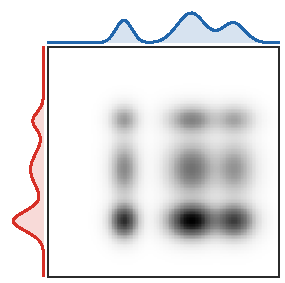
\includegraphics[width=.31\linewidth]{figures/kantorovich-coupling-matrix-marginals/product-200.pdf}\hspace{.045\linewidth}
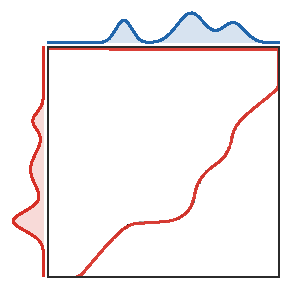
\includegraphics[width=.31\linewidth]{figures/kantorovich-coupling-matrix-marginals/optimal-200.pdf}
\caption{\emph{Couplings have the same marginals but different dependence.} The red and blue curves give the prescribed row and column masses. The independent coupling is diffuse, whereas the one-dimensional quadratic optimal plan follows the quantile correspondence. The matrix entries are transported masses, not conditional probabilities.}
\label{fig:kantorovich-coupling-matrix-marginals}
\end{figure}

\paragraph{Dual potentials.}
The dual variables are scalar functions whose sum stays below the cost. For continuous costs on compact spaces,
\begin{equation}\label{eq-primer-kantorovich-duality}
  \MK_c(\alpha,\beta)=
  \sup_{f(x)+g(y)\leq c(x,y)}
  \left\{\int f\,\d\alpha+\int g\,\d\beta\right\}.
\end{equation}
The supremum can be taken over continuous potentials. Integrating the constraint gives weak duality; equality is Kantorovich duality~\citep{Villani09}. When both optima exist, $f(x)+g(y)=c(x,y)$ for $\pi$-almost every transported pair. Potentials are unchanged as a certificate under $(f,g)\mapsto(f+a,g-a)$. Their dynamic counterparts will be Hamilton--Jacobi potentials.

\subsection{Wasserstein Geometry}
\label{sec-kantorovich-metric}

When cost is a power of a ground distance, the optimal value defines a geometry on laws. The quadratic Euclidean case is the metric underlying most PDEs in the review.

\paragraph{Distance, moments and convergence.}
Fix $1\leq p<+\infty$ and $x_0\in\X$. The finite-moment space and its transport distance are
\begin{defn}[Wasserstein space and distance]\label{def-wasserstein-distance}
\begin{align}
  \Pp_p(\X)&\eqdef\left\{\alpha\in\Pp(\X):\int d(x,x_0)^p\,\d\alpha(x)<+\infty\right\},
  \label{eq-primer-p-moment-space}\\
  \Wass_p(\alpha,\beta)&\eqdef
  \left(\inf_{\pi\in\Couplings(\alpha,\beta)}\int d(x,y)^p\,\d\pi(x,y)\right)^{1/p}.
  \label{eq-kantorovich-wasserstein}
\end{align}
\end{defn}
The moment condition is independent of $x_0$. The metric is finite on $\Pp_p(\X)$ and satisfies $\Wass_p(\delta_x,\delta_y)=d(x,y)$. This space is complete and separable whenever $\X$ is~\citep{Villani09,ambrosio2006gradient}.

The triangle inequality is a gluing argument that will recur below. Disintegrate couplings of $(\alpha,\beta)$ and $(\beta,\gamma)$ over their common marginal to obtain a triple $(X,Y,Z)$ with the two prescribed pair laws. Then $d(X,Z)\leq d(X,Y)+d(Y,Z)$ and Minkowski's inequality bound the cost of the induced $(X,Z)$ coupling. Optimizing proves the triangle inequality. For discrete plans, the glued matrix is $\P\operatorname{diag}(\b)^{-1}\Q$ after discarding zero-mass intermediate atoms.

Weak convergence, written $\alpha_n\rightharpoonup\alpha$, means convergence of integrals against all bounded continuous test functions. For $\alpha_n,\alpha\in\Pp_p(\X)$,
\begin{equation}\label{eq-primer-wasserstein-convergence}
  \Wass_p(\alpha_n,\alpha)\longrightarrow0
  \quad\Longleftrightarrow\quad
  \begin{cases}
    \alpha_n\rightharpoonup\alpha,\\
    \displaystyle\int d(x,x_0)^p\,\d\alpha_n(x)
    \longrightarrow\int d(x,x_0)^p\,\d\alpha(x).
  \end{cases}
\end{equation}
Thus weak convergence alone does not control mass escaping to infinity. Tightness together with uniform integrability of the $p$th moments gives relative Wasserstein compactness; a mere uniform $p$th-moment bound is not enough. On compact $\X$, no tail condition is needed.

\paragraph{Brenier maps.}
The central existence theorem converts a quadratic optimal coupling into a gradient map. This is the structural fact needed for displacement convexity and Gaussian transport.
\begin{thm}[Brenier]\label{thm-brenier}
If $\alpha,\beta\in\Pp_2(\RR^d)$ and $\alpha$ has a Lebesgue density, the unique quadratic optimal coupling is $(\Id,T)_\sharp\alpha$, where $T=\nabla\varphi$ for a convex potential $\varphi$, uniquely defined as a map $\alpha$-almost everywhere.
\end{thm}
The mechanism is that optimality prevents cost-reducing cyclic reassignments of transported pairs. Such pairs lie in the subdifferential of a convex function: $y\in\partial\varphi(x)$ means $\varphi(z)\geq\varphi(x)+\dotp{y}{z-x}$ for every $z$. This subdifferential is single-valued almost everywhere for an absolutely continuous source~\citep{Brenier91,Villani09}. If the map and both positive densities are smooth,~\eqref{eq-pfwd-density} becomes
\begin{equation}\label{eq-monge-ampere}
  \rho_\alpha(x)=\rho_\beta(\nabla\varphi(x))\det\nabla^2\varphi(x).
\end{equation}
This Monge--Amp\`ere identity is a change-of-variables equation; the weak transport theorem does not assume that its classical derivatives exist.

\paragraph{Displacement interpolation.}\label{sec-kantorovich-plan-interpolation}
A static optimal plan also specifies a time-dependent path by moving each paired particle along its joining segment.
\begin{defn}[Displacement interpolation]\label{def-w2-geodesic-induced-by-plan}
For $\alpha_0,\alpha_1\in\Pp_2(\RR^d)$ and a quadratic optimal coupling $\pi$, set
\begin{equation}\label{eq-plan-interpolation}
  \alpha_t=((1-t)P_0+tP_1)_\sharp\pi,
  \qquad P_0(x,y)=x,\quad P_1(x,y)=y,\quad 0\leq t\leq1.
\end{equation}
\end{defn}
It is a constant-speed geodesic: $\Wass_2(\alpha_s,\alpha_t)=|s-t|\Wass_2(\alpha_0,\alpha_1)$. Indeed, matching each endpoint pair to itself at times $s,t$ gives the upper bound, and the triangle inequality between the endpoints forces equality. In the map case, this reduces to McCann's interpolation $\alpha_t=((1-t)\Id+tT)_\sharp\alpha_0$. Moving every transported pair along a segment is the Lagrangian prototype of the Benamou--Brenier formulation in Section~\ref{sec-benamou-brenier-dynamic}.
On a general geodesic space, replace each segment by a metric geodesic and use a law of such paths; the same endpoint-coupling argument gives a Wasserstein geodesic whenever the required measurable choice exists.

\paragraph{Gaussian model.}\label{sec-gaussian-bures}
Gaussian laws provide the main exactly solvable example used later. For any $\alpha\in\Pp_2(\RR^d)$, its mean and covariance are $m_\alpha=\int x\,\d\alpha(x)$ and $\Sigma_\alpha=\int(x-m_\alpha)(x-m_\alpha)^\top\d\alpha(x)$; its raw second moment is $\Sigma_\alpha+m_\alpha m_\alpha^\top$. Write $\alpha=\Gaussian(m_\alpha,\Sigma_\alpha)$ and $\beta=\Gaussian(m_\beta,\Sigma_\beta)$ in the Gaussian case. In dimension one, covariance is variance $\sigma^2$, whereas $\sigma$ denotes standard deviation.
\begin{prop}[Gaussian quadratic transport]\label{prop-gaussian-w2-bures}
If $\Sigma_\alpha,\Sigma_\beta\succ0$, the Brenier map is
\begin{equation}\label{eq-bures-map}
  T(x)=m_\beta+A(x-m_\alpha),\qquad
  A=\Sigma_\alpha^{-1/2}(\Sigma_\alpha^{1/2}\Sigma_\beta\Sigma_\alpha^{1/2})^{1/2}\Sigma_\alpha^{-1/2}.
\end{equation}
Moreover,
\begin{equation}\label{eq-dist-gauss}
  \Wass_2^2(\alpha,\beta)=|m_\alpha-m_\beta|^2+\Bb^2(\Sigma_\alpha,\Sigma_\beta),\qquad
  \Bb^2(\Sigma,\Lambda)=\tr\bigl(\Sigma+\Lambda-2(\Sigma^{1/2}\Lambda\Sigma^{1/2})^{1/2}\bigr).
\end{equation}
The distance formula extends to positive semidefinite covariances by continuity.
\end{prop}
\begin{proof}
The displayed $A$ is symmetric positive definite and satisfies $A\Sigma_\alpha A=\Sigma_\beta$. Its affine map therefore has the correct Gaussian image and is a convex gradient, hence is optimal by Brenier's theorem. Taking the expected squared displacement gives the formula; approximation by positive definite covariances gives the final assertion.
\end{proof}
The covariance follows $\Sigma_t=((1-t)\Id+tA)\Sigma_\alpha((1-t)\Id+tA)$, not a linear interpolation of covariance entries. In dimension one, the squared distance is $(m_\alpha-m_\beta)^2+(\sigma_\alpha-\sigma_\beta)^2$ and both mean and standard deviation interpolate linearly. Gaussian preservation by a general flow is a separate question, addressed in Section~\ref{sec-gaussian-closure-transport-dynamics}.

The same geometry is particularly explicit on the line, where ordering supplies the optimal coupling.
\begin{example}[One-dimensional transport and quantiles]\label{ex-primer-quantile-transport}
For $\alpha\in\Pp(\RR)$, let $\cumul\alpha(x)=\alpha(( -\infty,x])$ and $\cumul\alpha^{-1}(r)=\inf\{x:\cumul\alpha(x)\geq r\}$ for $0<r<1$. The monotone coupling and its cost are
\begin{equation}\label{eq-primer-quantile-wasserstein}
  \pi=(\cumul\alpha^{-1},\cumul\beta^{-1})_\sharp\mathcal U_{(0,1)},
  \qquad
  \Wass_p^p(\alpha,\beta)=\int_0^1|\cumul\alpha^{-1}(r)-\cumul\beta^{-1}(r)|^p\,\d r.
\end{equation}
Here $\mathcal U_{(0,1)}$ is the uniform law on $(0,1)$. This coupling is optimal for every $1\leq p<+\infty$, including for atomic laws. Convexity of $|x-y|^p$ gives the uncrossing inequality, and approximation yields the general formula. If $\alpha$ is atomless, $T=\cumul\beta^{-1}\circ\cumul\alpha$ induces this coupling. For endpoints in $\Pp_2(\RR)$, a quadratic geodesic therefore has quantile $(1-t)\cumul{\alpha_0}^{-1}+t\cumul{\alpha_1}^{-1}$; Figure~\ref{fig:monge-1d-quantile-geodesic} illustrates this linearization.

\end{example}

\begin{figure}[htbp]
\centering
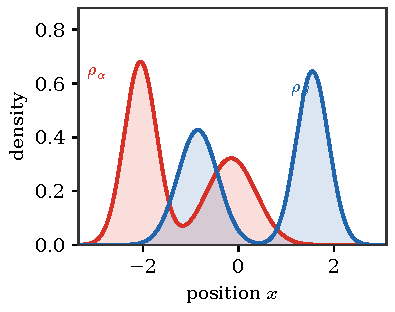
\includegraphics[width=.31\linewidth]{figures/monge-1d-quantile-geodesic/endpoint-densities.pdf}
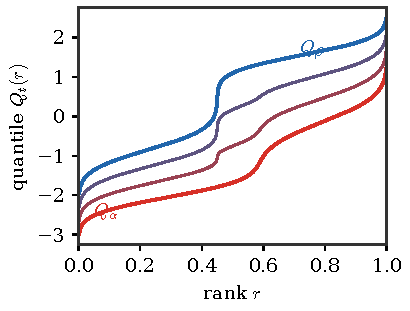
\includegraphics[width=.31\linewidth]{figures/monge-1d-quantile-geodesic/quantiles.pdf}
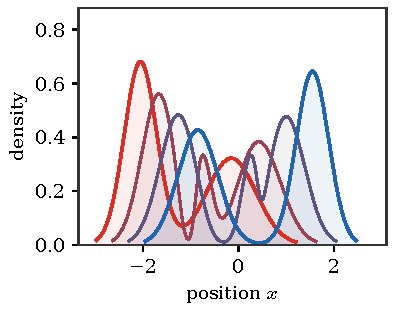
\includegraphics[width=.31\linewidth]{figures/monge-1d-quantile-geodesic/geodesic-densities.pdf}
\caption{\emph{One-dimensional displacement interpolation is linear in quantile coordinates.} Endpoint densities are shown on the left, inverse cumulative functions in the middle, and the induced density path on the right. The latter is generally not a linear mixture of the endpoint densities.}
\label{fig:monge-1d-quantile-geodesic}
\end{figure}

\subsection{Energies, Entropy and Kernel Discrepancies}
\label{sec-primer-functionals-discrepancies}

The metric specifies how a distribution moves, while a functional $f(\alpha)$ specifies what decreases. Linear potentials $\int V\,\d\alpha$, internal energies $\int U(\rho_\alpha)\,\d x$ and interactions $\frac12\iint W(x,y)\,\d\alpha(x)\d\alpha(y)$ will produce drift, diffusion and collective forces. We fix only the discrepancy conventions needed below; first variations are defined once, in Section~\ref{sec-wasserstein-gradient-flows}.

\paragraph{Divergences and density conventions.}
Density-ratio divergences include the entropy driving Fokker--Planck equations and the power family used in displacement-convexity examples. Their singular-mass convention is important for particle laws.
\begin{defn}[$\phi$-divergence and relative entropy]\label{def_divergence}\label{def-measure-relative-entropy}
Let $\phi:[0,+\infty)\to[0,+\infty]$ be convex and lower semicontinuous with $\phi(1)=0$. For probability measures, decompose $\alpha=r\beta+\alpha^\perp$, where $\alpha^\perp$ is singular with respect to $\beta$. Set
\begin{equation}\label{eq-phi-div}
  \Divergm_\phi(\alpha\mid\beta)
  \eqdef\int\phi(r)\,\d\beta+\phi'_\infty\alpha^\perp(\X),
  \qquad \phi'_\infty=\lim_{s\to+\infty}\phi(s)/s.
\end{equation}
We use $+\infty\cdot0=0$. Relative entropy $\KL(\alpha\mid\beta)$ corresponds to $\phi(r)=r\log r-r+1$, with $0\log0=0$. It is infinite if $\alpha\not\ll\beta$.
\end{defn}
When $\alpha\ll\beta$, this simplifies to
\begin{equation}\label{eq-primer-relative-entropy}
  \KL(\alpha\mid\beta)=\int\log(\d\alpha/\d\beta)\,\d\alpha.
\end{equation}
Shannon neg-entropy is instead $\mathcal H(\alpha)=\int\rho_\alpha\log\rho_\alpha\,\d x$, with value $+\infty$ for singular laws and with the usual finite-value or extended-integral qualifications. Lebesgue measure on $\RR^d$ is not a probability reference, so this expression should not be confused with~\eqref{eq-primer-relative-entropy}. If $\beta=Z^{-1}e^{-V}\d x$, relative entropy differs from $\mathcal H(\alpha)+\int V\,\d\alpha$ only by the constant $\log Z$.

\paragraph{Kernel energies.}\label{sec-rkhs-mmd}
Kernel discrepancies produce the interaction fields used in particle sampling. The following convention also permits the distance kernels appearing in the one-dimensional convexity examples.
\begin{defn}[Kernel discrepancy]\label{def-kernel-mmd-norm}\label{def-positive-kernels}
A symmetric kernel $k$ is positive semidefinite if $\sum_{i,j}u_i u_jk(x_i,x_j)\geq0$ for every finite family; it is conditionally positive semidefinite if this is required only when $\sum_i u_i=0$. For probability laws with absolutely integrable kernel energy, define
\begin{equation}\label{eq-primer-mmd}
  \MMD_k^2(\alpha,\beta)\eqdef
  \iint k(x,y)\,\d(\alpha-\beta)(x)\d(\alpha-\beta)(y).
\end{equation}
\end{defn}
For a positive semidefinite kernel, its reproducing-kernel Hilbert space (RKHS) $\RKHS_k$ satisfies $h(x)=\langle h,k(x,\cdot)\rangle_{\RKHS_k}$. The discrepancy is the squared norm of $\int k(x,\cdot)\,\d(\alpha-\beta)(x)$ whenever that Bochner integral exists. For a conditionally positive kernel, anchor at a point $o$: $k^o(x,y)=k(x,y)-k(x,o)-k(o,y)+k(o,o)$ is positive semidefinite and gives the same zero-mass energy. This covers $k(x,y)=-|x-y|$ on the line. Gaussian and Laplace kernels give familiar bounded examples; $k(x,y)=\dotp xy^2$ compares raw second moments. Nonnegativity does not imply separation for every kernel. A kernel is called characteristic when $\MMD_k(\alpha,\beta)=0$ forces $\alpha=\beta$ on the class of laws under consideration. The interaction velocities associated with~\eqref{eq-primer-mmd} are derived in Section~\ref{sec-wasserstein-gradient-flows}.


\FloatBarrier

% !TEX root = ../PDE4ML.tex

\section{Dynamic Optimal Transport}
\index{dynamic!optimal transport}% strictindex
\label{sec-dynamic-optimal-transport}

Optimal transport becomes especially powerful once distances between measures are seen as actions of moving mass. Continuity equations connect particle trajectories to evolving distributions, and the Benamou--Brenier formula identifies quadratic Wasserstein distance with a least-action principle. We develop its velocity, momentum and Hamilton--Jacobi descriptions, together with the equivalent path-space viewpoint. These are the tools needed for gradient flows and generative dynamics in the following sections.
\index{continuity equation}% strictindex
\index{generative model}% strictindex
\index{Benamou-Brenier@Benamou--Brenier}% strictindex
\index{gradient!flow}% strictindex
\index{Benamou-Brenier@Benamou--Brenier!formula}% strictindex

\subsection{Evolutions over the Space of Measures}
\index{measure!evolution}% strictindex

We start with the continuity equation because it is the common language for particles, densities and weak measure evolutions. It also makes precise which velocity fields actually move mass.
\index{velocity field}% strictindex
\index{continuity equation}% strictindex

\paragraph{Lagrangian and Eulerian descriptions.}
\index{Lagrangian!description}% strictindex
\index{Eulerian!description}% strictindex

We consider the evolution $t \mapsto \alpha_t \in \Pp(\RR^d)$. Such an evolution can be described in a Lagrangian way as the advection of particles along a (time-dependent) vector field $v_t(x)$ in $\RR^d$. At the particle level, this advection is governed by
\index{time-dependent vector field}% strictindex
\begin{equation}
    \frac{\d x(t)}{\d t} = v_t(x(t)), \label{eq:lagrangian-advection}
\end{equation}
When the ODE is well posed, for instance for a spatially Lipschitz velocity of at most linear growth with time-integrable bounds, we write $T_t$ for its flow map, so that $T_t(x(0))=x(t)$. The advected measure is then $\alpha_t = (T_t)_\sharp \alpha_0$. For discrete measures, $\alpha_t = \frac{1}{n} \sum_{i=1}^n \delta_{x_i(t)}$, meaning each $x_i(t)$ solves \eqref{eq:lagrangian-advection}.
\index{flow!map}% strictindex

In the Eulerian description, the same motion is written directly on the evolving measure: the particle ODE becomes the PDE
\index{particle ODE}% strictindex
\index{Eulerian!description}% strictindex
\begin{equation}
    \frac{\partial \alpha_t}{\partial t} + \diverg(v_t \alpha_t) = 0. \label{eq:eulerian-advection}
\end{equation}
This PDE is often referred to as the advection equation, the continuity equation, or Liouville's equation when operating over a phase space. It is only a classical PDE when $\alpha_t$ has a smooth density. For general measures, and in particular for empirical measures, it is understood in the distributional sense: for every $\varphi\in C_c^1((0,1)\times\RR^d)$,
\index{empirical!measure}% strictindex
\index{continuity equation}% strictindex
\begin{equation}\label{eq:eulerian-advection-weak}
	\int_0^1\!\int_{\RR^d}
	\left(\partial_t\varphi(t,x)+\dotp{v_t(x)}{\nabla_x\varphi(t,x)}\right)
	\d\alpha_t(x)\d t
	=
	0.
\end{equation}
This equation is obtained from~\eqref{eq:eulerian-advection} by integration by parts. Hence, for smooth positive densities, the classical and weak formulations are equivalent; the weak formulation is useful because it still makes sense for discrete measures whose particles evolve according to~\eqref{eq:lagrangian-advection}.

This interior identity provides the measure-theoretic notion of an admissible evolution. To include endpoint traces and, on a bounded domain, an impermeable boundary in the same formula, one tests up to the temporal and spatial boundaries.
\begin{defn}[Admissible continuity-equation evolution]\label{def-admissible-continuity-evolution}
\index{continuity equation!admissible evolution}% strictindex
Let $\Omega=\RR^d$, or let $\Omega\subset\RR^d$ be a bounded Lipschitz domain. A narrowly (weakly) continuous curve $(\alpha_t)_{t\in[0,1]}$ in $\Pp(\overline\Omega)$ and a jointly Borel velocity field $v:(t,x)\mapsto v_t(x)$ are admissible between $\alpha_0$ and $\alpha_1$ if
\[
\int_0^1\!\int_{\overline\Omega}\norm{v_t(x)}^2\d\alpha_t(x)\d t<+\infty
\]
and, for every $\varphi\in C^1([0,1]\times\overline\Omega)$, with compact spatial support when $\Omega=\RR^d$,
\begin{equation}\label{eq-continuity-endpoint-no-flux}
\int_0^1\!\int_{\overline\Omega}
\left(\partial_t\varphi+\dotp{v_t}{\nabla_x\varphi}\right)\d\alpha_t\d t
+\int_{\overline\Omega}\varphi(0,\cdot)\d\alpha_0
-\int_{\overline\Omega}\varphi(1,\cdot)\d\alpha_1=0.
\end{equation}
On a bounded domain, allowing test functions that do not vanish on $\partial\Omega$ encodes the zero-normal-flux condition $(\alpha_t v_t)\cdot n=0$ weakly.
\end{defn}

\begin{prop}[Lagrangian flows solve the continuity equation]\label{prop-lagrangian-flow-continuity}
\index{Lagrangian!flow}% strictindex
\index{continuity equation}% strictindex
	Let $(T_t)_{t\in[0,1]}$ be a $C^1$ family of diffeomorphisms of $\RR^d$, with $T_0=\Id$, and define $\alpha_t=(T_t)_\sharp\alpha_0$. Assume that the derivatives below are integrable with respect to $\alpha_0$, and define the Eulerian velocity field by
\index{velocity field}% strictindex
\index{Eulerian!velocity}% strictindex
	\[
		v_t(T_t(y))=\partial_t T_t(y).
	\]
	Then $(\alpha_t,v_t)$ solves the continuity equation in the weak sense~\eqref{eq:eulerian-advection-weak}.
	In particular, if $\alpha_0=\frac1n\sum_i\delta_{x_i(0)}$ is empirical, then $\alpha_t=\frac1n\sum_i\delta_{x_i(t)}$ is empirical as well, with particle velocities $\dot x_i(t)=v_t(x_i(t))$.
\end{prop}

\begin{proof}
	Let $\varphi\in C_c^1((0,1)\times\RR^d)$. Since $\alpha_t=(T_t)_\sharp\alpha_0$,
	\[
		\frac{\d}{\d t}\int \varphi(t,x)\d\alpha_t(x)
		=
		\frac{\d}{\d t}\int \varphi(t,T_t(y))\d\alpha_0(y).
	\]
	The chain rule gives
	\[
		\frac{\d}{\d t}\int \varphi(t,T_t(y))\d\alpha_0(y)
		=
		\int
		\left(
			\partial_t\varphi(t,T_t(y))
			+\dotp{\nabla_x\varphi(t,T_t(y))}{\partial_t T_t(y)}
		\right)
		\d\alpha_0(y).
	\]
	Using the definition of $v_t$ and the push-forward relation, this equals
\index{push-forward}% strictindex
	\[
		\int
		\left(
			\partial_t\varphi(t,x)+\dotp{\nabla_x\varphi(t,x)}{v_t(x)}
		\right)
		\d\alpha_t(x).
	\]
	Integrating in time and using the boundary values of $\varphi$ gives~\eqref{eq:eulerian-advection-weak}.
\end{proof}

\paragraph{From measure evolutions to vector fields.}
\index{measure!evolution}% strictindex

For a given evolution $(\alpha_t)_t$, there are typically infinitely many velocity fields $v_t$ satisfying
\index{velocity field}% strictindex
\begin{equation}\label{eq:inverse-flow}
	\partial_t\alpha_t+\diverg(\alpha_t v_t)=0.
\end{equation}
This non-uniqueness comes from the kernel of the weighted divergence. The linear space of vector fields that leave a measure $\alpha$ invariant is
\[
	\Hh_\alpha=\enscond{v\in L^2(\alpha;\RR^d)}{\diverg(\alpha v)=0\ \text{in distributions}}.
\]
It is usually non-trivial: for instance, if $\alpha$ is an isotropic Gaussian, $\Hh_\alpha$ contains rotational vector fields generated by anti-symmetric matrices.

The orthogonal complement of this kernel is the Wasserstein tangent space
\begin{equation}\label{eq-wasserstein-tangent-space}
\operatorname{Tan}_\alpha\Pp_2
\eqdef\overline{\{\nabla\psi:\psi\in C_c^\infty(\RR^d)\}}^{L^2(\alpha)}
=\Hh_\alpha^\perp.
\end{equation}
Indeed, the distributional condition defining $\Hh_\alpha$ is precisely orthogonality to all test gradients. Projecting any finite-energy admissible velocity onto this tangent space leaves its continuity equation unchanged and gives the unique minimum-norm representative. This is the gradient representative used throughout the review~\citep{ambrosio2006gradient}.

\paragraph{Dacorogna--Moser inversion.}
\index{Dacorogna-Moser@Dacorogna--Moser!inversion}% strictindex
\index{Dacorogna-Moser@Dacorogna--Moser!construction}% strictindex

Reconstructing particles from an observed density evolution is therefore ill-posed. For a smooth positive density $\alpha_t=\rho_t\,\d x$, a simple choice, introduced by Dacorogna and Moser~\citep{DacorognaMoser1990}, is to impose that the flux $\rho_t v_t$ is a gradient field. With a fixed convention for the inverse Laplacian, this gives formally
\index{flux}% strictindex
\begin{equation}\label{eq:dacorogna-moser}
	v_t=-\frac{1}{\rho_t}\nabla\Delta^{-1}(\partial_t\rho_t),
\end{equation}
with suitable boundary conditions, for instance vanishing at infinity. This formula is useful conceptually but delicate when $\rho_t$ vanishes, and it does not generally produce a gradient velocity field.
\index{velocity field}% strictindex
\index{gradient!velocity}% strictindex

The classical Dacorogna--Moser construction uses the linear density path. If $\alpha_i=\rho_i\,\d x$ are smooth densities, bounded away from zero on the closure of a bounded connected domain $\Omega$ with smooth boundary, and have the same total mass, set
\[
	\alpha_t=(1-t)\alpha_0+t\alpha_1=\rho_t\,\d x,
	\qquad
	\rho_t=(1-t)\rho_0+t\rho_1.
\]
Choose a time-independent flux $w$ satisfying
\[
	\diverg w=\rho_0-\rho_1,
	\qquad
	w\cdot n=0\quad\hbox{on }\partial\Omega,
\]
for instance $w=-\nabla\phi$ with $\Delta\phi=\rho_1-\rho_0$ and Neumann boundary condition. Then
\[
	v_t=\frac{w}{\rho_t}
\]
satisfies $\partial_t\rho_t+\diverg(\rho_t v_t)=0$. The flow
$\partial_t T_t=v_t\circ T_t$, $T_0=\Id$, therefore transports
$\rho_0\d x$ onto $\rho_t\d x$, and $T_1$ solves the prescribed-Jacobian problem
$\rho_1(T_1(x))\det(\nabla T_1(x))=\rho_0(x)$.

\paragraph{Least-square inversion and gradient structure.}
\index{least squares!inversion}% strictindex
\index{gradient!structure}% strictindex

A more geometric choice, underlying optimal transport and Wasserstein gradient flows, is to select among all admissible velocities the one with smallest kinetic energy:
\index{Wasserstein!gradient}% strictindex
\index{gradient!flow}% strictindex
\index{Wasserstein!gradient flow}% strictindex
\index{flow matching}% strictindex
\begin{equation}\label{eq:least-square-field}
	\umin{v}
	\frac12\int_0^1\!\int_{\RR^d}\norm{v_t(x)}^2\,\d\alpha_t(x)\d t
	\quad
	\text{subject to}
	\quad
	\partial_t\alpha_t+\diverg(\alpha_t v_t)=0.
\end{equation}

\begin{prop}[Least-square velocities are gradients]\label{prop-least-square-gradient-velocity}
\index{least squares!velocity}% strictindex
\index{gradient!velocity}% strictindex
	Assume that $\alpha_t=\rho_t\,\d x$ is a smooth positive density curve, that $\partial_t\rho_t$ has zero integral, and that boundary terms vanish. The minimizer of~\eqref{eq:least-square-field}, if it exists, is a gradient field
	\[
		v_t=\nabla\phi_t,
	\]
	where $\phi_t$, unique up to an additive constant on each connected component, solves the weighted Poisson equation
\index{weighted!Poisson equation}% strictindex
	\begin{equation}\label{eq:least-square-field-explicit}
		-\diverg(\rho_t\nabla\phi_t)=\partial_t\rho_t,
		\qquad
		v_t=-\nabla\Delta_{\alpha_t}^{-1}(\partial_t\alpha_t),
		\quad
		\Delta_{\alpha_t}\phi=\diverg(\alpha_t\nabla\phi).
	\end{equation}
\end{prop}

\begin{proof}
	Introduce a Lagrange multiplier $\phi_t$ for the continuity equation. The constrained problem has the formal saddle formulation
\index{continuity equation}% strictindex
	\[
		\umin{v}\umax{\phi}
		\int_0^1
		\left[
			\frac12\int_{\RR^d}\norm{v_t(x)}^2\,\d\alpha_t(x)
			+\int_{\RR^d}\phi_t(x)\big(\diverg(\rho_t v_t)(x)+\partial_t\rho_t(x)\big)\d x
		\right]\d t.
	\]
	Integrating by parts in the divergence term gives, for each $t$,
	\[
		\int \left(\frac12\norm{v_t}^2-\dotp{\nabla\phi_t}{v_t}\right)\d\alpha_t
		+
		\int \phi_t\,\partial_t\rho_t\,\d x.
	\]
	The pointwise minimizer in $v_t$ is therefore $v_t=\nabla\phi_t$. Substituting this into the constraint $\partial_t\rho_t+\diverg(\rho_t v_t)=0$ gives the weighted Poisson equation in~\eqref{eq:least-square-field-explicit}. The inverse notation is just a shorthand for solving this equation on zero-mean right-hand sides, modulo additive constants.
\index{zero mean}% strictindex
\index{weighted!Poisson equation}% strictindex
\end{proof}

This minimum-energy inversion can be computationally demanding. Flow matching in Section~\ref{sec-generative-flow-matching} instead constructs an admissible velocity by conditional regression; it need not be the minimum-energy representative of the same density evolution.
\index{flow matching}% strictindex

\subsection{Benamou--Brenier Dynamic Formulation of OT}
\index{Benamou-Brenier@Benamou--Brenier}% strictindex
\index{Benamou-Brenier@Benamou--Brenier!formulation}% strictindex
\index{Benamou-Brenier@Benamou--Brenier!formula}% strictindex
\label{sec-benamou-brenier-dynamic}

The dynamic formulation identifies $\Wass_2$ with the kinetic energy of the cheapest continuity-equation path. It is the point where OT becomes a least-action principle.
\index{continuity equation}% strictindex
\index{dynamic!formulation}% strictindex

\paragraph{Benamou--Brenier formulation.}

Instead of assuming that a whole curve $(\alpha_t)_{t\in[0,1]}$ is prescribed, one only fixes its endpoints $\alpha_0$ and $\alpha_1$ and minimizes the least-square energy~\eqref{eq:least-square-field}. The theorem of Benamou and Brenier states that twice this least-square energy, or equivalently the unhalved action defined below, is exactly the squared Wasserstein distance~\citep{benamou2000computational}.
\index{Wasserstein!distance}% strictindex

The kinetic energy of an admissible evolution is the basic dynamic action.
\begin{defn}[Benamou--Brenier action]\label{def-benamou-brenier-action}
For an admissible pair $(\alpha_t,v_t)$, define
\[
\operatorname{Act}_2(\alpha,v)
\eqdef
\int_0^1\!\int_{\RR^d}\norm{v_t(x)}^2\d\alpha_t(x)\d t.
\]
\end{defn}

\begin{thm}[Benamou--Brenier]\label{thm-benamou-brenier}
\index{Benamou-Brenier@Benamou--Brenier}% strictindex
	For probability measures $\alpha_0,\alpha_1\in\Pp_2(\RR^d)$,
\index{probability measure}% strictindex
	\begin{equation}\label{eq:benamou-brenier}
	\Wass_2^2(\alpha_0,\alpha_1)
	=
	\inf_{(\alpha_t,v_t)}
	\int_0^1\!\int_{\RR^d}\norm{v_t(x)}^2\,\d\alpha_t(x)\d t,
	\end{equation}
	where the infimum is over admissible pairs in Definition~\ref{def-admissible-continuity-evolution}, with $\alpha_t\in\Pp_2(\RR^d)$, solving $\partial_t\alpha_t+\nabla\!\cdot(\alpha_t v_t)=0$ with $\alpha_{t=0}=\alpha_0$ and $\alpha_{t=1}=\alpha_1$. If $\alpha_0$ has a density and $T$ is the optimal Monge map $T_\sharp\alpha_0=\alpha_1$, a minimizing curve is
\index{Monge!problem}% strictindex
	\begin{equation}\label{eq:static-to-dynamic}
		\alpha_t=((1-t)\Id+tT)_\sharp\alpha_0,
		\qquad
		v_t\big((1-t)x+tT(x)\big)=T(x)-x
		\quad\text{for $\alpha_0$-a.e.\ $x$ and a.e.\ $t\in(0,1)$}.
	\end{equation}
\end{thm}

\begin{proof}
	For the inequality ``dynamic $\leq$ static'', assume first that a Monge map $T$ exists and define $(\alpha_t,v_t)$ by~\eqref{eq:static-to-dynamic}. Since the Lagrangian velocity $T(x)-x$ is independent of $t$,
\index{Monge!problem}% strictindex
	\[
		\int_0^1\!\int\norm{v_t}^2\,\d\alpha_t\d t
		=
		\int\norm{T(x)-x}^2\,\d\alpha_0(x),
	\]
	so the dynamic cost is no larger than the static Monge cost. Without a Monge map, the same construction is made with an optimal coupling $\pi$: sample $(X,Y)\sim\pi$ and move along the straight path $\gamma_{X,Y}(t)=(1-t)X+tY$. This path measure has action $\int\norm{x-y}^2\d\pi(x,y)$; projecting path velocities onto their conditional mean at time $t$ gives an admissible Eulerian velocity with no larger action, so the dynamic value is no larger than the Kantorovich value.
\index{dynamic!value}% strictindex
\index{optimal coupling}% strictindex
\index{Eulerian!velocity}% strictindex
\index{path measure}% strictindex

	Conversely, for a smooth deterministic path, take the flow $T_t$ defined by $\dot T_t=v_t\circ T_t$ and $T_0=\Id$. Then $\alpha_t=(T_t)_\sharp\alpha_0$ and $(T_1)_\sharp\alpha_0=\alpha_1$. Jensen's inequality gives
\index{Jensen inequality}% strictindex
	\[
		\norm{T_1(x)-x}^2
		\leq
		\int_0^1\norm{v_t(T_t(x))}^2\d t.
	\]
	After integration with respect to $\alpha_0$, the Monge cost is bounded above by the dynamic action. For general finite-energy solutions of the continuity equation, the superposition principle~\citep{ambrosio2006gradient} lifts the curve to a probability measure on absolutely continuous paths; applying Jensen's inequality pathwise gives a coupling of the endpoints whose quadratic cost is no larger than the action. Thus the Kantorovich value is bounded above by the dynamic value.
\index{dynamic!value}% strictindex
\index{absolutely continuous path}% strictindex
\index{dynamic!action}% strictindex
\index{superposition principle}% strictindex
\index{Jensen inequality}% strictindex
\index{probability measure}% strictindex
\index{continuity equation}% strictindex
\index{quadratic!cost}% strictindex
\end{proof}

\paragraph{Convex momentum-based reformulation.}
\index{momentum formulation}% strictindex

Although~\eqref{eq:benamou-brenier} is not jointly convex in $(\alpha_t,v_t)$, it becomes convex after replacing velocities by momenta. Given a velocity \(v\in L^2(\alpha;\RR^d)\), define the momentum
\[
	\omega\eqdef \alpha v,
	\qquad
	\omega(A)=\int_A v(x)\,\d\alpha(x),
\]
which is a finite \(\RR^d\)-valued measure. Its total-variation measure is defined by $|\omega|(A)=\sup\sum_j\norm{\omega(A_j)}$, where the supremum runs over finite measurable partitions of $A$; its total mass is the vector-measure total-variation norm. If $\omega=v\alpha$, then $|\omega|=\norm v\alpha$. A reference $\lambda$ dominating $\alpha$ and $|\omega|$ therefore admits the scalar and vector Radon--Nikodym densities used below. The nonlinear relation \(\omega=\alpha v\) is eliminated by the following measure perspective.
\begin{defn}[Quadratic perspective action]\label{def-quadratic-perspective-action}
\begin{equation}\label{eq-quadratic-perspective}
	J(a,m)
	\eqdef
	\begin{cases}
		\norm{m}^2/a, & a>0,\\
		0, & a=0\ \text{and}\ m=0,\\
	+\infty, & a=0\ \text{and}\ m\neq0,
	\end{cases}
	\qquad
	(a,m)\in[0,+\infty)\times\RR^d.
\end{equation}
\index{perspective function}% strictindex
\index{quadratic!perspective}% strictindex
If \(\lambda\) dominates \(\alpha\) and \(|\omega|\), define
\begin{equation}\label{eq-measure-perspective-action}
	\mathbb J(\alpha,\omega)
	\eqdef
	\int
	J\left(
		\frac{\d\alpha}{\d\lambda}(x),
		\frac{\d \omega}{\d\lambda}(x)
	\right)\d\lambda(x).
\end{equation}
\end{defn}
\index{perspective function}% strictindex
\index{quadratic!perspective}% strictindex
The pointwise function is lower-semicontinuous, convex and positively \(1\)-homogeneous: \(J(\eta a,\eta m)=\eta J(a,m)\) for \(\eta>0\), with \(J(0,0)=0\).
The definition is independent of the dominating measure \(\lambda\): after replacing \(\lambda\) by another dominating measure, both Radon--Nikodym densities are rescaled by the same factor, which cancels with the change of reference measure by the \(1\)-homogeneity of \(J\). Equivalently, this is the standard integral functional associated with a convex normal integrand, used in the measure-valued relaxation of dynamic OT~\citep{ambrosio2006gradient}; see also Rockafellar's perspective construction~\citep{rockafellar2015convex}. In particular,
\[
	\mathbb J(\alpha,\omega)<+\infty
	\quad\Longleftrightarrow\quad
	\omega=v\alpha\ \text{with}\ v\in L^2(\alpha;\RR^d),
	\qquad
	\mathbb J(\alpha,\omega)=\int\norm{v}^2\,\d\alpha.
\]

The Benamou--Brenier problem can now be written with the linear continuity equation in the pair \((\alpha_t,\omega_t)\):
\index{perspective function}% strictindex
\index{momentum}% strictindex
\index{Benamou-Brenier@Benamou--Brenier}% strictindex
\begin{equation}\label{eq:benamou-brenier-convex}
	\Wass_2^2(\alpha_0,\alpha_1)
	=
	\inf_{\substack{\partial_t\alpha_t+\diverg \omega_t=0\\
	\alpha_{t=0}=\alpha_0,\ \alpha_{t=1}=\alpha_1}}
	\int_0^1 \mathbb J(\alpha_t,\omega_t)\,\d t.
\end{equation}
In the absolutely continuous case \(\alpha_t=\rho_t\,\d x\) and \(\omega_t=m_t\,\d x\), this becomes
\[
	\inf_{\substack{\partial_t\rho_t+\diverg m_t=0\\
	\rho_{t=0}\d x=\alpha_0,\ \rho_{t=1}\d x=\alpha_1}}
	\int_0^1\!\int_{\RR^d}
	J(\rho_t(x),m_t(x))\,\d x\,\d t
	=
	\inf_{\substack{\partial_t\rho_t+\diverg m_t=0\\
	\rho_{t=0}\d x=\alpha_0,\ \rho_{t=1}\d x=\alpha_1}}
	\int_0^1\!\int_{\RR^d}
	\frac{\norm{m_t(x)}^2}{\rho_t(x)}\,\d x\,\d t,
\]
with the conventions encoded in~\eqref{eq-quadratic-perspective}. This convex reformulation enables geodesic interpolation by convex optimization once the domain is discretized.
\index{recession convention}% strictindex
\index{momentum}% strictindex

\paragraph{Dual Hamilton--Jacobi formulation.}
\index{Hamilton-Jacobi@Hamilton--Jacobi equation}% strictindex
\index{Benamou-Brenier@Benamou--Brenier!dual}% strictindex

The momentum formulation also has a useful dual. It turns the least-action problem into a Hamilton--Jacobi subsolution inequality for a scalar potential, with equality on the part of space-time actually visited by the optimal curve. This is the dual dynamic formulation already present in the original Benamou--Brenier perspective~\citep{benamou2000computational}; see also the standard accounts~\citep{Villani03,SantambrogioBook}. The constants below follow the convention of~\eqref{eq:benamou-brenier-convex}, where the kinetic energy has no factor $1/2$.
\index{perspective function}% strictindex

\begin{prop}[Dual Benamou--Brenier problem]\label{prop-benamou-brenier-dual}
	Assume, for simplicity, that the densities are smooth, compactly supported, and that boundary terms vanish. Then the convex dynamic value~\eqref{eq:benamou-brenier-convex} has the dual formulation
	\begin{equation}\label{eq:benamou-brenier-dual}
		\Wass_2^2(\alpha_0,\alpha_1)
		=
		\sup_{\phi}
		\enscond{
		\int_{\RR^d}\phi_1\,\d\alpha_1
		-
		\int_{\RR^d}\phi_0\,\d\alpha_0
		}{
		\partial_t\phi_t+\frac14\norm{\nabla\phi_t}^2\leq 0
		},
	\end{equation}
	where the supremum is over smooth test potentials $\phi:[0,1]\times\RR^d\to\RR$. For nonsmooth Euclidean data, the same formula is understood in the relaxed formulation: $\phi$ is a Hamilton--Jacobi subsolution, for instance in the viscosity sense, and finite-dimensional discretizations follow directly from Fenchel--Rockafellar duality.
\index{Hamilton-Jacobi@Hamilton--Jacobi equation}% strictindex

	If $(\rho,m)$ and $\phi$ are smooth primal and dual optimizers, then
	\begin{equation}\label{eq:bb-primal-dual-relation}
		m_t=\frac{\rho_t}{2}\nabla\phi_t,
		\qquad
		\partial_t\phi_t+\frac14\norm{\nabla\phi_t}^2=0
		\quad\text{on }\{\rho_t>0\}.
	\end{equation}
	Equivalently, the optimal Eulerian velocity is $v_t=m_t/\rho_t=\nabla\phi_t/2$.
\index{Eulerian!velocity}% strictindex
\end{prop}

\begin{proof}
	Let $(\rho,m)$ satisfy the continuity equation and let $\phi$ be smooth. Multiplying the constraint by $\phi$ and integrating by parts gives
\index{continuity equation}% strictindex
	\[
		\int_{\RR^d}\phi_1\,\d\alpha_1
		-
		\int_{\RR^d}\phi_0\,\d\alpha_0
		=
		\int_0^1\!\int_{\RR^d}
		\left(\rho_t\,\partial_t\phi_t+\dotp{m_t}{\nabla\phi_t}\right)\d x\d t.
	\]
	If $\partial_t\phi_t+\norm{\nabla\phi_t}^2/4\leq0$, Young's inequality yields, pointwise,
	\[
		\rho\,\partial_t\phi+\dotp{m}{\nabla\phi}
		\leq
		-\frac{\rho}{4}\norm{\nabla\phi}^2+\dotp{m}{\nabla\phi}
		\leq
		J(\rho,m),
	\]
	with the perspective convention~\eqref{eq-quadratic-perspective}. Hence the dual objective of every feasible $\phi$ is no larger than the action of every feasible primal pair.
\index{perspective function}% strictindex

	Conversely, introduce $\phi$ as a Lagrange multiplier for $\partial_t\rho+\diverg m=0$. After integration by parts, and up to the fixed endpoint contribution in~\eqref{eq:benamou-brenier-dual}, the pointwise minimization over $(\rho,m)$ contains
	\[
		J(\rho,m)-\rho\,\partial_t\phi-\dotp{m}{\nabla\phi}.
	\]
	For fixed $\rho>0$, its minimum over $m$ is attained at $m=\rho\nabla\phi/2$ and equals $-\rho(\partial_t\phi+\norm{\nabla\phi}^2/4)$. The recession cases in~\eqref{eq-quadratic-perspective} give the same conclusion when \(\rho=0\). Thus the infimum over $\rho\geq0$ is finite exactly when the Hamilton--Jacobi inequality holds, in which case the pointwise infimum is $0$.

	This calculation identifies the dual but does not alone prove absence of a gap. One can justify equality from static Kantorovich duality~\eqref{eq-primer-kantorovich-duality}: the Hopf--Lax extension $\phi_t(y)=\inf_x\{\phi_0(x)+\norm{x-y}^2/t\}$ solves the Hamilton--Jacobi equation in the viscosity sense and realizes the quadratic static dual constraint at $t=1$. For compactly supported endpoints, approximation by smooth subsolutions preserves the supremum; see~\citet{Villani03,SantambrogioBook}. Finally, equality in the two pointwise inequalities gives~\eqref{eq:bb-primal-dual-relation}.
\index{Hamilton-Jacobi@Hamilton--Jacobi equation}% strictindex
\index{duality!Fenchel-Rockafellar@Fenchel--Rockafellar}% strictindex
\index{perspective function}% strictindex
\end{proof}

This also recovers the static Kantorovich inequality from a dynamic principle. If $\gamma$ is any smooth curve with $\gamma(0)=x$ and $\gamma(1)=y$, then
\[
	\frac{\d}{\d t}\phi_t(\gamma(t))
	=
	\partial_t\phi_t(\gamma(t))+\dotp{\nabla\phi_t(\gamma(t))}{\dot\gamma(t)}
	\leq
	\norm{\dot\gamma(t)}^2,
\]
where the last inequality uses $\partial_t\phi+\norm{\nabla\phi}^2/4\leq0$ and Young's inequality. Integrating and minimizing over curves gives
\[
	\phi_1(y)-\phi_0(x)\leq\norm{x-y}^2.
\]
Thus $(-\phi_0,\phi_1)$ is a feasible static Kantorovich dual pair for the quadratic cost. At optimality the inequality is saturated on the endpoint pairs connected by the primal characteristics, which is the Eulerian version of complementary slackness.
\index{Kantorovich!dual}% strictindex
\index{complementary slackness}% strictindex

Figure~\ref{fig:dynamic-benamou-brenier-duality} displays these primal--dual relations for a one-dimensional mixture transport, including the Hamilton--Jacobi contact identity along the active mass.

\begin{figure}[ht]
\centering
\begin{tabular}{@{}ccc@{}}
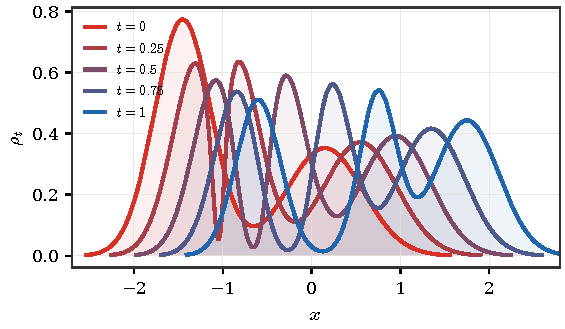
\includegraphics[width=.31\linewidth]{figures/dynamic-benamou-brenier-duality/density.pdf} &
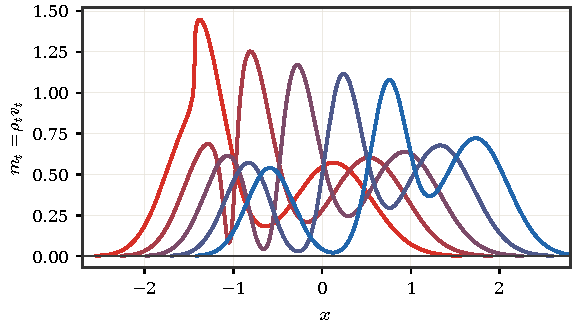
\includegraphics[width=.31\linewidth]{figures/dynamic-benamou-brenier-duality/momentum.pdf} &
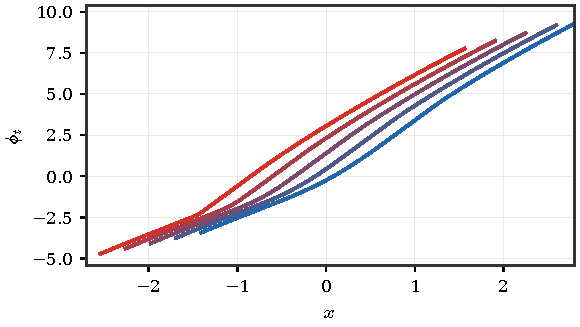
\includegraphics[width=.31\linewidth]{figures/dynamic-benamou-brenier-duality/dual-potential.pdf}
\\[-.1em]
\small density $\rho_t$ &
\small momentum density $m_t$ &
\small dual potential $\phi_t$
\end{tabular}
\caption{\emph{One-dimensional Benamou--Brenier primal and dual solutions.} The endpoints are Gaussian mixtures and the solution is computed from monotone quantile interpolation. The left and middle panels show the primal density and the momentum density $m_t=\rho_t v_t$. The right panel shows the dual Hamilton--Jacobi potential, normalized up to an additive constant. Along the active transported mass, the notebook checks the primal--dual identities $m_t=\rho_t\partial_x\phi_t/2$ and $\partial_t\phi_t+|\partial_x\phi_t|^2/4=0$.}
\index{Hamilton-Jacobi@Hamilton--Jacobi equation}% strictindex
\index{momentum}% strictindex
\label{fig:dynamic-benamou-brenier-duality}
\end{figure}

Figure~\ref{fig:dynamic-benamou-brenier-geodesic} complements the Eulerian optimization viewpoint with the Lagrangian picture: matched particles travel along the straight characteristics of the minimizing curve.

\begin{figure}[ht]
\centering
\newcommand{\bbgeodesicpanelheight}{.155\linewidth}
\begin{tabular}{@{}cc@{}}

\includegraphics[height=\bbgeodesicpanelheight]{figures/dynamic-benamou-brenier-geodesic/density-sequence.pdf} &
\index{Benamou-Brenier@Benamou--Brenier}% strictindex
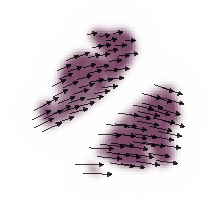
\includegraphics[height=\bbgeodesicpanelheight]{figures/dynamic-benamou-brenier-geodesic/midpoint-velocities.pdf}
\\[-.1em]
\small density sequence &
\small midpoint velocities
\end{tabular}
\caption{\emph{Benamou--Brenier geodesic between two sampled silhouettes.} A quadratic optimal plan induces the interpolation $Z_t=(1-t)X+tY$. Left: smoothed density snapshots along this least-action path. Right: shortened arrows at representative midpoint particles show the direction of the constant characteristic velocity $Y-X$.}
\index{McCann!interpolation}% strictindex
\label{fig:dynamic-benamou-brenier-geodesic}
\end{figure}

\paragraph{Path-space formulation.}\label{rem-bb-path-space}
\index{path-space formulation}% strictindex
	Let $\Ss=C([0,1];\RR^d)$ be the space of continuous paths endowed with the uniform topology. For $t\in[0,1]$ define the evaluation map
	\[
		e_t:\Ss\to\RR^d,
		\qquad
		e_t(\gamma)=\gamma(t).
	\]
	The Benamou--Brenier cost admits the equivalent formulation
\index{Benamou-Brenier@Benamou--Brenier}% strictindex
	\[
		\Wass_2^2(\alpha_0,\alpha_1)
		=
		\inf_{M\in\Pp(\Ss)}
		\enscond{
			\int_{\Ss}\!\int_0^1\norm{\dot\gamma(t)}^2\d t\,\d M(\gamma)
		}{
			(e_0)_\sharp M=\alpha_0,\ (e_1)_\sharp M=\alpha_1
		}.
	\]
	The inner kinetic energy is understood as $+\infty$ when $\gamma$ is not absolutely continuous. If $\alpha_0$ has a density, the minimizer $M^*$ is unique. Its time marginals reproduce the optimal curve: $\alpha_t=(e_t)_\sharp M^*$ for all $t$. Furthermore, for a.e.\ $t$, denoting $\dot e_t(\gamma)=\dot\gamma(t)$ on absolutely continuous paths, the conditional law of the velocity is deterministic:
\index{absolutely continuous path}% strictindex
\index{conditional!law}% strictindex
	\[
		(e_t,\dot e_t)_\sharp M^*(\d x,\d q)
		=
		\alpha_t(\d x)\delta_{v_t^*(x)}(\d q),
	\]
	where $v_t^*$ is the optimal velocity field in the Benamou--Brenier formulation. Hence $M^*$ concentrates on straight-line geodesics and, for a.e.\ $t$, assigns exactly one direction at $\alpha_t$-a.e.\ spatial point.
\index{Benamou-Brenier@Benamou--Brenier}% strictindex
\index{velocity field}% strictindex
\index{Benamou-Brenier@Benamou--Brenier!formulation}% strictindex

%%%%%%%%%%%%%%%%%%%%%%%%%%%%%%%%%%%%%%%%%%%%%%%%%%%%%%%%%%%%%%%%%%%%%%%%%%%

\paragraph{Beyond the quadratic transport action.}\label{par-generalized-dynamic-perspectives}
The Benamou--Brenier construction can be modified by changing either the cost of motion or the admissible ways of moving mass. Density-dependent mobilities model transport whose resistance varies with the local concentration~\citep{dolbeault2009new}. Edge fluxes and jump kernels replace local velocities on graphs or in nonlocal spaces~\citep{Maas2011,MielkeCVPDE,Erbar2012JumpEntropy}. Unbalanced transport adds creation and destruction of mass, giving the Wasserstein--Fisher--Rao or Hellinger--Kantorovich geometry~\citep{LieroMielkeSavareLong,2017-chizat-focm}. Variational mean field games keep the continuity constraint but add running congestion and terminal costs; for potential couplings, the resulting planning problem describes the equilibrium of a population of interacting agents~\citep{LasryLions2007MeanFieldGames,BenamouCarlierSantambrogio2017}. These extensions illustrate the flexibility of the least-action viewpoint. The following section develops the quadratic Wasserstein geometry in detail, because it supplies the common calculus for the learning and sampling models considered here.

\FloatBarrier

% !TEX root = ../PDE4ML.tex

\section{Wasserstein Gradient Flows}
\index{Wasserstein!gradient}% strictindex
\index{gradient!flow}% strictindex
\index{Wasserstein!gradient flow}% strictindex
\label{sec-wasserstein-gradient-flows}

Once $\Wass_2$ is understood as a dynamic metric, one can run gradient descent directly on the space of measures. This section derives Wasserstein gradients from minimizing movements, studies dissipation and convergence through geodesic convexity and slope inequalities, and applies the calculus to interacting particles and mean-field neural networks. The final application retains depth as a conditioning variable, giving the geometry appropriate for training continuous-depth residual networks.
\index{mean-field neural network}% strictindex
\index{minimizing movement}% strictindex
\index{convexity!geodesic}% strictindex
\index{JKO scheme}% strictindex

\subsection{Minimizing Movements and Wasserstein Gradients}
\index{minimizing movement}% strictindex
\index{Wasserstein!gradient}% strictindex

This first section explains how a variational implicit-Euler step on measures gives rise, in the small-step limit, to a continuity equation driven by the Wasserstein gradient of the energy.
\index{continuity equation}% strictindex

We now consider a function $f(\alpha)$ and seek a minimizing evolution $(\alpha_t)_t$. The general strategy is the following implicit Euler construction.
\index{implicit Euler scheme}% strictindex
\begin{defn}[JKO minimizing movement]\label{def-jko-minimizing-movement}
Given $\tau>0$ and $\alpha^{(0)}$, define recursively
\begin{equation}
    \alpha^{(\ell+1)} \in \uargmin{\alpha\in\Pp_2(\RR^d)}
    \left\{\frac{1}{2 \tau} \Wass_2(\alpha^{(\ell)}, \alpha)^2 + f(\alpha)\right\}. \label{eq:jko-discr}
\end{equation}
\end{defn}
The piecewise-constant interpolation is $\alpha_\tau(t)=\alpha^{(\ell)}$ for $t\in[\ell\tau,(\ell+1)\tau)$. A limiting curve as $\tau\downarrow0$, when it exists, is called a minimizing movement. Existence of each minimizer and convergence of the interpolations require assumptions on $f$; they are not part of the definition of the recursion.


\paragraph{Euclidean gradient flows.}
\index{gradient!flow}% strictindex

If we restrict \eqref{eq:jko-discr} to finite dimensions and assume $\alpha_t = \delta_{x(t)}$ and $\alpha = \delta_x$ (single Dirac measures), this matches the implicit Euler scheme:
\index{Dirac mass}% strictindex
\index{implicit Euler scheme}% strictindex
\begin{equation*}
    x(t+\tau) \in \uargmin{x}\left\{\frac{1}{2 \tau} \norm{x - x(t)}^2 + h(x)\right\},
\end{equation*}
where $h(x) = f(\delta_x)$. When $h$ is differentiable, every minimizer satisfies $x(t+\tau)+\tau\nabla h(x(t+\tau))=x(t)$. If $\Id+\tau\nabla h$ is invertible, as for a globally Lipschitz gradient and sufficiently small $\tau$, this becomes
\begin{equation*}
    x(t+\tau) = (\Id + \tau \nabla h)^{-1}(x(t)).
\end{equation*}
In contrast, the explicit Euler scheme is:
\begin{equation*}
    x(t+\tau) = (\Id - \tau \nabla h)(x(t)) = x(t) - \tau \nabla h(x(t)).
\end{equation*}

If, for instance, $\nabla h$ is globally Lipschitz, then for sufficiently small $\tau$ both schemes are well posed and their interpolants converge locally uniformly as $\tau\to0$ to the unique solution of
\begin{equation}
    \dot{x}(t) = -\nabla h(x(t)). \label{eq:grad-flow-classical}
\end{equation}
The same conclusion holds under local Lipschitz regularity when the discrete and continuous trajectories remain in a common bounded set. Differentiability alone is insufficient: if the ODE is nonunique, explicit and implicit discretizations can select different solutions.


\paragraph{Vertical derivative (first variation).}
\index{derivative!vertical}% strictindex
\index{first variation}% strictindex
\index{functional!derivative}% strictindex

Deriving a PDE from the JKO scheme requires distinguishing affine from transport perturbations. The mixture \(\alpha_\vartheta=(1-\vartheta)\alpha+\vartheta\beta\) changes mass without prescribing how particles move and defines the \emph{linear functional}, \emph{flat} or \emph{vertical} derivative. The horizontal derivative introduced below instead follows a transport displacement.
\index{first variation}% strictindex
\index{signed!measure}% strictindex
\begin{defn}[First variation]\label{def-first-variation}
	Assume that \(f(\alpha)<+\infty\). A measurable function \(\delta f(\alpha)\) is a first variation of \(f\) at \(\alpha\) if, for every \(\beta\in\Pp(\RR^d)\) such that \(\delta f(\alpha)\) is integrable with respect to \(\lvert\beta-\alpha\rvert\) and the mixture \(\alpha_\vartheta\) remains in the domain of \(f\) for small \(\vartheta>0\),
	\[
		f(\alpha_\vartheta)
		=
		f(\alpha)
		+\vartheta\int_{\RR^d}[\delta f(\alpha)](x)
		\d(\beta-\alpha)(x)
		+o(\vartheta)
		\qquad(\vartheta\downarrow0).
	\]
\end{defn}
Because \(\beta-\alpha\) has zero mass, adding a constant to \(\delta f(\alpha)\) does not change the first variation. With a sufficiently rich class of admissible perturbations, this is its only ambiguity. It represents the directional linear form
\[
	Df(\alpha)[\eta]
	\eqdef
	\int_{\RR^d}[\delta f(\alpha)](x)\d\eta(x)
\]
whenever the zero-mass signed perturbation \(\eta\) is admissible. For example, if \(f(\alpha)=\int V\,\d\alpha\), then \(\delta f(\alpha)=V\): the vertical derivative records the value \(V(x)\), whereas the horizontal derivative will record its spatial gradient \(\nabla V(x)\).

\paragraph{Horizontal derivative (Wasserstein gradient).}
\index{derivative!horizontal}% strictindex
\index{Wasserstein!gradient}% strictindex

The vertical derivative asks how \(f\) reacts when mass is reweighted. Wasserstein geometry asks how it reacts when mass is moved through a Lagrangian displacement \((\Id+\vartheta v)_\sharp\alpha\). When the first variation is differentiable in \(x\), its spatial gradient represents this horizontal differential, provided the corresponding transport chain rule is valid.

As \(\tau\to0\), under suitable conditions on \(f\), \eqref{eq:jko-discr} defines a continuous evolution \(t\mapsto\alpha_t\). As discussed earlier, this evolution can be described by the Lagrangian advection formula~\eqref{eq:lagrangian-advection}. The key infinitesimal object is the vector field representing the differential in the Wasserstein metric.

\begin{defn}[Wasserstein gradient]\label{def-wasserstein-gradient}
\index{Wasserstein!gradient}% strictindex
	Assume that $f$ admits a smooth first variation $\delta f(\alpha)$. Here smoothness means that $\nabla\delta f(\alpha)\in L^2(\alpha;\RR^d)$, that the transport chain rule holds along the admissible continuity-equation curves, and that the boundary conditions justify integration by parts. We also require this spatial gradient to belong to the Wasserstein tangent space defined in~\eqref{eq-wasserstein-tangent-space}. In the smooth formal calculus on $\Pp_2(\RR^d)$, the Wasserstein gradient of $f$ at $\alpha$ is the gradient vector field
	\begin{equation*}
	    \Wgrad f(\alpha) = \nabla_x \delta f(\alpha).
	\end{equation*}
\end{defn}



The associated formal gradient flow is the continuity equation
\begin{equation}
    \frac{\partial \alpha_t}{\partial t} + \diverg(-\Wgrad f(\alpha_t) \alpha_t) = 0. \label{eq:wassflow-pde}
\end{equation}
The following proposition explains why this vector field is the Riemannian gradient for the $L^2(\alpha)$ metric on velocities.
\index{signed!measure}% strictindex
%
\begin{proposition}[Formal Wasserstein gradient]\label{prop-formal-wass-gradient}
\index{Wasserstein!gradient}% strictindex
	Assume that $f$ admits a smooth first variation $\delta f(\alpha)$ and that $\alpha$ has a smooth positive density. Let $v$ be a sufficiently regular velocity field, compactly supported or satisfying a no-flux boundary condition. For perturbations generated by $(\Id+\tau v)_\sharp\alpha$, the differential of $f$ is
\index{first variation}% strictindex
\index{velocity field}% strictindex
	\[
		\frac{\d}{\d\tau}_{|\tau=0}
		f\big((\Id+\tau v)_\sharp\alpha\big)
		=
		\int \dotp{\nabla \delta f(\alpha)(x)}{v(x)}\d\alpha(x).
	\]
	Hence, for the Riemannian metric $\norm{v}_{L^2(\alpha)}^2=\int \norm{v}^2\d\alpha$, the Wasserstein gradient is the vector field
\index{Wasserstein!gradient}% strictindex
	\[
		\Wgrad f(\alpha)=\nabla \delta f(\alpha).
	\]
\end{proposition}
\begin{proof}
	The push-forward expansion gives, in the sense of distributions,
\index{push-forward}% strictindex
	\[
		(\Id+\tau v)_\sharp\alpha
		=
		\alpha-\tau\diverg(\alpha v)+o(\tau).
	\]
	In the smooth density case, write $\alpha=\rho\,\d x$. The first variation and the transport chain rule give
\index{first variation}% strictindex
	\[
		f((\Id+\tau v)_\sharp\alpha)
		=
		f(\alpha)-\tau\int \delta f(\alpha)\diverg(\rho v)\d x+o(\tau).
	\]
	An integration by parts, with either compact support or vanishing boundary flux, gives
\index{flux}% strictindex
	\[
		-\int \delta f(\alpha)\diverg(\rho v)\d x
		=
		\int \dotp{\nabla\delta f(\alpha)}{v}\d\alpha.
	\]
	For a general measure, the same identity is a distributional pairing, under the stated chain-rule assumptions. By definition of the Riesz representative on the Wasserstein tangent space, this representative is $\nabla\delta f(\alpha)$.
\end{proof}

The geometric viewpoint on densities has an early antecedent in Lafferty's density manifold~\citep{Lafferty1988DensityManifold}. Otto developed the formal Riemannian structure underlying Wasserstein gradient flows~\citep{otto2001geometry}. Rigorous metric-space treatments and numerical JKO schemes can be found in~\citet{ambrosio2006gradient,JDB-JKO,2015-Peyre-siims,gallouet2017jko}.
\index{Wasserstein!gradient}% strictindex
\index{Wasserstein!gradient flow}% strictindex
\index{JKO scheme}% strictindex

\paragraph{From the JKO step to the velocity field.}
\index{velocity field}% strictindex

A first-order expansion of the JKO step explains why~\eqref{eq:wassflow-pde} uses the vector field $\Wgrad f(\alpha)$. This is a formal local argument: assume that $\alpha_t$ is absolutely continuous and that, for the nearby competitors selected by the JKO step, the optimal map from $\alpha_t$ can be written as $\Id+\tau v$. For these optimal displacement representatives,
	\[
		\Wass_2^2\bigl(\alpha_t,(\Id+\tau v)_\sharp\alpha_t\bigr)
		=
		\tau^2\norm{v}_{L^2(\alpha_t)}^2.
	\]
The local JKO objective therefore reads
	\[
		\min_v \frac{\tau}{2}\norm{v}_{L^2(\alpha_t)}^2
		+f\bigl((\Id+\tau v)_\sharp\alpha_t\bigr),
	\]
where the minimization is restricted to these representatives. The two expansions
	\begin{align*}
		(\Id+\tau v)_\sharp\alpha_t
		&=
		\alpha_t-\tau\diverg(v\alpha_t)+o(\tau),\\
		f\bigl((\Id+\tau v)_\sharp\alpha_t\bigr)
		&=
		f(\alpha_t)
		+\tau\int\dotp{\nabla_x\delta f(\alpha_t)(x)}{v(x)}\d\alpha_t(x)
		+o(\tau)
	\end{align*}
give the first-order problem
	\[
		\min_v f(\alpha_t)
		+\tau\int\left[
			\frac12\norm{v(x)}^2
			+\dotp{\Wgrad f(\alpha_t)(x)}{v(x)}
		\right]\d\alpha_t(x)
		+o(\tau).
	\]
Its pointwise minimizer is $v=-\Wgrad f(\alpha_t)$, which gives the velocity in the continuity equation. A rigorous passage from the discrete scheme to a curve of maximal slope uses compactness and lower-semicontinuity rather than this formal parametrization; see~\citet{JDB-JKO,ambrosio2006gradient}.
\index{continuity equation}% strictindex

\paragraph{Metric derivative and curves of maximal slope.}
\index{metric!derivative}% strictindex
\index{curve of maximal slope}% strictindex
\index{metric slope}% strictindex
\index{metric slope!local}% strictindex

The same descent principle admits a coordinate-free formulation, which is the right language for limits of JKO schemes.
\begin{defn}[Metric derivative and absolutely continuous curve]\label{def-metric-derivative-ac-curve}
For \(1\leq p\leq+\infty\), a curve $x:[0,T]\to(\mathcal X,d)$ belongs to \(AC^p([0,T];\mathcal X)\) if some $g\in L^p(0,T)$ satisfies $d(x_s,x_t)\leq\int_s^t g(r)\d r$. Absolutely continuous means \(AC^1\). Its metric derivative is
		\[
		|\dot x_t|
		\eqdef
			\lim_{h\to 0}\frac{d(x_{t+h},x_t)}{|h|}
		\]
for a.e.\ $t$.
\end{defn}

Energy descent is encoded by the slope and its upper-gradient property.
\begin{defn}[Metric slope and curve of maximal slope]\label{def-curve-maximal-slope}
\index{metric slope}% strictindex
For lower-semicontinuous $f:\mathcal X\to(-\infty,+\infty]$, define
		\[
		|\partial f|(x)
		\eqdef
		\begin{cases}
		\limsup_{\substack{y\to x\\ y\neq x}}
			\dfrac{( f(x)-f(y) )_+}{d(x,y)}, & f(x)<+\infty,\\[.4em]
		+\infty, & f(x)=+\infty.
		\end{cases}
		\]
It is a strong upper gradient if $|f(y_t)-f(y_s)|\leq \int_s^t |\partial f|(y_r)|\dot y_r|\d r$ along every absolutely continuous $y$. When this property holds, a curve $x\in AC^2([0,T];\mathcal X)$ with $f(x_0)<+\infty$ is a curve of maximal slope for $f$ if $f\circ x$ has an absolutely continuous representative and
\index{strong upper gradient}% strictindex
\index{energy-dissipation inequality}% strictindex
	\[
		f(x_t)
		+\frac12\int_s^t |\dot x_r|^2\d r
		+\frac12\int_s^t |\partial f|^2(x_r)\d r
		\leq f(x_s),
			\qquad 0\leq s<t.
		\]
\end{defn}
This is the metric-space formulation of gradient descent~\citep{ambrosio2006gradient}; the inequality passes to limits when the energy and slope have the required lower-semicontinuity properties. With the strong-upper-gradient assumption in Definition~\ref{def-curve-maximal-slope}, it is necessarily saturated: the chain rule gives $-(f\circ x)'\leq |\partial f|(x)|\dot x|$, while the dissipation inequality gives the reverse bound by $(|\partial f|^2+|\dot x|^2)/2$. Equality in Young's inequality then yields $-(f\circ x)'=|\dot x|^2=|\partial f|^2(x)$ almost everywhere. In $\mathcal X=\Pp_2(\RR^d)$ with $d=\Wass_2$, an absolutely continuous curve admits a continuity-equation velocity $v_t$ and satisfies $|\dot\alpha_t|_{\Wass_2}\leq\norm{v_t}_{L^2(\alpha_t)}$, with equality for the minimal velocity. For smooth energies, $|\partial f|(\alpha_t)=\norm{\Wgrad f(\alpha_t)}_{L^2(\alpha_t)}$, so the maximal-slope condition reduces to the velocity-field equation $v_t=-\Wgrad f(\alpha_t)$ derived above. The energy consequences of this viewpoint are used below in Section~\ref{sec-geodesic-convexity}.
\index{minimal velocity}% strictindex

\begin{rem}[$\Wass_2$-Lipschitz functionals and bounded gradients]\label{rem-w2-lipschitz-bounded-gradient}
\index{Wasserstein!Lipschitz functional}% strictindex
\index{Wasserstein!gradient}% strictindex
	A functional is $L$-Lipschitz for $\Wass_2$ if $|f(\alpha)-f(\beta)|\leq L\Wass_2(\alpha,\beta)$ for all measures in its domain. An \(L\)-Lipschitz functional has descending metric slope at most \(L\). Conversely, on a geodesic metric space, if the slope is a strong upper gradient uniformly bounded by \(L\), integrating it along geodesics shows that the functional is \(L\)-Lipschitz. In the smooth Otto calculus, under the chain-rule assumptions used in Proposition~\ref{prop-formal-wass-gradient}, this slope is
	\[
		|\partial f|_{\Wass_2}(\alpha)
		=
		\norm{\Wgrad f(\alpha)}_{L^2(\alpha)}.
	\]
	Thus
	\[
		\sup_{\alpha}\norm{\Wgrad f(\alpha)}_{L^2(\alpha)}\leq L
	\]
	is the differential counterpart of \(\Wass_2\)-Lipschitz regularity.
\end{rem}

We now detail examples of such Wasserstein gradient flows.
\index{Wasserstein!gradient}% strictindex
\index{gradient!flow}% strictindex
\index{Wasserstein!gradient flow}% strictindex

\begin{example}[Application to single-cell gradient-flow models]\label{ex-single-cell-gradient-flow}
\index{single-cell genomics}% strictindex
\index{Waddington landscape}% strictindex
	Instead of only coupling successive snapshots, one may posit that a latent population law evolves by
	\[
		\partial_t\al_t+\diverg(\al_t v_t)=0,
		\qquad
		v_t=-\Wgrad f(\al_t)=-\nabla\delta f(\al_t).
	\]
	Here \(\delta f(\al_t)\) is the first variation, with the convention introduced above. For example, if \(\al=\rho\,\d x\), the energy \(f(\al)=\int V\d\al+\sigma^2\int\rho\log\rho\,\d x\) gives a drift toward a potential landscape \(V\) together with diffusion of strength \(\sigma^2\). In single-cell modeling, \(V\), interaction terms or a neural approximation of \(v_t\) can be fitted from unpaired population snapshots. This links Waddington-landscape intuition to the mathematical language of dynamic OT, Fokker--Planck equations and flow matching~\citep{TongHuangWolfVanDijkKrishnaswamy2020TrajectoryNet,LavenantZhangKimSchiebinger2021TrajectoryInference,KleinUsciddaTheisCuturi2023GENOT}.
\end{example}

Figure~\ref{fig:gradflow-jko-entropy-steps} shows the same minimizing-movement construction both in density coordinates and through the motion of quantiles.

\begin{figure}[htbp]
\centering
\begin{tabular}{@{}cc@{}}
\small density iterates & \small quantile motion \\[-.15em]
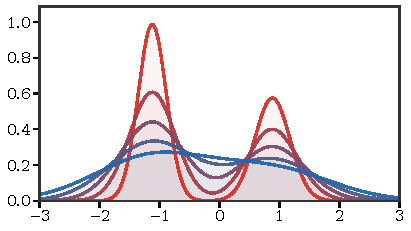
\includegraphics[width=.37\linewidth]{figures/gradflow-jko-entropy-steps/density-steps.pdf} &
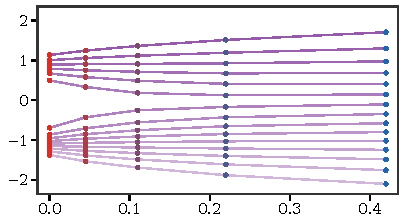
\includegraphics[width=.37\linewidth]{figures/gradflow-jko-entropy-steps/quantile-steps.pdf}
\end{tabular}
\caption{\emph{JKO minimizing movements for the entropy flow in one dimension.} The left panel displays successive implicit-Euler minimizers for the heat equation, colored from red to blue. The right panel tracks inverse CDF values $\cumul{\alpha_t}^{-1}(s)$ for selected probability levels $s$, giving a Lagrangian view of the proximal movement in Wasserstein space.}
\index{minimizing movement}% strictindex
\index{Wasserstein!space}% strictindex
\index{heat equation}% strictindex
\index{JKO scheme}% strictindex
\label{fig:gradflow-jko-entropy-steps}
\end{figure}

\paragraph{Discrete evolutions.}
\index{measure!evolution}% strictindex

If $f$ admits a first variation whose spatial gradient is well defined at empirical measures, the characteristic form of~\eqref{eq:wassflow-pde} admits a fixed-weight particle representation for as long as the characteristic ODE is well posed. Collisions can reduce the number of distinct support points. For equal weights, write $\alpha_t = \frac{1}{n} \sum_i \delta_{x_i(t)}$. The particles $X(t) := (x_i(t))_i$ evolve according to the coupled ODEs
\index{Dirac mass}% strictindex
\begin{equation}
    \dot{x}_i(t) = -n\nabla_{x_i} F(X(t)), \label{eq:wassflows-particles}
\end{equation}
where $F(X) := f\left(\frac{1}{n} \sum_i \delta_{x_i}\right)$ and the factor $n$ comes from the empirical Wasserstein metric $\frac1n\sum_i \norm{\dot x_i}^2$.


\paragraph{Linear functionals.}
\index{linear!functional}% strictindex

The first benchmark is a functional whose first variation does not depend on the current measure.

\begin{example}[Linear potentials generate independent particles]
\index{linear!potential}% strictindex
\eqllead{Take a linear functional}{eq:linear-func}{
       f(\alpha) = \int h(x) \d \alpha(x).
   }
   Then $\delta f(\alpha) = h$ is independent of $\alpha$, and the flow \eqref{eq:wassflow-pde} becomes
   \begin{equation*}
       \frac{\partial \alpha_t}{\partial t} + \diverg(-\nabla h \alpha_t) = 0.
   \end{equation*}
   This implies particles move independently according to the usual gradient flow \eqref{eq:grad-flow-classical}.
\index{gradient!flow}% strictindex
\end{example}

\paragraph{Shannon neg-entropy.}
\index{entropy!negative Shannon}% strictindex


Entropy gives the opposite benchmark: particles are no longer independent trajectories driven by a fixed vector field. The evolution is a diffusion, or formally a continuity equation with the density-dependent score velocity $-\nabla\log\rho_t$; when that velocity generates a sufficiently regular flow, the latter still provides a deterministic push-forward representation.

\begin{defn}[Score function]\label{def-score-function}
For $\alpha=\rho\,\d x$ with differentiable positive density $\rho$, its score is $\nabla\log\rho$. Relative to $\beta$, its relative score is $\nabla\log(\d\alpha/\d\beta)$ whenever this logarithmic density has a weak gradient.
\end{defn}

\begin{example}[Entropy generates heat and porous-medium flows]
The canonical density-dependent functional is the Shannon neg-entropy
   \begin{equation}
       f(\alpha) = \int \log\left(\frac{\d \alpha}{\d x}(x)\right) \d \alpha(x). \label{eq:entropy-func}
   \end{equation}
	   If $\alpha=\rho\d x$, then $\delta f(\alpha) = \log\rho+1$, up to an immaterial additive constant, so $\Wgrad f(\alpha) = \nabla\log\rho$ is the score. The flow \eqref{eq:wassflow-pde} becomes the heat equation
\index{score function}% strictindex
\index{heat equation}% strictindex
   \begin{equation*}
	       \partial_t \rho_t = \Delta \rho_t.
   \end{equation*}
   Other entropy functionals lead to nonlinear diffusion equations; finite-volume and particle discretizations are discussed in~\citet{CarrilloFiniteVolume,GianazzaARMA,Maas2011,ErbarHeatManifold}.
%
\eqllead{For a generalized entropy}{eq:gen-entropies}{
	       f(\rho\d x) = \int g(\rho(x)) \d x,
   }
	   with a scalar convex function $g$, one obtains nonlinear diffusions in the smooth-density regime:
\index{convex!function}% strictindex
   \begin{equation*}
	       \frac{\partial \rho_t}{\partial t} = \Delta(P(\rho_t)),
   \end{equation*}
   where the pressure $P$ satisfies $P'(s)=s g''(s)$. For example, $g(s) = s \log(s)$ gives $P(s)=s$ and recovers \eqref{eq:entropy-func}, while $g(s) = s^m/(m-1)$, $m > 1$, gives $P(s)=s^m$ up to an additive constant and yields the porous-medium equation.
\index{porous medium equation}% strictindex
\end{example}

\begin{rem}[Two gradient-flow interpretations of the heat equation]\label{rem-two-interpretations-heat-equation}
\index{heat equation}% strictindex
\index{Dirichlet energy}% strictindex
\index{gradient!flow}% strictindex
\index{entropy!Shannon}% strictindex
\index{Wasserstein!gradient flow}% strictindex
	The heat equation already illustrates that a PDE does not determine a unique gradient-flow structure. Write $\alpha=\rho\d x$ on a flat domain, with periodic or no-flux boundary conditions. In the Hilbert geometry of densities, the squared distance and the Dirichlet energy are
	\[
		d_{L^2}^2(\alpha,\beta)=\int |\rho_\alpha(x)-\rho_\beta(x)|^2\d x,
		\qquad
		\mathcal D(\alpha)=\frac12\int \norm{\nabla\rho(x)}^2\d x,
	\]
	so $\delta\mathcal D/\delta\rho=-\Delta\rho$ and the $L^2$ gradient flow $\partial_t\rho_t=-\delta\mathcal D/\delta\rho(\rho_t)$ gives $\partial_t\rho_t=\Delta\rho_t$. This viewpoint says that heat flow decreases oscillations and regularizes the density. In Wasserstein geometry, the same equation is instead the $\Wass_2$ gradient flow of the Shannon entropy $\int \rho\log\rho\d x$, so the driving mechanism is entropic spreading. The example is a useful warning: explaining a dynamics as a gradient flow requires specifying both an energy and a metric, and different pairs $(f,d)$ may produce the same PDE.
\end{rem}

Figure~\ref{fig:gradflow-heat-versus-porous-medium} contrasts the spreading induced by the linear heat equation with the compactly supported, density-dependent propagation of two porous-medium flows.

\begin{figure}[ht]
\centering
\begin{tabular}{@{}ccc@{}}
\small heat equation & \small porous medium $m=2$ & \small porous medium $m=6$ \\[-.15em]
\index{heat equation}% strictindex
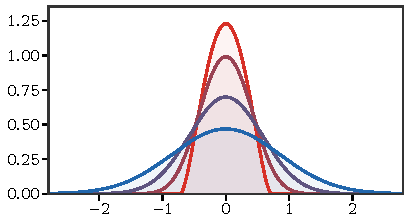
\includegraphics[width=.30\linewidth]{figures/gradflow-heat-versus-porous-medium/heat.pdf} &
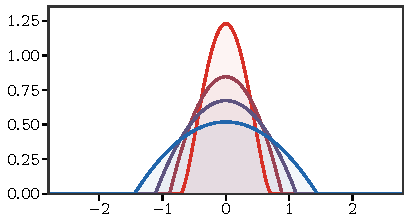
\includegraphics[width=.30\linewidth]{figures/gradflow-heat-versus-porous-medium/porous-medium.pdf} &
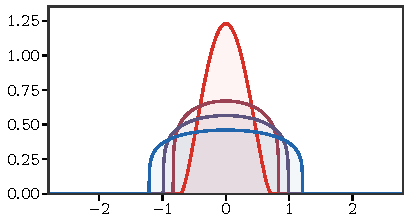
\includegraphics[width=.30\linewidth]{figures/gradflow-heat-versus-porous-medium/porous-medium-m6.pdf}
\end{tabular}
\caption{\emph{Entropy-driven Wasserstein gradient flows from the same compact initial density.} The heat flow is generated by Shannon entropy $g(\rho)=\rho\log\rho$ and instantly develops Gaussian tails. The porous-medium flows use the power entropy $g(\rho)=\rho^m/(m-1)$, hence $\partial_t\rho=\Delta(\rho^m)$: the middle panel has $m=2$, while the right panel has the stronger nonlinearity $m=6$, i.e.\ $\partial_t\rho=\Delta(\rho^6)$. Larger powers diffuse mainly where the density is high, producing a flatter core and a sharper compact free boundary.}
\index{Wasserstein!gradient flow}% strictindex
\index{entropy!Shannon}% strictindex
\label{fig:gradflow-heat-versus-porous-medium}
\end{figure}

\paragraph{Interaction energies.}
\index{energy!interaction}% strictindex

In a similar spirit, to obtain nonlinear evolutions without requiring the measure to have density, one can consider
   \begin{equation}
       f(\alpha) := \iint k(x, y) \d \alpha(x) \d \alpha(y). \label{eq:quadratic-func}
   \end{equation}
   For a symmetric differentiable kernel $k$, assuming the displayed integrals and derivatives exist:
   \begin{equation*}
       \delta f(\alpha)(x) = 2 \int k(x, y) \d \alpha(y), \quad \Wgrad f(\alpha)(x) = 2 \int \nabla_x k(x, y) \d \alpha(y).
   \end{equation*}
   For $\alpha_0 = \frac{1}{n} \sum_i \delta_{x_i}$, the flow \eqref{eq:wassflow-pde} implies particles $(x_i(t))_i$ obey:
   \begin{equation*}
       \dot{x}_i(t) = -\frac{2}{n} \sum_j \nabla k(x_i(t), x_j(t)).
   \end{equation*}
	   If $k$ is positive semidefinite, or more generally conditionally positive semidefinite on signed measures of zero total mass as for the energy-distance kernel $k(x,y)=-\norm{x-y}$, and one minimizes the squared kernel discrepancy to a teacher distribution $\beta$, then
\index{teacher distribution}% strictindex
\index{energy distance}% strictindex
\index{signed!measure}% strictindex
   \[
       \MMD_k^2(\alpha,\beta)
       =
       \iint k\d\alpha\d\alpha
       -2\int\!\left(\int k(x,y)\d\beta(y)\right)\d\alpha(x)
       +\mathrm{constant}.
       \]
	       Thus MMD-type training energies are exactly an interaction energy plus a linear potential; the teacher distribution appears through the potential $x\mapsto-2\int k(x,y)\d\beta(y)$. For a differentiable kernel, with differentiation under the integral justified, the corresponding empirical Wasserstein gradient flow is
\index{teacher distribution}% strictindex
\index{Wasserstein!gradient}% strictindex
\index{gradient!flow}% strictindex
\index{maximum mean discrepancy}% strictindex
\index{Wasserstein!gradient flow}% strictindex
\index{energy!interaction}% strictindex
       \[
		\dot x_i(t)
		=
		-\frac{2}{n}\sum_j\nabla_x k(x_i(t),x_j(t))
		+
		2\int\nabla_x k(x_i(t),y)\d\beta(y).
       \]



	       For $k(x,y)=-\norm{x-y}$, the kernel is not differentiable on the diagonal: its constant diagonal self-energy contributes zero, and distinct-particle collisions require a nonsmooth interpretation or regularization. These fixed-weight particle dynamics should not be confused with an unrestricted Wasserstein flow of the nonsmooth energy at an atomic law, which may lower its energy by splitting atoms. The first term is a kernelized self-interaction, while the second is the attraction induced by the continuous teacher kernel mean. At the continuum level, characteristic positive semidefinite kernels, and the Euclidean energy-distance kernel on laws with finite first moment, have $\beta$ as the unique minimizer of $\MMD_k^2(\alpha,\beta)$. For a finite number of particles, however, the flow can only form a kernelized quadrature of $\beta$, and small particle systems may cover the target modes poorly. Figure~\ref{fig:gradflow-mmd-particle-count} illustrates this finite-particle effect.
\index{kernelized self-interaction}% strictindex
\index{teacher kernel mean}% strictindex
\index{kernel!characteristic}% strictindex
\index{kernel!quadrature}% strictindex
\index{probability measure}% strictindex
\index{kernel!positive definite}% strictindex
\index{energy distance}% strictindex

\begin{figure}[ht]
\centering
\begin{tabular}{@{}ccc@{}}
\small $n=10$ particles & \small $n=50$ particles & \small $n=300$ particles \\[-.15em]
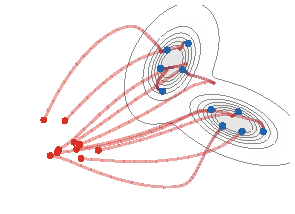
\includegraphics[width=.30\linewidth]{figures/gradflow-mmd-particle-count/n-010.pdf} &
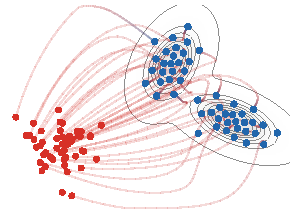
\includegraphics[width=.30\linewidth]{figures/gradflow-mmd-particle-count/n-050.pdf} &
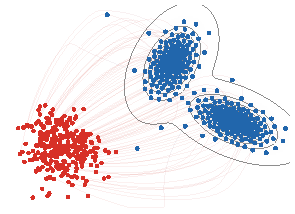
\includegraphics[width=.30\linewidth]{figures/gradflow-mmd-particle-count/n-300.pdf}
\end{tabular}
\caption{\emph{Particle count in an energy-distance Wasserstein particle flow.} The squared MMD-type discrepancy uses the energy-distance kernel $k(x,y)=-\norm{x-y}$ and targets a smooth two-Gaussian teacher distribution. The teacher itself is shown only through true density contours, while red dots are a compact shifted Gaussian initialization placed away from the target, red-to-blue curves show a thinned subset of particle trajectories, and blue dots show the stabilized long-time particles. With too few particles, the empirical measure forms a sparse kernelized quadrature and may under-cover the target modes; increasing $n$ makes the particle cloud approximate the continuous target geometry more faithfully.}
\index{teacher distribution}% strictindex
\index{kernel!quadrature}% strictindex
\index{Wasserstein!gradient flow}% strictindex
\index{empirical!measure}% strictindex
\index{energy distance}% strictindex
\label{fig:gradflow-mmd-particle-count}
\end{figure}

The preceding particle flow minimizes a squared kernel discrepancy. Figure~\ref{fig:gradflow-discrepancy-density-comparison} contrasts this with flows generated by three discrepancies toward the same target. For the energy distance and $\Wass_2$, the energy is the unsquared distance, so the Wasserstein velocity is normalized by the current discrepancy value away from the target. The KL case is different: it is a relative-entropy gradient flow and therefore follows the Fokker--Planck diffusion toward the target. The comparison keeps the endpoint fixed and makes the geometry visible through the transient densities.

\begin{figure}[ht]
\centering
\begin{tabular}{@{}ccc@{}}
\small energy distance & \small $\Wass_2$ distance & \small relative entropy \\[-.15em]
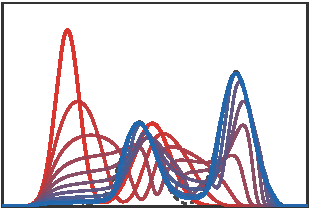
\includegraphics[width=.30\linewidth]{figures/gradflow-discrepancy-density-comparison/energy-distance.pdf} &
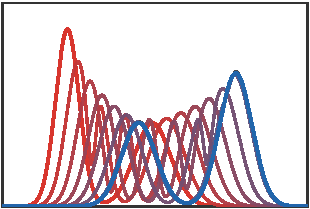
\includegraphics[width=.30\linewidth]{figures/gradflow-discrepancy-density-comparison/w2.pdf} &
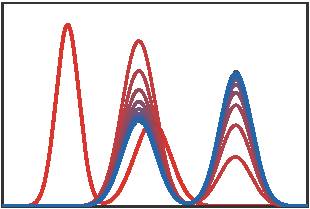
\includegraphics[width=.30\linewidth]{figures/gradflow-discrepancy-density-comparison/kl.pdf}
\end{tabular}
\caption{\emph{Wasserstein gradient flows of three discrepancies toward the same one-dimensional Gaussian-mixture target, shown as a dashed black density.} The source density is also a Gaussian mixture. Red-to-blue curves are snapshots of $\alpha_t$. The energy-distance and $\Wass_2$ panels descend the unsquared distances and use many equal-weight quantile particles: in one dimension the energy distance is obtained from $\MMD_{-|\cdot-\cdot|}^2(\alpha,\beta)=2\int |\cumul\alpha-\cumul\beta|^2\d x$, while $\Wass_2$ uses monotone quantile matching. The relative-entropy panel solves the reversible Fokker--Planck equation $\partial_t\rho=\partial_x(\rho_\beta\,\partial_x(\rho/\rho_\beta))$ by an implicit finite-volume scheme, so that $\rho_\beta$ is the discrete stationary density.}
\index{energy distance}% strictindex
\index{Kullback-Leibler@Kullback--Leibler!divergence}% strictindex
\index{Fokker-Planck@Fokker--Planck!equation}% strictindex
\index{Wasserstein!gradient flow}% strictindex
\label{fig:gradflow-discrepancy-density-comparison}
\end{figure}

Figure~\ref{fig:gradflow-interaction-particles} complements this target-matching example by isolating three self-interaction regimes.

\begin{figure}[ht]
\centering
\begin{tabular}{@{}ccc@{}}
\small repulsive kernel & \small attractive kernel & \small attraction--repulsion \\[-.15em]
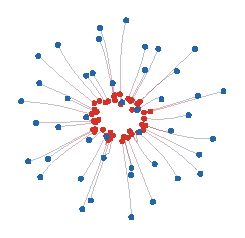
\includegraphics[width=.30\linewidth]{figures/gradflow-interaction-particles/repulsive.pdf} &
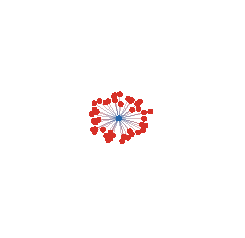
\includegraphics[width=.30\linewidth]{figures/gradflow-interaction-particles/attractive.pdf} &
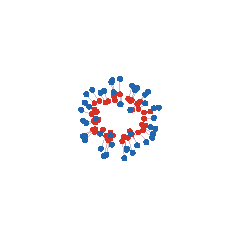
\includegraphics[width=.30\linewidth]{figures/gradflow-interaction-particles/attraction-repulsion.pdf}
\end{tabular}
\caption{\emph{Interaction-energy particle flows for three choices of $k$.} A positive Gaussian kernel $k(x,y)=\exp(-\norm{x-y}^2/(2\sigma^2))$ produces short-range repulsion under Wasserstein descent; changing its sign produces attraction and collapse; adding a quadratic long-range attraction to the repulsive kernel yields a balanced attraction--repulsion dynamics. The curves use arclength-based red-to-blue coloring along a longer integration of the coupled particle ODE~\eqref{eq:wassflows-particles}.}
\index{particle ODE}% strictindex
\index{energy!interaction}% strictindex
\label{fig:gradflow-interaction-particles}
\end{figure}

Figure~\ref{fig:gradflow-particle-objective-geometries} compares OT and MMD trajectories on common source and target clouds, and previews the prescribed drifting field introduced in Section~\ref{sec-one-step-generative-models}.

\begin{figure}[ht]
\centering
\begin{tabular}{@{}ccc@{}}
\small OT rays & \small MMD force & \small drifting field \\[-.15em]
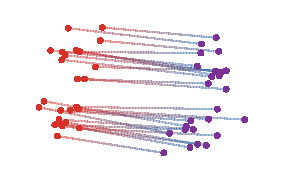
\includegraphics[width=.28\linewidth]{figures/gradflow-particle-objective-geometries/ot-rays.pdf} &
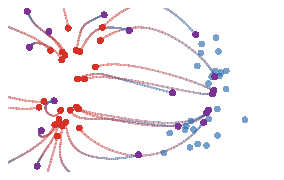
\includegraphics[width=.28\linewidth]{figures/gradflow-particle-objective-geometries/mmd-force.pdf} &
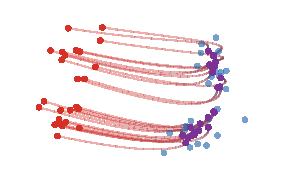
\includegraphics[width=.28\linewidth]{figures/gradflow-particle-objective-geometries/drifting-field.pdf}
\end{tabular}
\caption{\emph{Particle trajectories under transport, kernel and prescribed drifting fields.} The red particles and blue target cloud are the same in all panels. OT gives straight rays from an optimal matching; the MMD witness field couples particles through a kernel; and the normalized drifting field combines attraction to data with self-repulsion. The comparison concerns trajectory geometry, not solver performance.}
\label{fig:gradflow-particle-objective-geometries}
\end{figure}

\paragraph{Stochastic particles and McKean--Vlasov limits.}
\index{stochastic!particle}% strictindex
\index{McKean-Vlasov@McKean--Vlasov!limit}% strictindex
\index{McKean-Vlasov@McKean--Vlasov!equation}% strictindex
More generally, deterministic particle flows have stochastic counterparts, where Brownian noise at the particle level becomes an entropy term at the level of measures. Here $B_t$ denotes standard $d$-dimensional Brownian motion, and $\sigma>0$ sets the noise strength; the SDEs below are understood in the It\^o sense. If the drift does not depend on the empirical measure, each particle evolves independently according to
\index{empirical!measure}% strictindex
\[
	\d X_t=b(X_t)\d t+\sqrt{2}\sigma\d B_t,
\]
and the one-particle law $\alpha_t=\rho_t\d x$ directly satisfies the linear Fokker--Planck equation
\index{Fokker-Planck@Fokker--Planck!equation}% strictindex
\[
	\partial_t\rho_t=-\diverg(b\rho_t)+\sigma^2\Delta\rho_t.
\]

\begin{example}[Langevin drift as a free-energy flow]
\index{Langevin!free energy}% strictindex
	If $b=-\nabla V$, this linear Fokker--Planck equation is the $\Wass_2$ gradient flow of the free energy
	\[
		\rho\mapsto \int V\rho\,\d x+\sigma^2\int\rho\log\rho\,\d x.
	\]
\end{example}

The mean-field case is different: the drift is recomputed from the current empirical distribution of all particles,
\index{empirical!distribution}% strictindex
\index{gradient!flow}% strictindex
\index{mean-field limit}% strictindex
\[
	\d X_i^n(t)=b(X_i^n(t),\al_t^n)\d t+\sqrt{2}\sigma\d B_i(t),
	\qquad
	\al_t^n=\frac1n\sum_{i=1}^n\delta_{X_i^n(t)}.
\]
The Brownian motions $B_i$ are independent, and the initial particles are independent samples from a common law, independently of the noises. For finite $n$, the empirical law $\al_t^n$ is itself random. Under suitable Lipschitz, growth and chaotic-initialization assumptions, propagation of chaos states that finitely many particles become asymptotically independent as $n\to\infty$, all with the same deterministic law $\rho_t\d x$; equivalently, the empirical measure $\al_t^n$ converges in probability to this law. The limiting density solves the nonlinear Fokker--Planck, or McKean--Vlasov, equation
\index{Fokker-Planck@Fokker--Planck!equation}% strictindex
\index{McKean-Vlasov@McKean--Vlasov!limit}% strictindex
\index{propagation of chaos}% strictindex
\index{empirical!law}% strictindex
\index{McKean-Vlasov@McKean--Vlasov!equation}% strictindex
\[
	\partial_t \rho_t
	=
	-\diverg\big(b(x,\rho_t)\rho_t\big)
	+
	\sigma^2\Delta\rho_t.
\]
When the interaction drift is generated by an energy $f_0$ with variational form
\[
	b(x,\rho)=-\nabla[\delta f_0(\rho\,\d x)](x),
\]
	this PDE is the Wasserstein gradient flow of the entropy-regularized energy
\index{Wasserstein!gradient}% strictindex
\index{gradient!flow}% strictindex
\index{Wasserstein!gradient flow}% strictindex
	\[
		f(\rho\,\d x)=f_0(\rho\,\d x)+\sigma^2\int \rho\log\rho\,\d x.
	\]

For a prescribed target $\beta=\rho_\beta\d x$, take $b=\sigma^2\nabla\log\rho_\beta$. The SDE, the Fokker--Planck equation, and the deterministic continuity equation with score velocity are then three representations of the same gradient flow of $\sigma^2\KL(\cdot\mid\beta)$:
\begin{equation}\label{eq-relative-entropy-three-representations}
	\partial_t\rho_t
	=
	\sigma^2\diverg\!\left(\rho_t\nabla\log\frac{\rho_t}{\rho_\beta}\right),
	\qquad
	v_t
	=
	\sigma^2\bigl(\nabla\log\rho_\beta-\nabla\log\rho_t\bigr).
\end{equation}
Figure~\ref{fig:gradflow-fokker-planck-three-representations} compares numerical realizations of precisely these three descriptions.

\begin{figure}[ht]
\centering
\begin{tabular}{@{}c@{}}
\small independent Langevin particles \\[-.15em]
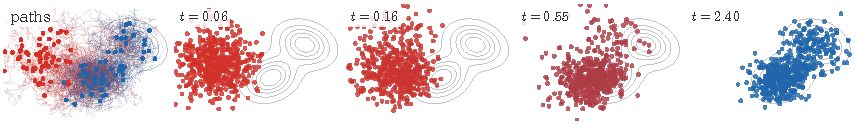
\includegraphics[width=.78\linewidth]{figures/gradflow-fokker-planck-three-representations/langevin-particles.pdf} \\[.25em]
\small deterministic KDE-score particles \\[-.15em]
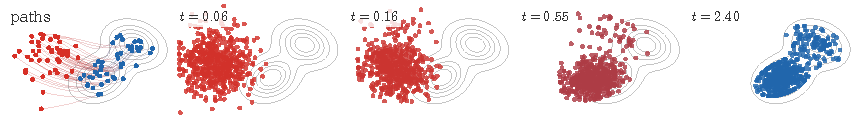
\includegraphics[width=.78\linewidth]{figures/gradflow-fokker-planck-three-representations/kde-particles.pdf} \\[.25em]
\small grid Fokker--Planck density \\[-.15em]
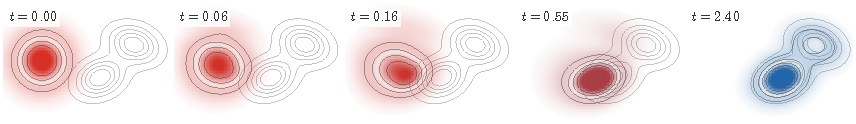
\includegraphics[width=.78\linewidth]{figures/gradflow-fokker-planck-three-representations/grid-pde.pdf}
\end{tabular}
\caption{\emph{Three numerical representations of an entropy-regularized Wasserstein gradient flow.} The target $\beta$ is a two-Gaussian density shifted to the right of an initially isotropic Gaussian density. The first row simulates independent Langevin particles and displays a thinned set of trajectories in the left panel. The second row evolves many deterministic particles with the score velocity in~\eqref{eq-relative-entropy-three-representations}, estimating $\nabla\log\rho_t$ by a kernel-density estimator; only representative trajectories and particle subsets are displayed. The third row solves the corresponding Fokker--Planck equation on a grid, starting from the initial density in the left panel. The remaining columns use front-loaded times, so that the onset of the flow and the later deformation toward a bimodal law are both visible.}
\index{Wasserstein!gradient flow}% strictindex
\index{Fokker-Planck@Fokker--Planck!equation}% strictindex
\index{Langevin!dynamics}% strictindex
\label{fig:gradflow-fokker-planck-three-representations}
\end{figure}


\subsection{Geodesic Convexity and Convergence}
\index{convexity!geodesic}% strictindex
\label{sec-geodesic-convexity}

Geodesic convexity is the convexity notion adapted to Wasserstein geometry. It is the condition that turns the formal gradient-flow calculus into a convergence theory.
\index{gradient!flow}% strictindex
\index{convexity!geodesic}% strictindex

\paragraph{Geodesics and convexity.}

A constant-speed $\Wass_2$ geodesic between $\alpha_0$ and $\alpha_1$ is obtained, as in Definition~\ref{def-w2-geodesic-induced-by-plan}, from any optimal coupling $\pi^\star\in\Couplings(\alpha_0,\alpha_1)$ by the McCann interpolation
\index{optimal coupling}% strictindex
\index{constant-speed geodesic}% strictindex
\index{McCann!interpolation}% strictindex
\[
	\alpha_t=((1-t)P_0+tP_1)_\sharp\pi^\star,
	\qquad t\in[0,1],
\]
where $P_0(x,y)=x$ and $P_1(x,y)=y$. If the optimal plan is induced by a Brenier map $T$, this reduces to $((1-t)\Id+tT)_\sharp\alpha_0$. The coupling formula is important because geodesics exist even when no Monge map exists, for instance when a Dirac mass must split.
\index{Monge!problem}% strictindex
\index{optimal coupling}% strictindex
\index{Brenier!map}% strictindex
\index{Dirac mass}% strictindex

\Needspace{9\baselineskip}
\begin{defn}[Geodesic convexity]\label{def-geodesic-convexity}
\index{convexity!geodesic}% strictindex
	A functional $f$ on $\Pp_2(\RR^d)$ is geodesically convex if for every $\Wass_2$ geodesic $(\alpha_t)_t$,
	\[
		f(\alpha_t)\leq (1-t)f(\alpha_0)+t f(\alpha_1).
	\]
	It is $\lambda$-geodesically convex if the right-hand side is improved by $-\frac{\lambda}{2}t(1-t)\Wass_2^2(\alpha_0,\alpha_1)$.
\end{defn}

\begin{prop}[Geodesic convexity of linear and quadratic energies]\label{prop-basic-geodesic-convexity}
\index{convexity!geodesic}% strictindex
	The following statements hold on the finite-energy domains of the displayed functionals in $\Pp_2(\RR^d)$, whenever their integrals are well defined.
	\begin{enumerate}
		\item If $h$ is convex, then the linear energy $\alpha\mapsto\int h\d\alpha$ is geodesically convex; if $h$ is $\lambda$-strongly convex, it is $\lambda$-geodesically convex. Conversely, if this linear energy is geodesically convex for all Dirac endpoints, then $h$ is convex.
		\item More generally, let \(k\geq2\) and let \(H_k:(\RR^d)^k\to\RR\cup\{+\infty\}\) be convex. Then the polynomial energy
		\[
			\alpha\mapsto \int_{(\RR^d)^k} H_k(x_1,\ldots,x_k)\,\d\alpha(x_1)\cdots\d\alpha(x_k)
		\]
		is geodesically convex whenever the integral is well defined. If $H_k$ is $\lambda$-strongly convex on the product space, this energy is $k\lambda$-geodesically convex. In particular, the quadratic interaction
		\[
			\alpha\mapsto\frac12\iint W(x,y)\d\alpha(x)\d\alpha(y)
		\]
		is geodesically convex when \(W\) is convex on \(\RR^d\times\RR^d\), and it is $\lambda$-geodesically convex when $W$ is $\lambda$-strongly convex there.
\index{energy!interaction}% strictindex
	\end{enumerate}
\end{prop}
\begin{proof}
	Let \(\pi\) be an optimal coupling between \(\alpha_0\) and \(\alpha_1\), and set \(X_t=(1-t)X_0+tX_1\) under \((X_0,X_1)\sim\pi\). Convexity of \(h\) gives \(h(X_t)\leq(1-t)h(X_0)+t h(X_1)\), and strong convexity gives the additional term \(-\frac{\lambda}{2}t(1-t)\norm{X_0-X_1}^2\). Integrating proves the first claim. Necessity follows by testing on Dirac masses: the geodesic between \(\delta_x\) and \(\delta_y\) is \(\delta_{(1-t)x+ty}\), so geodesic convexity of \(\int h\d\alpha\) gives the usual convexity inequality for \(h\).

	For the polynomial statement, take \(k\) independent copies \((X_0^\ell,X_1^\ell)_{\ell=1}^k\) of the same optimal coupling and define \(X_t^\ell=(1-t)X_0^\ell+tX_1^\ell\). Convexity of \(H_k\) on the product space gives
	\[
		H_k(X_t^1,\ldots,X_t^k)
		\leq (1-t)H_k(X_0^1,\ldots,X_0^k)+tH_k(X_1^1,\ldots,X_1^k).
	\]
	Integrating over the product coupling proves the claim. If $H_k$ is $\lambda$-strongly convex, the additional term is
	\[
		-\frac{\lambda}{2}t(1-t)
		\sum_{\ell=1}^k\EE\norm{X_0^\ell-X_1^\ell}^2
		=
		-\frac{k\lambda}{2}t(1-t)\Wass_2^2(\alpha_0,\alpha_1),
	\]
	which proves the stated constant. For the quadratic interaction, the prefactor $1/2$ cancels the factor $k=2$, leaving the constant $\lambda$.
\index{convexity!geodesic}% strictindex
\index{Monge!geodesic}% strictindex
\end{proof}

The polynomial criterion is useful but restrictive for kernel losses. The RKHS/MMD kernels introduced in Section~\ref{sec-rkhs-mmd} are usually chosen for positive definiteness and statistical smoothing, not for convexity as functions of \((x,y)\). Gaussian and Laplace kernels, for instance, are not convex on \(\RR^d\times\RR^d\), so positive definiteness of \(k\) does not imply that \(\alpha\mapsto\MMD_k^2(\alpha,\beta)\) is geodesically convex. In fact, such MMD losses are not geodesically convex in general. One-dimensional monotone transport gives a sharper exception for distance-type kernels, because ordered quantiles keep the sign of pairwise differences fixed along geodesics; this is the one-dimensional displacement-convexity mechanism emphasized, for instance, in~\citet{SantambrogioBook}.
\index{maximum mean discrepancy}% strictindex
\index{kernel!norm}% strictindex
\index{convexity!geodesic}% strictindex

\begin{prop}[One-dimensional interactions and energy-distance MMD]\label{prop-1d-interaction-halfline-convex}
\index{one-dimensional!transport}% strictindex
\index{convexity!geodesic}% strictindex
	Let \(\varphi:\RR_+\to\RR\) be continuous with at most quadratic growth, and define on \(\Pp_2(\RR)\)
	\[
		\mathcal I_\varphi(\alpha)
		\eqdef
		\frac12\iint \varphi(|x-y|)\d\alpha(x)\d\alpha(y).
	\]
	Then \(\mathcal I_\varphi\) is geodesically convex for \(\Wass_2\) on \(\Pp_2(\RR)\) if and only if \(\varphi\) is convex on \(\RR_+\).

	Fix also \(\beta\in\Pp_2(\RR)\). For the conditionally positive kernel \(k(x,y)=-|x-y|\) from Definition~\ref{def-positive-kernels}, the squared MMD of Definition~\ref{def-kernel-mmd-norm}, equivalently the squared energy distance,
	\[
		\mathcal E_\beta(\alpha)
		\eqdef
		\MMD_k^2(\alpha,\beta)
		=
		\iint -|x-y|\,\d(\alpha-\beta)(x)\d(\alpha-\beta)(y),
	\]
	is geodesically convex as a function of \(\alpha\).
\end{prop}
\begin{proof}
	Let \(Q_0,Q_1\) be the quantile functions of \(\alpha_0,\alpha_1\), and let \(Q_t=(1-t)Q_0+tQ_1\) be the quantile function of the one-dimensional \(\Wass_2\) geodesic \(\alpha_t\). For \(r>s\), monotonicity gives \(Q_i(r)-Q_i(s)\geq0\) for \(i=0,1\), and hence
	\[
		Q_t(r)-Q_t(s)
		=
		(1-t)(Q_0(r)-Q_0(s))+t(Q_1(r)-Q_1(s)).
	\]
	Using the symmetry of the double integral and the quantile parametrization, one can write
	\[
		\mathcal I_\varphi(\alpha_t)
		=
		\int_0^1\int_0^r
		\varphi(Q_t(r)-Q_t(s))\,\d s\,\d r.
	\]
	Convexity of \(\varphi\) on \(\RR_+\) gives the desired convexity after integration.

	Conversely, test geodesic convexity on two-point measures \(\alpha_i=\frac12(\delta_0+\delta_{a_i})\), with \(a_i\geq0\). Their monotone geodesic is \(\alpha_t=\frac12(\delta_0+\delta_{(1-t)a_0+t a_1})\). Since
	\[
		\mathcal I_\varphi(\alpha_t)
		=
		\frac14\varphi(0)+\frac14\varphi((1-t)a_0+t a_1),
	\]
	and the identical \(\frac14\varphi(0)\) terms cancel from the geodesic-convexity inequality, one obtains the ordinary convexity inequality for \(\varphi\) on \(\RR_+\).

	For the energy distance, the function \(\varphi(r)=-r\) is affine on \(\RR_+\), so the self-interaction \(-\iint |x-y|\d\alpha(x)\d\alpha(y)\) is affine along one-dimensional Wasserstein geodesics even though \(z\mapsto-|z|\) is not convex on \(\RR\). Write \(Q_\beta\) for the quantile function of \(\beta\). Expanding the MMD and dropping the term depending only on \(\beta\) gives
	\[
		\mathcal E_\beta(\alpha)
		=
		2\int_0^1\!\!\int_0^1 |Q_\alpha(r)-Q_\beta(s)|\,\d r\,\d s
		-
		\int_0^1\!\!\int_0^1 |Q_\alpha(r)-Q_\alpha(s)|\,\d r\,\d s
		+\mathrm{constant}.
	\]
	Here the constant is independent of \(\alpha\). The positive cross-distance term is convex in \(Q_\alpha\), since the absolute value is convex and \(Q_t\) is affine in \(t\). The self-distance term is affine along quantile geodesics because
	\[
		\int_0^1\!\!\int_0^1 |Q_t(r)-Q_t(s)|\,\d r\,\d s
		=
		2\int_0^1\int_0^r (Q_t(r)-Q_t(s))\,\d s\,\d r.
	\]
	Thus \(\alpha\mapsto\mathcal E_\beta(\alpha)\) is geodesically convex.
\index{maximum mean discrepancy}% strictindex
\index{energy distance}% strictindex
\end{proof}

This one-dimensional result is the mechanism behind the favorable behavior of energy-distance particle flows discussed earlier in this section and in recent analyses of distance-kernel MMD flows~\citep{DuongRuxSteinSteidl2024DistanceMMD}. It should not be read as a general MMD statement: for a typical positive definite kernel \(k\), the decomposition
\[
	\MMD_k^2(\alpha,\beta)
	=
	\iint k\,\d\alpha\d\alpha
	-2\iint k\,\d\alpha\d\beta
	+\mathrm{constant}
\]
contains neither a convex self-interaction nor a convex cross term along Wasserstein geodesics.
\index{energy distance}% strictindex

Internal energies require a different mechanism: convexity is hidden in the Jacobian determinant of the transport map, not in a pointwise convex integrand along particles. The precise criterion is McCann's displacement-convexity theorem~\citep{mccann1997convexity}.

\begin{thm}[McCann displacement convexity for internal energies]\label{thm-mccann-internal-energy}
\index{McCann!displacement convexity}% strictindex
\index{internal energy}% strictindex
\index{displacement convexity}% strictindex
	Let \(g:[0,+\infty)\to\RR\cup\{+\infty\}\) be proper, lower-semicontinuous and convex, with \(g(0)=0\), set
	\[
		g'_\infty\eqdef\lim_{r\to+\infty}\frac{g(r)}r\in\RR\cup\{+\infty\},
	\]
	and define
	\[
		\psi(r)=r^d g(r^{-d}),\qquad r>0.
	\]
	If \(\psi\) is convex and nonincreasing on \((0,+\infty)\), then the relaxed internal energy
	\[
		\overline{\mathcal U}_g(\alpha)
		\eqdef
		\int_{\RR^d}g(\rho(x))\,\d x
		+g'_\infty\alpha^\perp(\RR^d),
		\qquad
		\alpha=\rho\,\d x+\alpha^\perp,
	\]
	is geodesically convex on its effective domain in \(\Pp_2(\RR^d)\). If, in addition,
	\[
		g^-(r)\leq C r^q
		\qquad\text{for some }q\in\left(\frac{d}{d+2},1\right),
	\]
	then it never takes the value \(-\infty\) and is lower semicontinuous for \(\Wass_2\) convergence. On a bounded convex domain, lower semicontinuity holds without this tail condition. The convention is \(+\infty\cdot0=0\); when \(g'_\infty=+\infty\), finite energy forces \(\alpha^\perp=0\).
\end{thm}
\begin{proof}
	We first prove the inequality for smooth densities on bounded convex supports in the regime where the Brenier map is smooth and its Jacobian is positive definite. Let \(T=\nabla\varphi\) be the Brenier map from \(\alpha_0=\rho_0\d x\) to \(\alpha_1=\rho_1\d x\), set \(T_t=(1-t)\Id+tT\), and denote
	\(J_t(x)=\det\big((1-t)\Id+t\nabla T(x)\big)\).
	The interpolation satisfies \(\alpha_t=(T_t)_\sharp\alpha_0\) and
	\(\rho_t(T_t(x))J_t(x)=\rho_0(x)\).
	By concavity of \(\det^{1/d}\) on positive semidefinite matrices,
	\[
		J_t(x)^{1/d}\geq (1-t)+t\det(\nabla T(x))^{1/d}.
	\]
	Introduce \(s_t(x)=(J_t(x)/\rho_0(x))^{1/d}\). Since
	\(\rho_1(T(x))\det\nabla T(x)=\rho_0(x)\), this gives
	\[
		s_t(x)\geq (1-t)\rho_0(x)^{-1/d}+t\rho_1(T(x))^{-1/d}.
	\]
	Using the change of variables \(y=T_t(x)\), one obtains
	\[
		\int g(\rho_t(y))\,\d y
		=\int \rho_0(x)\,\psi(s_t(x))\,\d x.
	\]
	Because \(\psi\) is nonincreasing and convex,
	\[
		\psi(s_t(x))
		\leq (1-t)\psi(\rho_0(x)^{-1/d})+t\psi(\rho_1(T(x))^{-1/d}).
	\]
	Multiplying by \(\rho_0\) and integrating gives
	\(\overline{\mathcal U}_g(\alpha_t)\leq(1-t)\overline{\mathcal U}_g(\alpha_0)+t\overline{\mathcal U}_g(\alpha_1)\).
	The recession term is the measure relaxation that accounts for concentration of mass, and approximation gives geodesic convexity on the effective domain. For lower semicontinuity, the positive part follows from the standard convex-integral relaxation. On \(\RR^d\), the displayed bound on \(g^-\), together with \(q>d/(d+2)\), makes the negative parts uniformly integrable on sets with bounded second moment; on bounded domains, tightness supplies this control directly. This yields the stated \(\Wass_2\)-lower-semicontinuity; see~\citet{mccann1997convexity,ambrosio2006gradient}.
\index{Jacobian determinant}% strictindex
\index{Brenier!map}% strictindex
\end{proof}

The theorem applies to \(g(s)=s\log s\), since then \(\psi(r)=-d\log r\), to porous-medium powers \(g(s)=s^m/(m-1)\), \(m>1\), and to fast-diffusion powers \(0<m<1\) with \(m\geq1-1/d\), when the energy is well defined.
The same criterion also clarifies which Csisz\'ar divergences inherit displacement convexity from an internal-energy structure.
\begin{prop}[Geodesic convexity of power divergences]\label{prop-power-divergences-geodesic-convexity}\label{prop-kl-gibbs-geodesic-convexity}
\index{Kullback-Leibler@Kullback--Leibler!divergence}% strictindex
\index{power divergence}% strictindex
\index{Csiszar divergence@Csisz\'ar divergence}% strictindex
\index{convexity!geodesic}% strictindex
	For \(m>0\), define
	\[
		\phi_m(r)=
		\begin{cases}
			\dfrac{r^m-mr+m-1}{m(m-1)}, & m\neq1,\\[2mm]
			r\log r-r+1, & m=1.
		\end{cases}
	\]
	Then the following geodesic-convexity statements hold.
	\begin{enumerate}
	\item If \(\Omega\subset\RR^d\) is a bounded convex domain, \(\beta=\density{\beta}\d x\) is uniform on \(\Omega\), and \(m\geq1-1/d\), then \(\alpha\mapsto\Divergm_{\phi_m}(\alpha|\beta)\) is geodesically convex on \(\Pp_2(\Omega)\).
		\item If \(\beta=Z^{-1}e^{-V}\d x\) on \(\RR^d\), \(V\) is convex, and \(m\geq1\), then \(\alpha\mapsto\Divergm_{\phi_m}(\alpha|\beta)\) is geodesically convex on \((\Pp_2(\RR^d),\Wass_2)\).
		\item In the KL case \(m=1\), if \(V\) is \(\lambda\)-strongly convex, then \(\alpha\mapsto\KL(\alpha|\beta)=\Divergm_{\phi_1}(\alpha|\beta)\) is \(\lambda\)-geodesically convex.
	\end{enumerate}
	The divergence uses the recession convention of Definition~\ref{def_divergence}. Thus singular mass has infinite cost for \(m\geq1\), whereas for \(0<m<1\) its cost is \(\alpha^\perp(\Omega)/(1-m)\).
\end{prop}
\begin{proof}
	For the flat reference case, write \(\alpha=\rho\d x\) and let \(\density{\beta}=b\,\mathds{1}_\Omega\), where $b=1/|\Omega|$. Up to affine terms in \(\rho\), which only add constants on probability measures, the integrand \(b\,\phi_m(\rho/b)\) has non-affine part \(b^{1-m}\rho^m/(m(m-1))\) for \(m\neq1\), and \(\rho\log\rho\) for \(m=1\). For \(m=1\), McCann's criterion gives \(\psi(r)=-d\log r\). For \(m\neq1\), the transformed non-affine part is, up to the irrelevant factor \(b^{1-m}\),
	\(\psi_m(r)=\frac{r^{d(1-m)}}{m(m-1)}\).
	If \(m>1\), this function is convex and nonincreasing. If \(0<m<1\), it is convex and nonincreasing exactly when \(d(1-m)\leq1\), i.e.\ \(m\geq1-1/d\). The affine density term and the recession contribution combine with this relaxed internal energy to give precisely Definition~\ref{def_divergence}. This proves the first claim by Theorem~\ref{thm-mccann-internal-energy}.

	Assume next that \(m>1\) and \(V\) is convex. Up to constants,
	\[
		\Divergm_{\phi_m}(\alpha|\beta)
		=
		\frac{Z^{m-1}}{m(m-1)}
		\int \rho(x)^m e^{(m-1)V(x)}\,\d x.
	\]
	Let \(T=\nabla\varphi\) be the Brenier map from \(\alpha_0=\rho_0\d x\) to \(\alpha_1\), set \(T_t=(1-t)\Id+tT\), and write
	\(J_t(x)=\det((1-t)\Id+t\nabla T(x))\). Along the geodesic \(\alpha_t=(T_t)_\sharp\alpha_0\),
	\[
		\int \rho_t^m e^{(m-1)V}\d x
		=
		\int \rho_0(x)^m
		\exp\!\left((m-1)\big(V(T_t(x))-\log J_t(x)\big)\right)\d x.
	\]
	For each \(x\), the function \(t\mapsto V(T_t(x))\) is convex, and \(t\mapsto-\log J_t(x)\) is convex because \(\log\det\) is concave on positive definite matrices. Since \(m-1>0\), the exponential of their sum is convex in \(t\). Integrating gives geodesic convexity. The nonsmooth case follows by approximation.

	Finally, for \(m=1\),
	\[
		\KL(\alpha|\beta)
		=
		\int \rho\log\rho\,\d x+\int V\d\alpha+\log Z.
	\]
	The entropy term is \(0\)-geodesically convex by Theorem~\ref{thm-mccann-internal-energy}. The linear potential term is \(\lambda\)-geodesically convex when \(V\) is \(\lambda\)-strongly convex, by Proposition~\ref{prop-basic-geodesic-convexity}. Taking \(\lambda=0\) also covers the \(m=1\) case in the second claim.
\end{proof}
\begin{rem}[Flat references and general \(\phi\)-divergences]\label{rem-phi-divergence-geodesic-convexity}
\index{phi-divergence}% strictindex
\index{convexity!geodesic}% strictindex
	The Csisz\'ar \(\phi\)-divergences \(\Divergm_\phi\) of Definition~\ref{def_divergence} behave like internal energies only in special reference geometries. If \(\beta=b\,\mathds{1}_{\Omega}\d x\) is proportional to Lebesgue measure on a bounded convex domain, then
	\[
	\Divergm_\phi(\alpha|\beta)
	=
	\int_{\Omega} b\,\phi(\rho(x)/b)\,\d x,
	\qquad \alpha=\rho\d x,
	\]
	for absolutely continuous \(\alpha\); the recession term of Definition~\ref{def_divergence} gives its lower-semicontinuous extension to singular measures. If $\phi(0)<+\infty$, subtract the constant $b\phi(0)$ from the integrand: $g(s)=b[\phi(s/b)-\phi(0)]$ then satisfies $g(0)=0$, and the energy changes only by the constant $\phi(0)$. McCann's theorem applies when this normalized $g$ satisfies its displacement-convexity criterion. This normalization is essential: an additive constant in the integrand changes $r^d g(r^{-d})$, even though it does not change convexity of the energy on a fixed bounded domain. For a nonuniform target \(\beta\), this reduction is no longer available. Proposition~\ref{prop-power-divergences-geodesic-convexity} gives a useful structured extension for the power family: log-concave targets preserve geodesic convexity for \(m\geq1\), while the KL endpoint is special in the stronger sense that \(\lambda\)-strong log-concavity gives \(\lambda\)-geodesic convexity. Outside such structured families, a generic \(\phi\)-divergence is not expected to be geodesically convex.

	The Hellinger integrand \(\phi_H(r)=(\sqrt r-1)^2\) illustrates why the qualifier ``flat reference'' matters. Since \(\phi_H=\phi_{1/2}/2\), Proposition~\ref{prop-power-divergences-geodesic-convexity} shows that the corresponding flat-reference internal energy is geodesically convex in dimension \(d=1\). The same \(\phi\)-divergence can nevertheless fail to be geodesically convex once the reference is nonuniform.

	A concrete Gaussian test shows the obstruction. Let \(\beta=\Gaussian(0,1)\) on \(\RR\) and \(\alpha_m=\Gaussian(m,1)\). The family \(m\mapsto\alpha_m\) is a \(\Wass_2\)-geodesic family, since the geodesic between \(\alpha_{m_0}\) and \(\alpha_{m_1}\) is \(\alpha_{(1-t)m_0+t m_1}\). Writing
	\[
		r_m(x)=\frac{\d\alpha_m}{\d\beta}(x)=\exp(mx-m^2/2),
	\]
	one obtains
	\[
		\Divergm_{\phi_H}(\alpha_m|\beta)
		=
		\int(\sqrt{r_m}-1)^2\,\d\beta
		=
		2\left(1-e^{-m^2/8}\right).
	\]
	Its second derivative is
	\[
		\frac{\d^2}{\d m^2}\Divergm_{\phi_H}(\alpha_m|\beta)
		=
		\frac12 e^{-m^2/8}\left(1-\frac{m^2}{4}\right),
	\]
	which is negative for \(|m|>2\). Thus the Hellinger \(\phi\)-divergence to a Gaussian target is not even \(0\)-geodesically convex. More generally, Gaussian translations reduce the question for any \(\phi\) to ordinary convexity of
	\[
		m\mapsto
		\EE_{X\sim\Gaussian(0,1)}
		\left[\phi\left(e^{mX-m^2/2}\right)\right],
	\]
	which need not hold. The KL integrand is special because this function is \(m^2/2\), up to the usual normalization.
\end{rem}
\index{entropy!Shannon}% strictindex
\index{Kullback-Leibler@Kullback--Leibler!divergence}% strictindex

\paragraph{Dissipation and finite metric length.}
\index{metric!length bound}% strictindex
\index{Holder curve@H\"older curve}% strictindex
\index{energy!dissipation}% strictindex
\index{energy-dissipation identity}% strictindex
\index{energy-dissipation inequality}% strictindex
\index{metric!derivative}% strictindex
\index{finite metric length}% strictindex
\index{metric!length}% strictindex
\index{gradient!flow}% strictindex

Before asking for convergence rates, one should first extract the basic information already contained in energy dissipation. For the classical gradient flow of a smooth function $h:\RR^d\to\RR$, $\dot x_t=-\nabla h(x_t)$, the chain rule gives
\[
	\frac{\d}{\d t}h(x_t)
	=
	-\norm{\nabla h(x_t)}^2
	=
	-\norm{\dot x_t}^2.
\]
Thus, for $0\leq s<t$, Cauchy's inequality gives
\begin{equation}\label{eq-euclidean-gradient-flow-length}
	\int_s^t \norm{\dot x_r}\,\d r
	\leq
	\sqrt{t-s}\left(\int_s^t\norm{\dot x_r}^2\d r\right)^{1/2}
	=
	\sqrt{t-s}\,\bigl(h(x_s)-h(x_t)\bigr)^{1/2}.
\end{equation}
The Wasserstein analogue uses the metric derivative $|\dot\alpha_t|_{\Wass_2}$ of an absolutely continuous curve. The following estimate isolates the only ingredient needed at this stage: energy dissipation controls the metric length of the path.

\begin{prop}[Finite metric length from dissipation]\label{prop-gradient-flow-finite-length}
\index{metric!derivative}% strictindex
\index{energy!dissipation}% strictindex
\index{finite metric length}% strictindex
	Let $(\alpha_r)_{r\in[0,T]}$ be an absolutely continuous curve in $(\Pp_2(\RR^d),\Wass_2)$. Assume that, for all $0\leq s<t\leq T$, it satisfies the exact energy-dissipation identity
	\[
		f(\alpha_s)-f(\alpha_t)
		=
		\int_s^t |\dot\alpha_r|_{\Wass_2}^2\d r.
	\]
	Then
	\begin{equation}\label{eq-wasserstein-gradient-flow-length}
		\operatorname{Length}_{\Wass_2}\bigl((\alpha_r)_{r\in[s,t]}\bigr)
		=
		\int_s^t |\dot\alpha_r|_{\Wass_2}\,\d r
		\leq
		\sqrt{t-s}\,\bigl(f(\alpha_s)-f(\alpha_t)\bigr)^{1/2}.
	\end{equation}
	In the smooth Wasserstein gradient-flow setting with velocity $v_r=-\Wgrad f(\alpha_r)$, the dissipation identity reads equivalently
	\[
		f(\alpha_s)-f(\alpha_t)
		=
		\int_s^t |\dot\alpha_r|_{\Wass_2}^2\d r
		=
		\int_s^t\int \norm{v_r(x)}^2\d\alpha_r(x)\d r.
	\]
	If one knows only the weaker bound $\frac12\int_s^t|\dot\alpha_r|_{\Wass_2}^2\d r\leq f(\alpha_s)-f(\alpha_t)$, the same length estimate holds with the right-hand side multiplied by $\sqrt2$. For the curves of maximal slope defined above, the strong-upper-gradient property restores the exact dissipation identity.
\end{prop}

\begin{proof}
	Cauchy's inequality gives
	\[
		\int_s^t |\dot\alpha_r|_{\Wass_2}\,\d r
		\leq
		\sqrt{t-s}
		\left(\int_s^t |\dot\alpha_r|_{\Wass_2}^2\d r\right)^{1/2}.
	\]
	The exact energy-dissipation identity substitutes the last integral by $f(\alpha_s)-f(\alpha_t)$, which proves~\eqref{eq-wasserstein-gradient-flow-length}. Discarding the slope term from an energy-dissipation inequality gives only
	\[
		\frac12\int_s^t |\dot\alpha_r|_{\Wass_2}^2\d r
		\leq
		f(\alpha_s)-f(\alpha_t),
	\]
	and the same argument yields the additional factor $\sqrt2$.
\end{proof}

Proposition~\ref{prop-gradient-flow-finite-length} is weaker than a convergence rate: it does not identify a minimizer and it gives no decay law. It does, however, rule out escape to infinity in finite metric time whenever the energy is bounded below on finite time intervals. Indeed the trajectory segment remains in the \(\Wass_2\)-ball centered at \(\alpha_s\) with radius given by~\eqref{eq-wasserstein-gradient-flow-length}. It also gives a concrete modulus of continuity. If \(m_T\leq f(\alpha_r)\) for \(0\leq r\leq T\), then for \(0\leq s<t\leq T\),
\[
	\Wass_2(\alpha_s,\alpha_t)
	\leq
	\operatorname{Length}_{\Wass_2}\bigl((\alpha_r)_{r\in[s,t]}\bigr)
	\leq
	\sqrt{f(\alpha_0)-m_T}\,\sqrt{t-s},
\]
with an additional factor \(\sqrt2\) if only the weaker kinetic-energy bound is known. Thus an energy-dissipating trajectory with finite initial energy is \(1/2\)-H\"older continuous on every time interval where its energy remains bounded below. Non-coercivity means that sublevel sets need not be compact, but such a curve still cannot travel an infinite \(\Wass_2\)-distance in finite time. The convex estimate below gives a first decay rate; the PL viewpoint then yields sharper rates toward minimizers.

\begin{prop}[Energy decay for convex Wasserstein flows]\label{prop-convex-wass-flow-rate}
\index{energy!decay}% strictindex
\index{Wasserstein!flow}% strictindex
	Let \(f\) be geodesically convex with a smooth first variation and a finite-energy minimizer \(\alpha^\star\). Let \((\alpha_t)_t\) be a smooth solution in $\Pp_2(\RR^d)$, with densities $\alpha_t\ll\d x$ and finite initial energy, for which the energy chain rule and the squared-distance differentiation formula below hold. Its Wasserstein gradient-flow equation is
\index{first variation}% strictindex
\index{Wasserstein!gradient}% strictindex
\index{gradient!flow}% strictindex
\index{Wasserstein!gradient flow}% strictindex
	\[
		\partial_t\alpha_t+\diverg(\alpha_t v_t)=0,
		\qquad
		v_t=-\Wgrad f(\alpha_t).
	\]
	Then
	\[
		\frac{\d}{\d t} f(\alpha_t)
		=
		-\int \norm{\Wgrad f(\alpha_t)(x)}^2\,\d\alpha_t(x)
		\leq 0.
	\]
	Then, for almost every $t>0$,
	\[
		f(\alpha_t)-f(\alpha^\star)
		\leq
		-\frac{\d}{\d t}\frac12 \Wass_2^2(\alpha_t,\alpha^\star),
	\]
	and consequently
	\[
		f(\alpha_t)-f(\alpha^\star)
		\leq
		\frac{\Wass_2^2(\alpha_0,\alpha^\star)}{2t}.
	\]
\end{prop}

\begin{proof}
	The chain rule and Proposition~\ref{prop-formal-wass-gradient} give
	\[
		\frac{\d}{\d t}f(\alpha_t)
		=
		\int \dotp{\Wgrad f(\alpha_t)(x)}{v_t(x)}\,\d\alpha_t(x)
		=
		-\int \norm{\Wgrad f(\alpha_t)(x)}^2\,\d\alpha_t(x).
	\]
	Let $T_t$ be the Brenier map from $\alpha_t$ to $\alpha^\star$. Geodesic convexity along the geodesic
\index{convexity!geodesic}% strictindex
	\(((1-s)\Id+sT_t)_\sharp\alpha_t\) gives
	\[
		f(\alpha^\star)-f(\alpha_t)
		\geq
		\int \dotp{\Wgrad f(\alpha_t)(x)}{T_t(x)-x}\,\d\alpha_t(x).
	\]
	Since \(v_t=-\Wgrad f(\alpha_t)\), this reads
	\[
		f(\alpha_t)-f(\alpha^\star)
		\leq
		\int \dotp{v_t(x)}{T_t(x)-x}\,\d\alpha_t(x).
	\]
	The squared-distance differentiation formula gives~\citep{ambrosio2006gradient}
\index{Wasserstein!distance}% strictindex
	\[
		\frac{\d}{\d t}\frac12\Wass_2^2(\alpha_t,\alpha^\star)
		=
		\int \dotp{x-T_t(x)}{v_t(x)}\,\d\alpha_t(x),
	\]
	which proves the differential inequality. Integrating it from \(0\) to \(t\) and using the monotonicity of \(s\mapsto f(\alpha_s)\) gives
	\[
		t\bigl(f(\alpha_t)-f(\alpha^\star)\bigr)
		\leq
		\int_0^t \bigl(f(\alpha_s)-f(\alpha^\star)\bigr)\,\d s
		\leq
		\frac12\Wass_2^2(\alpha_0,\alpha^\star).
	\]
\end{proof}


\paragraph{Convergence: the Wasserstein--PL viewpoint.}
\index{PL convergence}% strictindex
\index{metric slope}% strictindex
\index{Wasserstein!PL inequality}% strictindex
\index{Polyak-Lojasiewicz@Polyak--Lojasiewicz inequality}% strictindex

In general, analyzing \eqref{eq:wassflow-pde} is delicate. Geodesic convexity gives the familiar convex-gradient-flow picture, but rates are driven more directly by a first-order coercivity inequality. The slope of Definition~\ref{def-curve-maximal-slope} satisfies
\[
	|\partial f|^2(\alpha)
	=
	\int\norm{\Wgrad f(\alpha)(x)}^2\,\d\alpha(x)
\]
in the smooth formal setting. Along a smooth gradient flow, this is both the squared metric speed and the energy-dissipation term.
\index{metric slope!Wasserstein}% strictindex
\index{energy!dissipation}% strictindex
\index{Kurdyka-Lojasiewicz inequality@Kurdyka--{\L}ojasiewicz inequality}% strictindex
\index{gradient!inequality}% strictindex
The terminology mirrors the finite-dimensional Polyak--{\L}ojasiewicz condition introduced by Polyak~\citep{Polyak1963GradientMethods} and now standard in nonconvex optimization~\citep{KarimiNutiniSchmidt2016PL}. It is also part of the broader family of {\L}ojasiewicz and Kurdyka--{\L}ojasiewicz gradient inequalities used to prove convergence of dissipative dynamics~\citep{attouch-2010,HauerMazon2019KLSMetric,DelloSchiavoMaasPedrotti2023LocalConditions}. The Wasserstein version simply replaces the Euclidean gradient norm by the metric slope associated with \(\Wass_2\).

\Needspace{8\baselineskip}
\begin{defn}[Wasserstein--Polyak--{\L}ojasiewicz inequality]\label{def-wasserstein-pl}
\index{Wasserstein!PL inequality}% strictindex
\index{Polyak-Lojasiewicz@Polyak--Lojasiewicz inequality}% strictindex
	Let \(f_\star\eqdef\inf_{\alpha\in\Pp_2(\RR^d)} f(\alpha)>-\infty\). The functional \(f\) satisfies the Wasserstein--PL inequality with constant \(\kappa>0\) if
	\begin{equation}\label{eq-wasserstein-pl}
		|\partial f|^2(\alpha)
		\geq
		2\kappa\bigl(f(\alpha)-f_\star\bigr)
	\end{equation}
	for every \(\alpha\) in the domain of \(f\).
\end{defn}

\begin{thm}[Wasserstein--PL convergence]\label{thm-wasserstein-pl-convergence}
\index{Wasserstein!PL inequality}% strictindex
\index{linear!convergence}% strictindex
\index{energy!dissipation}% strictindex
	Assume that \(f_\star>-\infty\), that \(f\) satisfies the Wasserstein--PL inequality~\eqref{eq-wasserstein-pl} with constant \(\kappa>0\), and that \((\alpha_t)_{t\geq0}\) is a global locally $AC^2$ Wasserstein gradient flow with $f(\alpha_0)<+\infty$, locally absolutely continuous energy, and the full energy-dissipation identity
	\begin{equation}\label{eq-full-wasserstein-energy-dissipation}
		\frac{\d}{\d t}f(\alpha_t)
		=
		-|\dot\alpha_t|^2
		=
		-|\partial f|^2(\alpha_t)
		\qquad\text{for a.e.\ }t>0.
	\end{equation}
	Set \(E(t)\eqdef f(\alpha_t)-f_\star\). Then, for \(0\leq s\leq t\),
	\[
		E(t)\leq e^{-2\kappa(t-s)}E(s),
	\]
	and the length of the flow segment satisfies
	\[
		\operatorname{Length}_{\Wass_2}\bigl((\alpha_r)_{r\in[s,t]}\bigr)
		\leq
		\sqrt{\frac{2}{\kappa}}\bigl(\sqrt{E(s)}-\sqrt{E(t)}\bigr).
	\]
	If, in addition, \(f\) is lower semicontinuous for \(\Wass_2\)-convergence, then \(\alpha_t\) converges in \(\Wass_2\) to a minimizer \(\alpha_\infty\in\operatorname{Argmin} f\), and
	\[
		\Wass_2(\alpha_t,\alpha_\infty)
		\leq
		\sqrt{\frac{2}{\kappa}}\sqrt{E(t)}
		\leq
		\sqrt{\frac{2}{\kappa}}\sqrt{E(0)}\,e^{-\kappa t}.
	\]
	In particular,
	\[
		\operatorname{dist}_{\Wass_2}(\alpha_t,\operatorname{Argmin}f)
		\leq
		\sqrt{\frac{2}{\kappa}}\sqrt{E(0)}\,e^{-\kappa t}.
	\]
\end{thm}

\begin{proof}
	The energy estimate is immediate from~\eqref{eq-full-wasserstein-energy-dissipation} and~\eqref{eq-wasserstein-pl}:
	\[
		E'(t)
		=
		-|\partial f|^2(\alpha_t)
		\leq
		-2\kappa E(t)
	\]
	for almost every \(t\). Gronwall's lemma gives \(E(t)\leq e^{-2\kappa(t-s)}E(s)\).

	The distance estimate uses the same two identities in a slightly different way. On the set where \(E(r)>0\), the PL inequality gives
	\[
		|\partial f|(\alpha_r)\geq \sqrt{2\kappa E(r)}.
	\]
	Using the full dissipation identity and \(|\dot\alpha_r|=|\partial f|(\alpha_r)\),
	\[
		\begin{aligned}
		\operatorname{Length}_{\Wass_2}\bigl((\alpha_r)_{r\in[s,t]}\bigr)
		&=
		\int_s^t|\dot\alpha_r|\,\d r
		=
		\int_s^t|\partial f|(\alpha_r)\,\d r \\
		&=
		\int_s^t
		\frac{|\partial f|^2(\alpha_r)}{|\partial f|(\alpha_r)}\,\d r
		\leq
		\frac{1}{\sqrt{2\kappa}}
		\int_s^t
		\frac{|\partial f|^2(\alpha_r)}{\sqrt{E(r)}}\,\d r \\
		&=
		\frac{1}{\sqrt{2\kappa}}
		\int_s^t
		\frac{-E'(r)}{\sqrt{E(r)}}\,\d r
		=
		\sqrt{\frac{2}{\kappa}}\bigl(\sqrt{E(s)}-\sqrt{E(t)}\bigr).
		\end{aligned}
	\]
	If \(E\) vanishes on a subinterval, then the flow is stationary there by~\eqref{eq-full-wasserstein-energy-dissipation}, so the same estimate follows by applying the argument on the part where \(E>0\). Since Wasserstein distance is bounded by metric length, the same upper bound controls \(\Wass_2(\alpha_s,\alpha_t)\).

	Letting \(t\to+\infty\), the energy estimate gives \(E(t)\to0\), and the length estimate shows that the tail of \((\alpha_t)_t\) is Cauchy. Since \((\Pp_2(\RR^d),\Wass_2)\) is complete, there is a limit \(\alpha_\infty\). Lower semicontinuity yields
	\[
		f(\alpha_\infty)
		\leq
		\liminf_{t\to+\infty}f(\alpha_t)
		=
		f_\star,
	\]
	hence \(\alpha_\infty\in\operatorname{Argmin}f\). Sending the endpoint of the length estimate to \(+\infty\) with \(s=t\) fixed gives
	\[
		\Wass_2(\alpha_t,\alpha_\infty)
		\leq
		\sqrt{\frac{2}{\kappa}}\sqrt{E(t)}.
	\]
	Combining this with the exponential energy decay gives the stated distance rate. The distance-to-the-set bound follows because \(\alpha_\infty\) is one minimizer.
\end{proof}

The exponential decay of the energy gap is the direct metric-gradient-flow analogue of the classical PL argument. The tail-length estimate used in Theorem~\ref{thm-wasserstein-pl-convergence} is a convenient way to turn this energy decay into a \(\Wass_2\)-distance-to-\(\operatorname{Argmin}f\) bound; this exact formulation was communicated to us by Rapha{\"e}l Barboni. More refined accounts of KL/PL-type inequalities, global convergence and rates for gradient flows and proximal point sequences in general metric spaces are given by Hauer and Maz{\'o}n~\citep{HauerMazon2019KLSMetric} and by Dello Schiavo, Maas and Pedrotti~\citep{DelloSchiavoMaasPedrotti2023LocalConditions}.

\paragraph{Geodesic strong convexity.}
Strong geodesic convexity is the cleanest geometric assumption behind the Wasserstein--PL inequality: it turns displacement convexity into a quantitative lower bound on the metric slope, so that the abstract convergence theorem applies once a global flow with the stated energy-dissipation properties is available.

\begin{prop}[Strong geodesic convexity implies Wasserstein--PL]\label{prop-strong-geodesic-convexity-implies-pl}
\index{convexity!strong geodesic}% strictindex
\index{Wasserstein!PL inequality}% strictindex
	Assume that \(f\) is \(\lambda\)-geodesically convex with \(\lambda>0\), that \(f_\star\) is attained at some \(\alpha^\star\), and that the Wasserstein slope is finite at \(\alpha\). Then
	\[
		|\partial f|^2(\alpha)
		\geq
		2\lambda\bigl(f(\alpha)-f_\star\bigr).
	\]
	Thus positive Wasserstein strong convexity implies the Wasserstein--PL inequality with the same constant.
\end{prop}

\begin{proof}
	Fix \(\alpha\) and a minimizer \(\alpha^\star\). Set
	\[
		g=f(\alpha)-f_\star,\qquad
		r=\Wass_2(\alpha,\alpha^\star),\qquad
		a=|\partial f|(\alpha).
	\]
	If \(r=0\), then \(\alpha=\alpha^\star\) and there is nothing to prove. Otherwise let \((\alpha_s)_{s\in[0,1]}\) be a constant-speed geodesic from \(\alpha\) to \(\alpha^\star\). By \(\lambda\)-geodesic convexity,
	\[
		f(\alpha_s)
		\leq
		(1-s)f(\alpha)+s f_\star
		-\frac{\lambda}{2}s(1-s)r^2.
	\]
	Therefore
	\[
		f(\alpha)-f(\alpha_s)
		\geq
		s g+\frac{\lambda}{2}s(1-s)r^2.
	\]
	Dividing by \(\Wass_2(\alpha,\alpha_s)=sr\) and letting \(s\downarrow0\) in the definition of the descending metric slope yields
	\(a\geq \frac{g}{r}+\frac{\lambda}{2}r\).
	Equivalently, \(g\leq ar-\lambda r^2/2\). Maximizing the right-hand side over \(r\geq0\) gives \(g\leq a^2/(2\lambda)\), which is the desired PL inequality.
\index{metric slope!Wasserstein}% strictindex
\end{proof}

Together, Proposition~\ref{prop-strong-geodesic-convexity-implies-pl} and Theorem~\ref{thm-wasserstein-pl-convergence} recover the exponential energy rate \(e^{-2\lambda t}\) for positively geodesically convex Wasserstein gradient flows, and also give the distance rate \(e^{-\lambda t}\) toward the minimizer selected by the flow. The PL formulation is useful because it separates the first-order energy-dissipation mechanism from the stronger curvature requirement of geodesic convexity.

\begin{rem}[Convergence rates for classical examples]\label{rem-classical-convexity-rates}
	The examples needed to apply this implication have already been isolated above. Proposition~\ref{prop-basic-geodesic-convexity} gives \(\lambda\)-geodesic convexity for linear energies generated by \(\lambda\)-strongly convex potentials, and for the polynomial and pairwise interaction energies covered there when the corresponding finite-dimensional integrand is strongly convex. Theorem~\ref{thm-mccann-internal-energy} gives displacement convexity of internal energies, including entropy-type examples, and Proposition~\ref{prop-kl-gibbs-geodesic-convexity} adds the important nonflat case \(\KL(\cdot|\beta)\) when \(\d\beta=Z^{-1}e^{-V}\d x\) and \(V\) is strongly convex. Whenever these criteria yield a positive convexity constant, Proposition~\ref{prop-strong-geodesic-convexity-implies-pl} turns it into a Wasserstein--PL inequality, and Theorem~\ref{thm-wasserstein-pl-convergence} gives the corresponding linear convergence rates.
\end{rem}
\index{convexity!geodesic}% strictindex
\index{Wasserstein!PL inequality}% strictindex
\index{Kullback-Leibler@Kullback--Leibler!divergence}% strictindex

\paragraph{Wasserstein Kurdyka--{\L}ojasiewicz inequalities.}
The PL condition is the quadratic case of a broader slope--energy principle. The classical starting point is the gradient inequality of {\L}ojasiewicz for real-analytic functions~\citep{Lojasiewicz1963GradientInequality}, later extended by Kurdyka to functions definable in o-minimal structures~\citep{Kurdyka1998GradientsDefinable}. Modern nonsmooth optimization uses the same idea as the Kurdyka--{\L}ojasiewicz property to prove convergence of descent algorithms and subgradient flows; see, for instance, Bolte, Daniilidis, Ley and Mazet~\citep{BolteDaniilidisLeyMazet2010Lojasiewicz} and Attouch, Bolte, Redont and Soubeyran~\citep{attouch-2010}. For displacement-convex functionals, Bolte and Blanchet~\citep{BolteBlanchet2018LojasiewiczDisplacementConvex} develop a family of {\L}ojasiewicz-type functional inequalities in Wasserstein space and relate them to convergence of the associated gradient dynamics. In the metric-space setting relevant here, the Euclidean gradient norm is replaced by the metric slope, as in the general theory of curves of maximal slope and recent KL/PL convergence results for metric gradient flows~\citep{HauerMazon2019KLSMetric,DelloSchiavoMaasPedrotti2023LocalConditions}.

The Kurdyka--{\L}ojasiewicz viewpoint replaces the linear relation between the energy gap and the squared slope by a power law. It is useful for degenerate convex landscapes, homogeneous energies, and transport discrepancies whose minimizers form a flat set; in those cases the same energy-dissipation computation still gives convergence, but typically with polynomial rather than exponential rates. We use ``KL'' in this paragraph for Kurdyka--{\L}ojasiewicz, not for Kullback--Leibler divergence.
\index{Kurdyka-Lojasiewicz inequality@Kurdyka--{\L}ojasiewicz inequality}% strictindex
\index{Wasserstein!Kurdyka-Lojasiewicz inequality@Kurdyka--{\L}ojasiewicz inequality}% strictindex
\index{Kullback-Leibler@Kullback--Leibler!divergence}% strictindex

\begin{defn}[Wasserstein Kurdyka--{\L}ojasiewicz inequality]\label{def-wasserstein-kl}
\index{metric slope}% strictindex
\index{Wasserstein!gradient flow}% strictindex
\index{Kurdyka-Lojasiewicz inequality@Kurdyka--{\L}ojasiewicz inequality}% strictindex
	Let \(f_\star=\inf f\in\RR\), let \(E(\alpha)=f(\alpha)-f_\star\), and fix \(c>0\), \(\theta\in[0,1)\). We say that \(f\) satisfies a power Wasserstein--KL inequality on a set \(\mathcal U\subset \Pp_2(\RR^d)\) if
	\[
		|\partial f|(\alpha)
		\geq
		c\,E(\alpha)^\theta,
		\qquad
		\alpha\in\mathcal U,
		\quad
		0<E(\alpha)<+\infty.
	\]
	Equivalently, the desingularizing function
	\[
		\psi(s)=\frac{s^{1-\theta}}{c(1-\theta)}
	\]
	satisfies \(\psi'(E(\alpha))|\partial f|(\alpha)\geq 1\). The Wasserstein--PL inequality \eqref{eq-wasserstein-pl} is the special case \(\theta=1/2\) with \(c=\sqrt{2\kappa}\). The regime \(\theta>1/2\) gives sublinear rates, while \(\theta=1/2\) is exactly the exponential PL regime.
\end{defn}

\begin{thm}[Sublinear convergence under Wasserstein--KL]\label{thm-wasserstein-kl-sublinear}
\index{sublinear convergence}% strictindex
\index{Kurdyka-Lojasiewicz inequality@Kurdyka--{\L}ojasiewicz inequality}% strictindex
	Let \((\alpha_t)_{t\geq0}\) be a global locally $AC^2$ Wasserstein gradient flow of \(f\), with locally absolutely continuous energy, satisfying the full energy-dissipation identity \eqref{eq-full-wasserstein-energy-dissipation}. Assume that \(f_\star> -\infty\), that \(E(t)=f(\alpha_t)-f_\star\) is finite, and that the trajectory stays in a region where the Wasserstein--KL inequality of Definition~\ref{def-wasserstein-kl} holds with \(\theta\in(1/2,1)\). If \(E(0)>0\), then
	\[
		E(t)
		\leq
		\left(E(0)^{1-2\theta}+c^2(2\theta-1)t\right)^{-1/(2\theta-1)}.
	\]
	Moreover, for every \(t\geq0\),
	\[
		\operatorname{Length}_{\Wass_2}\bigl((\alpha_s)_{s\geq t}\bigr)
		\leq
		\frac{E(t)^{1-\theta}}{c(1-\theta)}.
	\]
	If \(f\) is lower semicontinuous on \((\Pp_2(\RR^d),\Wass_2)\), then \(\alpha_t\) converges to some \(\alpha_\infty\in\operatorname{Argmin}f\) and
	\[
		\Wass_2(\alpha_t,\alpha_\infty)
		\leq
		\frac{E(t)^{1-\theta}}{c(1-\theta)}
		=
		O\!\left(t^{-(1-\theta)/(2\theta-1)}\right).
	\]
\end{thm}

\begin{proof}
	If \(E\) reaches zero at some time, then the flow is already at a global minimizer. Indeed, the integrated energy-dissipation identity forces both \(|\dot\alpha_t|\) and \(|\partial f|(\alpha_t)\) to vanish afterwards. We therefore argue on intervals where \(E>0\). For a.e.\ \(t\),
	\[
		-E'(t)=|\partial f|^2(\alpha_t)=|\dot\alpha_t|^2.
	\]
	The Wasserstein--KL inequality yields
	\(E'(t) \leq -c^2E(t)^{2\theta}\).
	Since \(1-2\theta<0\),
	\[
		\frac{\d}{\d t}E(t)^{1-2\theta}
		=
		(1-2\theta)E(t)^{-2\theta}E'(t)
		\geq
		c^2(2\theta-1),
	\]
	and integration from \(0\) to \(t\) gives the announced polynomial bound.

	For the length estimate, use again \(|\dot\alpha_t|=|\partial f|(\alpha_t)\). For \(T>t\),
	\[
		\begin{aligned}
		\int_t^T |\dot\alpha_s|\,\d s
		&=
		\int_t^T \frac{|\partial f|^2(\alpha_s)}{|\partial f|(\alpha_s)}\,\d s
		\leq
		\frac1c\int_t^T -E'(s)E(s)^{-\theta}\,\d s \\
		&=
		\frac{E(t)^{1-\theta}-E(T)^{1-\theta}}{c(1-\theta)}
		\leq
		\frac{E(t)^{1-\theta}}{c(1-\theta)}.
		\end{aligned}
	\]
	Letting \(T\to+\infty\) shows that the tail has finite length. Hence \((\alpha_t)_t\) is Cauchy in \((\Pp_2(\RR^d),\Wass_2)\), which is complete, and converges to some \(\alpha_\infty\). Since the energy bound gives \(E(t)\to0\), lower semicontinuity gives \(f(\alpha_\infty)=f_\star\). The distance to \(\alpha_\infty\) is bounded by the remaining tail length, which proves the last estimate.
\end{proof}

Theorem~\ref{thm-wasserstein-kl-sublinear} is the Wasserstein analogue of the standard KL-rate argument for curves of maximal slope in metric spaces; see Attouch, Bolte, Redont and Soubeyran~\citep{attouch-2010}, Hauer and Maz{\'o}n~\citep{HauerMazon2019KLSMetric}, and Dello Schiavo, Maas and Pedrotti~\citep{DelloSchiavoMaasPedrotti2023LocalConditions}. The endpoint \(\theta=1/2\) is the PL theorem above. Exponents \(\theta>1/2\) correspond to flatter landscapes and slower polynomial rates; formally, \(\theta<1/2\) would instead lead to finite-time convergence in the scalar comparison inequality.

\begin{prop}[Powers of PL energies are KL]\label{prop-powers-pl-are-kl}
\index{Wasserstein!PL inequality}% strictindex
\index{Kurdyka-Lojasiewicz inequality@Kurdyka--{\L}ojasiewicz inequality}% strictindex
	Let \(g\geq0\) satisfy \(\inf g=0\) and the Wasserstein--PL inequality
	\[
		|\partial g|^2(\alpha)
		\geq
		2\kappa g(\alpha)
	\]
	on a region where \(g>0\). Fix \(r\geq1\) and set \(f(\alpha)=g(\alpha)^r\). Whenever the metric-slope chain rule \(|\partial(g^r)|(\alpha)=r g(\alpha)^{r-1}|\partial g|(\alpha)\) holds, \(f\) satisfies the Wasserstein--KL inequality
	\[
		|\partial f|(\alpha)
		\geq
		r\sqrt{2\kappa}\, f(\alpha)^{1-1/(2r)}.
	\]
	Thus \(f\) has KL exponent \(\theta=1-1/(2r)\). For \(r=1\) this is PL; for \(r>1\), Theorem~\ref{thm-wasserstein-kl-sublinear} gives \(f(\alpha_t)=O(t^{-r/(r-1)})\) along the \(f\)-gradient flow, under its hypotheses.
\end{prop}

\begin{proof}
	By the chain rule and the PL inequality for \(g\),
	\[
		|\partial f|
		=
		rg^{r-1}|\partial g|
		\geq
		r\sqrt{2\kappa}\,g^{r-1/2}
		=
		r\sqrt{2\kappa}\,f^{1-1/(2r)}.
	\]
	The exponent and rate follow by substituting \(\theta=1-1/(2r)\) into Theorem~\ref{thm-wasserstein-kl-sublinear}.
\end{proof}

Two recurring homogeneous families make the Wasserstein--KL mechanism explicit.

\begin{rem}[Potential and distance powers]\label{ex-homogeneous-wasserstein-kl}
\index{potential energy}% strictindex
\index{moment energy}% strictindex
		Let \(V\) be smooth and bounded below on \(\RR^d\), set \(V_\star=\inf V\), and define \(f_V(\alpha)=\int V\,\d\alpha\). On the effective domain in \(\Pp_2(\RR^d)\) where \(V\) and \(\nabla V\) have the required integrability, its formal slope is \(|\partial f_V|^2(\alpha)=\int|\nabla V|^2\,\d\alpha\). For \(\theta\in[1/2,1)\),
	\[
		|\nabla V(x)|\geq c(V(x)-V_\star)^\theta
		\quad\Longleftrightarrow\quad
		|\partial f_V|(\alpha)\geq c(f_V(\alpha)-V_\star)^\theta
	\]
		for every \(\alpha\) in this effective domain. Jensen proves the forward implication, and testing \(\alpha=\delta_x\) proves the converse.

	For \(V(x)=|x|^q\), \(q\geq2\), the moment energy \(f_q(\alpha)=\int|x|^q\,\d\alpha\) satisfies
	\[
		|\partial f_q|^2(\alpha)
		=q^2\int|x|^{2q-2}\,\d\alpha
		\geq q^2 f_q(\alpha)^{2(q-1)/q}.
	\]
	Thus its KL exponent is \(\theta=(q-1)/q\): \(q=2\) is PL, while \(q>2\) gives \(f_q(\alpha_t)=O(t^{-q/(q-2)})\). The same calculation applies to distance powers: \(d(\cdot,x_\star)^q\) has slope \(q d^{q-1}\). Hence \(\Wass_q^q(\cdot,\beta)\) has this exponent in the \(\Wass_q\) geometry, and \(\Wass_2^q(\cdot,\beta)\) does so in the present \(\Wass_2\) geometry.
\end{rem}

\begin{rem}[Homogeneous interaction energies]\label{rem-homogeneous-interaction-kl}
\index{energy!interaction}% strictindex
	For \(q\geq2\), consider
	\[
		f_q^{\rm int}(\alpha)
		=
		\frac12\iint |x-y|^q\,\d\alpha(x)\d\alpha(y).
	\]
	Its minimizers are the Dirac masses. Its Wasserstein gradient is \(G_\alpha(x)=q\int|x-y|^{q-2}(x-y)\,\d\alpha(y)\). Writing \(\bar x_\alpha=\int x\,\d\alpha(x)\), symmetrization gives \(\int G_\alpha\cdot(x-\bar x_\alpha)\,\d\alpha=qf_q^{\rm int}(\alpha)\), while Jensen gives \(\int|x-\bar x_\alpha|^q\,\d\alpha\leq2f_q^{\rm int}(\alpha)\). H{\"o}lder and Cauchy--Schwarz therefore yield
	\[
		|\partial f_q^{\rm int}|(\alpha)
		=\|G_\alpha\|_{L^2(\alpha)}
		\geq q\,2^{-1/q}f_q^{\rm int}(\alpha)^{(q-1)/q}.
	\]
	Thus \(f_q^{\rm int}\) has KL exponent \((q-1)/q\) relative to the manifold of Dirac minimizers. Again, \(q=2\) is PL and \(q>2\) gives the rate \(O(t^{-q/(q-2)})\).
\end{rem}

\subsection{Training Two-Layer MLPs as Wasserstein Flows}
\label{sec-wasserstein-flows-mlp}

Mean-field limits recast the training of wide neural networks as transport of a distribution of neurons. This section shows how the particle ODE of gradient descent becomes a Wasserstein flow in parameter space. This viewpoint, often summarized as treating parameters as interacting particles, was developed in closely related forms by Mei, Montanari and Nguyen~\citep{MeiMontanariNguyen2018MeanFieldNN}, Rotskoff and Vanden-Eijnden~\citep{RotskoffVandenEijnden2018Trainability}, and Chizat and Bach~\citep{ChizatBach2018OverparameterizedOT}. These works pass from the finite-width empirical neuron dynamics to a limiting nonlinear PDE for the neuron law.
\index{particle ODE}% strictindex
\index{neuron}% strictindex
\index{interacting particle system}% strictindex

\paragraph{Wasserstein training of two-layer MLPs.}
The key modeling step is to forget the ordering of the hidden neurons and to regard the network weights as a probability measure on parameter space. A finite-width network is then an empirical measure, and the population loss becomes a functional of this measure. Gradient descent on the particle positions is precisely the finite-dimensional discretization of a Wasserstein gradient flow for this functional, with the Wasserstein metric acting on neuron parameters rather than on data samples. This is the sense in which training a two-layer mean-field MLP becomes a transport problem for the law of its neurons.
\index{Wasserstein!training}% strictindex
\index{two-layer neural network}% strictindex
\index{mean-field neural network}% strictindex

We use $z\in\RR^d$ for the input data and $y\in\RR^{d'}$ for the label. A neuron is a particle
\[
	x=(u,v)\in\RR^d\times\RR^{d'},
\]
where $u$ is the inner weight and $v$ is the outer vector weight. For a scalar nonlinearity $\sigma$, define the vector-valued feature
\[
	\psi(x,z)=v\,\sigma(\dotp{u}{z})\in\RR^{d'}.
\]
The width-$n$ network and its mean-field version are
\[
	G_X(z)=\frac1n\sum_{i=1}^n\psi(x_i,z),
	\qquad
	G_\alpha(z)=\int\psi(x,z)\d\alpha(x),
	\qquad
	\alpha=\frac1n\sum_i\delta_{x_i}.
\]
This formulation removes the artificial ordering of neurons and allows $\alpha$ to be a continuous distribution of infinitely many neurons.
\index{neuron}% strictindex

Let $\zeta$ be a probability distribution on data-label pairs $(z,y)\in\RR^d\times\RR^{d'}$. The population risk is
\[
	f(\alpha)=\int \ell(G_\alpha(z),y)\d\zeta(z,y),
\]
and the empirical risk is the special case $\zeta=\zeta_N\eqdef N^{-1}\sum_{k=1}^N\delta_{(z_k,y_k)}$. Since $\alpha\mapsto G_\alpha$ is linear, $f$ is convex as a function of $\alpha$ whenever $\ell(\cdot,y)$ is convex. For the empirical neuron law $\alpha_X=n^{-1}\sum_i\delta_{x_i}$, the Wasserstein metric induces on particles the rescaled metric $n^{-1}\sum_i\norm{\dot x_i}^2$. The corresponding particle flow is
\index{neuron law}% strictindex
\[
	\dot x_i=-n\nabla_{x_i}F(X),
	\qquad
	F(X)=f\!\left(\frac1n\sum_i\delta_{x_i}\right),
\]
which is the gradient flow of $F(X)=f(\alpha_X)$ for this Wasserstein particle metric, equivalently Euclidean gradient descent with the time scale multiplied by $n$. It gives a particle discretization of~\eqref{eq:wassflow-pde}.
\index{gradient!flow}% strictindex

Assume that $\ell$ is differentiable in its first variable and that the following differentiations under the data integral are justified. The parameter-gradient formula also assumes differentiability of $\psi$; ReLU requires an almost-everywhere or nonsmooth interpretation. The first variation is
\index{first variation}% strictindex
\begin{equation}\label{eq-mlp-first-variation-general}
	\delta f(\alpha)(x)
	=
	\int
	\dotp{\nabla_1\ell(G_\alpha(z),y)}{\psi(x,z)}
		\d\zeta(z,y),
\end{equation}
and the Wasserstein gradient in parameter space is
\index{Wasserstein!gradient}% strictindex
\[
	\Wgrad f(\alpha)(x)
	=
	\nabla_x\delta f(\alpha)(x)
	=
	\int
	[D_x\psi(x,z)]^\top\nabla_1\ell(G_\alpha(z),y)
		\d\zeta(z,y).
\]
For the squared Euclidean loss $\ell(s,y)=\frac12\norm{s-y}^2$, the energy is the sum of a quadratic interaction and a linear potential:
\begin{equation}\label{eq-mlp-square-loss-quadratic-linear}
	f(\alpha)
	=
	\frac12\iint k(x,x')\d\alpha(x)\d\alpha(x')
	+
	\int g(x)\d\alpha(x)
	+\frac12\int\norm{y}^2\d\zeta(z,y),
\end{equation}
with
\begin{equation}\label{eq-mlp-kernel-linear-potential}
	k(x,x')=\int\dotp{\psi(x,z)}{\psi(x',z)}\d\zeta(z,y),
	\qquad
	g(x)=-\int\dotp{y}{\psi(x,z)}\d\zeta(z,y).
\end{equation}
Thus
\[
	\delta f(\alpha)(x)=\int k(x,x')\d\alpha(x')+g(x),
	\qquad
	\Wgrad f(\alpha)(x)=\int\nabla_x k(x,x')\d\alpha(x')+\nabla_xg(x).
\]
These kernels are generally not convex in the particle variable, so the geodesic-convex convergence theory above does not apply directly.

Figure~\ref{fig:gradflow-mlp-homogeneous-relu} illustrates the resulting transport of neurons for a homogeneous ReLU model.

\begin{figure}[ht]
\centering
\begin{tabular}{@{}cc@{}}
\small neuron trajectories & \small directional concentration \\[-.15em]
\index{neuron}% strictindex
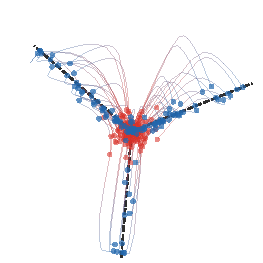
\includegraphics[width=.34\linewidth]{figures/gradflow-mlp-homogeneous-relu/neuron-trajectories.pdf} &
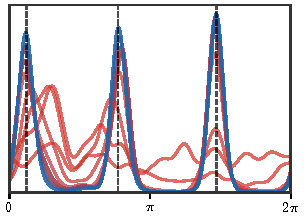
\includegraphics[width=.34\linewidth]{figures/gradflow-mlp-homogeneous-relu/direction-histogram.pdf}
\end{tabular}
\caption{\emph{Mean-field training of a homogeneous two-layer model as transport in neuron space.} The left panel shows the Wasserstein particle gradient flow in the reduced homogeneous coordinates $(|u|v_1,|u|v_2)$, with black dashed rays marking the teacher directions. The right panel shows the weighted angular density along a front-loaded sequence of times, colored from red to blue, so that the early concentration of neuron directions is visible.}
\index{two-layer neural network}% strictindex
\index{gradient!flow}% strictindex
\label{fig:gradflow-mlp-homogeneous-relu}
\end{figure}

\paragraph{Classical convexity and stationarity.}
\index{convexity!classical}% strictindex
\index{stationarity}% strictindex
Before using the specific homogeneity mechanism of Chizat and Bach, it is useful to isolate a simpler convex-analytic principle behind many mean-field arguments. Consider an energy of the form
\[
	f(\alpha)
	=
	\frac12\iint k(x,x')\d\alpha(x)\d\alpha(x')
	+
	\int V(x)\d\alpha(x)
	+C,
\]
on probability measures over a parameter domain. Assume that the quadratic part is convex in the classical sense, namely convex for the affine structure of measures:
\index{probability measure}% strictindex
\[
	Q((1-s)\alpha+s\beta)\leq (1-s)Q(\alpha)+sQ(\beta),
	\qquad
	Q(\alpha)=\frac12\iint k\d\alpha\d\alpha.
\]
This is ordinary convexity of the functional on the convex set of measures, not displacement convexity along $\Wass_2$ geodesics.
\index{convexity!along geodesics}% strictindex
\index{displacement convexity}% strictindex

\begin{prop}[Affine convexity and stationary positive densities]\label{prop-classical-convex-stationary}
\index{convexity!classical}% strictindex
\index{stationary density}% strictindex
		Let $\Omega\subset\RR^d$ be connected and open, let $f=Q+\int V\,\d\alpha+C$ be as above on $\Pp_2(\Omega)$, and assume that $Q$ is classically convex. Suppose that $\alpha_t\in AC^2_{\mathrm{loc}}([0,+\infty);\Pp_2(\Omega))$ is an energy-dissipation solution of the Wasserstein gradient flow of $f$, with $f(\alpha_0)<+\infty$, and converges in $\Wass_2$ to $\alpha_\infty=\rho_\infty\d x$, where $\rho_\infty>0$ almost everywhere on $\Omega$, and that $\inf_{t\geq0}f(\alpha_t)>-\infty$. Assume that $\delta f(\alpha_\infty)\in C^1(\Omega)$, that the first-variation formula and the affine subgradient inequality hold along every finite-energy segment from $\alpha_\infty$, that $f(\alpha_\infty)<+\infty$, and that the squared Wasserstein slope is lower semicontinuous along the convergence, in the sense that
\index{stationary condition}% strictindex
\index{first variation}% strictindex
\index{stationarity}% strictindex
\index{Wasserstein!gradient}% strictindex
\index{gradient!flow}% strictindex
\index{Wasserstein!gradient flow}% strictindex
	\[
		\int_\Omega\norm{\nabla\delta f(\alpha_\infty)}^2\d\alpha_\infty
		\leq
		\liminf_{n\to\infty}
		\int_\Omega\norm{\nabla\delta f(\alpha_{t_n})}^2\d\alpha_{t_n}
	\]
	whenever $t_n\to\infty$. Then $\alpha_\infty$ is a global minimizer of $f$.
\index{global!minimizer}% strictindex
\end{prop}
\begin{proof}
	The energy-dissipation inequality and the lower bound on $f$ along the convergent trajectory imply
	\[
		\int_0^\infty
		\int_\Omega\norm{\nabla\delta f(\alpha_t)}^2\d\alpha_t\d t
		<+\infty.
	\]
	Hence there exists $t_n\to\infty$ for which the inner integral tends to zero. The assumed lower semicontinuity gives
\index{gradient!flow}% strictindex
	\[
		\int_\Omega \norm{\nabla \delta f(\alpha_\infty)}^2\d\alpha_\infty=0.
	\]
	Because $\rho_\infty>0$ almost everywhere and $\nabla\delta f(\alpha_\infty)$ is continuous, this gradient vanishes throughout $\Omega$. Connectedness then implies that $\delta f(\alpha_\infty)$ is constant. Consequently, for every $\beta\in\Pp_2(\Omega)$ with $f(\beta)<+\infty$,
	\[
		\int_\Omega\delta f(\alpha_\infty)\d(\beta-\alpha_\infty)=0.
	\]
	Classical convexity of $f$ in the affine variable $\alpha$ gives the subgradient inequality
\index{subgradient inequality}% strictindex
\index{first variation}% strictindex
\index{convexity!classical}% strictindex
	\[
		f(\beta)\geq f(\alpha_\infty)
		+
		\int \delta f(\alpha_\infty)\d(\beta-\alpha_\infty)
		= f(\alpha_\infty).
	\]
	The same conclusion is immediate when $f(\beta)=+\infty$, so no competitor in $\Pp_2(\Omega)$ has smaller energy. Strict positivity is essential to this argument: without it, stationarity controls the first variation only on the support explored by the limiting measure. For square-loss two-layer mean-field models, \eqref{eq-mlp-square-loss-quadratic-linear} is exactly of this quadratic-plus-linear form, and positive semidefiniteness of the induced kernel $k$ is the classical convexity assumption.
\index{linear!form}% strictindex
\index{two-layer neural network}% strictindex
\index{convexity!classical}% strictindex
\end{proof}

The convergence theory then separates two regimes. Chizat and Bach show that, under their regularity, homogeneity, support-propagation and Sard-type assumptions, any $\Wass_2$-convergent unregularized noiseless flow has a globally minimizing limit~\citep{ChizatBach2018OverparameterizedOT}; this conditional result does not assert convergence of every trajectory. Mei, Montanari and Nguyen prove convergence for noisy, regularized dynamics under their stated regularity and initialization assumptions~\citep{MeiMontanariNguyen2018MeanFieldNN}: at the PDE level nondegenerate noise adds diffusion and smooths the law for positive time. Rotskoff and Vanden-Eijnden emphasize the parameters-as-particles interpretation, long-time convergence and asymptotic error scaling with the network width under their model assumptions~\citep{RotskoffVandenEijnden2018Trainability}. The following formal statement isolates the noiseless Chizat--Bach mechanism and ignores the technical issues due to ReLU non-smoothness, support propagation and compactness.
\index{noisy gradient descent}% strictindex
\index{interacting particle system}% strictindex

\begin{prop}[Formal global optimality for two-homogeneous mean-field flows]\label{prop-formal-chizat-bach}
\index{global!optimality}% strictindex
	Assume that the feature is positively two-homogeneous in the neuron variable,
\index{neuron}% strictindex
	\[
		\psi(\lambda x,z)=\lambda^2\psi(x,z)
		\qquad(\lambda>0),
	\]
	and that $f(\alpha)=J(G_\alpha)$ with $J$ convex and differentiable as a functional of the predictor. Let $\alpha$ be a smooth stationary point of the Wasserstein flow, so that $\nabla_x\delta f(\alpha)(x)=0$ on $\supp(\alpha)$. Assume also full directional support: for every unit direction $\omega$, the support of $\alpha$ intersects the ray $\{\lambda\omega:\lambda>0\}$. Then $\alpha$ is a global minimizer of $f$ over the mean-field model class.
\index{stationarity}% strictindex
\index{global!minimizer}% strictindex
\end{prop}
\begin{proof}
	Choose the first-variation representative
	\[
		h_\alpha(x)=\delta f(\alpha)(x)
		=
		DJ(G_\alpha)\bigl[\psi(x,\cdot)\bigr].
	\]
	When the predictor space is $L^2(\zeta)$ and $DJ(G_\alpha)$ has a Riesz representative, this derivative-dual pairing can equivalently be written as the $L^2(\zeta)$ inner product with that representative. The abstract notation above is all that is needed here.
	Additive constants in first variations do not affect the Wasserstein gradient or first-order inequalities between probability measures; this normalization is useful because it inherits the homogeneity of $\psi$. By two-homogeneity of $\psi$, one has
	\[
		h_\alpha(\lambda x)=\lambda^2h_\alpha(x),
		\qquad \lambda>0.
	\]
	Taking \(x=0\) and any \(\lambda\neq1\) in this identity gives \(h_\alpha(0)=0\). We first record that stationarity forces \(h_\alpha\) to vanish on \(\supp(\alpha)\). Indeed, if \(x=r\omega\in\supp(\alpha)\) with \(r>0\) and \(\norm{\omega}=1\), then
	\[
		0=\dotp{\nabla h_\alpha(r\omega)}{\omega}
		=\frac{\d}{\d s}h_\alpha(s\omega)\bigg|_{s=r}
		=2r h_\alpha(\omega),
	\]
	so \(h_\alpha(\omega)=0\), and hence \(h_\alpha(x)=r^2h_\alpha(\omega)=0\). The case \(x=0\) has already been covered, so \(h_\alpha=0\) on \(\supp(\alpha)\) and \(\int h_\alpha\,\d\alpha=0\).

	We now argue by contradiction. Suppose that a competitor \(\beta\) satisfies \(f(\beta)<f(\alpha)\). Since
	\[
		G_\beta-G_\alpha
		=
		\int \psi(x,\cdot)\d(\beta-\alpha)(x),
	\]
	convexity of \(J\) gives
	\[
		f(\beta)-f(\alpha)
		\geq
		\int h_\alpha(x)\d(\beta-\alpha)(x).
	\]
	The left-hand side is negative, while \(\int h_\alpha\,\d\alpha=0\), so \(\int h_\alpha\,\d\beta<0\). Since \(h_\alpha(0)=0\), this strict negativity must occur away from the origin: there exists a nonzero point \(x=r\omega\) with \(r>0\), \(\norm{\omega}=1\), and \(h_\alpha(x)<0\). Equivalently \(h_\alpha(\omega)=h_\alpha(x)/r^2<0\). By full directional support, there is \(r_\omega>0\) such that \(r_\omega\omega\in\supp(\alpha)\). At this support point,
	\[
		\dotp{\nabla h_\alpha(r_\omega\omega)}{\omega}
		=
		2r_\omega h_\alpha(\omega)
		<0,
	\]
	which contradicts the stationarity condition \(\nabla h_\alpha=0\) on \(\supp(\alpha)\). Thus no competitor has smaller risk.

	The rigorous Chizat--Bach theorem replaces the full directional support assumption by propagation and overparameterization hypotheses ensuring that any negative first-variation direction is represented by the evolving support. The same radial-derivative contradiction, applied after this support-propagation step, then rules out non-optimal stationary limits.
\index{stationarity}% strictindex
\end{proof}

\paragraph{Other geometries of descent.}\label{par-generalized-flow-perspectives}
Changing the transport action changes the steepest-descent dynamics, as suggested by the extensions at the end of Section~\ref{sec-benamou-brenier-dynamic}. Nonlinear mobilities lead to diffusion laws adapted to density-dependent transport~\citep{dolbeault2009new}; graph and jump geometries realize reversible Markov evolution or suitable nonlocal diffusions as entropy gradient flows~\citep{Maas2011,Erbar2012JumpEntropy}. Allowing mass to change adds a reaction mechanism to transport and connects to particle reweighting and birth--death algorithms~\citep{gallouet2017jko,Chizat2021GradientMethodsMeasures,Rotskoff2019BirthDeath}. Such choices require their own well-posedness and convergence theory. The next subsection develops the particular extension needed for deep-network training: a family of ordinary Wasserstein flows indexed by depth.

\subsection{Conditional Wasserstein Training of Infinite ResNets}
\index{conditional!Wasserstein flow}% strictindex
\index{ResNet!infinite-depth}% strictindex
\label{sec-conditional-wasserstein-resnets}
\index{conditional!optimal transport}% strictindex
\index{conditional!Wasserstein distance}% strictindex
\index{ResNet}% strictindex
Residual networks learn small residual updates around the identity~\citep{HeZhangRenSun2016ResNet}. This makes depth behave like time: very deep residual architectures can be interpreted as discretizations of differential equations, a viewpoint developed in stable architectures, neural ODEs and mean-field optimal-control models of deep learning~\citep{HaberRuthotto2017StableArchitectures,LuZhongLiDong2018BeyondFiniteLayers,Chen2018NeuralODE,EHanLi2019MeanFieldDeepLearning}. The conditional-OT formulation of Barboni, Peyr\'e and Vialard~\citep{BarboniPeyreVialard2024ConditionalResNets} studies the width mean-field limit for an already continuous-depth model. Passage from a finite-depth ResNet to that neural ODE is a separate approximation problem, not part of the same theorem. This should be read alongside the broader conditional-transport literature, especially fibered gradient flows~\citep{PeszekPoyato2023FiberedOptimalTransport}, function-space conditional OT~\citep{HosseiniHsuTaghvaei2023ConditionalFunctionSpaces}, and conditional OT flow-matching constructions~\citep{ChemseddineHagemannSteidlWald2024ConditionalWasserstein,KerriganMiglioriniSmyth2024DynamicConditionalOT}. Its conditional Wasserstein distance integrates the quadratic transport geometry of Section~\ref{sec-benamou-brenier-dynamic} over the fixed depth variable. The point of the construction is to keep track of two independent symmetries: neurons can be relabelled inside each layer, but mass should not move from one depth to another. Conditional Wasserstein geometry implements exactly this rule. It transports neurons fiber by fiber in parameter space, while the depth variable remains fixed.

We distinguish three levels of description: a finite labelled ResNet, a measure-valued model at fixed depth, and the continuous-depth conditional model. The two transitions should not be conflated. A joint width--depth limit requires an order of limits and estimates uniform in the other discretization parameter; below the finite models motivate the geometry, while the cited rigorous width result concerns the continuous-depth level.

\paragraph{Finite-depth finite-width ResNets.}
\index{ResNet!finite-depth}% strictindex
\index{ResNet!finite-width}% strictindex
\index{residual block}% strictindex
The starting point is the ordinary architecture: depth is discrete, width is finite, and each layer carries a labelled collection of neurons. Fix a parameter space $\Theta\subset\RR^q$, a residual feature $\psi:\Theta\times\RR^d\to\RR^d$, a data law $\zeta$ on input-label pairs $(z,y)$, and a loss $\ell$. With $L$ layers, step size $\tau=1/L$, widths $n_r$, and parameters $\theta_{r,i}\in\Theta$, a finite ResNet is the composition of the residual updates
\begin{equation}\label{eq-finite-resnet}
	z_{r+1}
	=
	z_r+\tau G_{r,n_r}(z_r),
	\qquad
	G_{r,n_r}(z)
	\eqdef
	\frac1{n_r}\sum_{i=1}^{n_r}\psi(\theta_{r,i},z),
	\qquad
	z_0=z,\qquad r=0,\ldots,L-1.
\end{equation}
The associated population loss, with $n=(n_0,\ldots,n_{L-1})$, is
\[
	f_{L,n}((\theta_{r,i})_{r,i})
	=
	\int \ell(z_L^{\theta}(z),y)\d\zeta(z,y).
\]
Equivalently, each layer carries an empirical neuron law
\[
	\alpha_r
	=
	\frac1{n_r}\sum_{i=1}^{n_r}\delta_{\theta_{r,i}},
	\qquad
	G_{r,n_r}(z)
	=
	\int_\Theta\psi(\theta,z)\d\alpha_r(\theta).
\]
Thus a finite ResNet is already a discrete conditional measure on depth and neuron space,
\[
	\alpha^{L,n}(\d s,\d\theta)
	=
	\frac1L\sum_{r=0}^{L-1}\delta_{s_r}(\d s)\alpha_r(\d\theta),
	\qquad
	s_r=r/L,
\]
whose marginal on the depth variable is the discrete measure $\lambda_L=L^{-1}\sum_{r=0}^{L-1}\delta_{s_r}$.
\index{empirical!measure}% strictindex
\index{neuron}% strictindex

\paragraph{Finite-depth mean-field limit.}
\index{ResNet!finite-depth mean-field}% strictindex
At fixed depth, the natural mean-field description removes neuron labels inside each layer. Each empirical law $\alpha_r$ is replaced by a probability measure in $\Pp_2(\Theta)$, and each residual block becomes a mean-field residual block
\[
	z_{r+1}
	=
	z_r+\tau G_{\alpha_r}(z_r),
	\qquad z_0=z,
	\qquad
	G_{\alpha_r}(z)
	\eqdef
	\int_\Theta\psi(\theta,z)\d\alpha_r(\theta).
\]
The loss becomes a functional of the finite family of layer measures,
\[
	f_L(\alpha_0,\ldots,\alpha_{L-1})
	=
	\int \ell(z_L^\alpha(z),y)\d\zeta(z,y).
\]
This motivates the conditional metric defined next, with discrete condition marginal $\lambda_L$: each fiber $s_r$ carries a Wasserstein geometry on neuron laws.

\paragraph{Continuous-depth conditional geometry.}
\index{ResNet!continuous-depth}% strictindex
\index{depth variable}% strictindex
\index{conditional!neuron law}% strictindex
The continuous-depth model turns the layer index into a conditioning variable. It is no longer described by one neuron law, nor even by a finite list of them, but by a family of neuron laws indexed by depth. The state is therefore a conditional probability law
\[
	\alpha(\d s,\d\theta)=\alpha_s(\d\theta)\d s,
\]
or, equivalently, a probability measure on $[0,1]\times\Theta$ whose first marginal is Lebesgue measure. The conditional Wasserstein metric compares the conditional laws at each fixed condition and integrates their squared transport distances. Here the condition is continuous depth, $s\in[0,1]$, the condition law is $\lambda(\d s)=\d s$, and the fiber space is the neuron parameter space $\Theta$. For two conditional neuron laws $\alpha(\d s,\d\theta)=\alpha_s(\d\theta)\d s$ and $\beta(\d s,\d\theta)=\beta_s(\d\theta)\d s$, assume $\int_0^1\int_\Theta\norm{\theta}^2\d\alpha_s(\theta)\d s<+\infty$ and likewise for $\beta$. The relevant distance is the depthwise quadratic Wasserstein metric
\begin{equation}\label{eq-resnet-depth-wasserstein}
	\Wass_{2,\lambda}^2(\alpha,\beta)
	=
	\int_0^1\Wass_2^2(\alpha_s,\beta_s)\d s.
\end{equation}
It compares neurons only at the same depth: transport in $\theta$ is allowed fiber by fiber, while mass is not transported between layers.

\paragraph{Infinite-depth mean-field ResNet.}
\index{ResNet!infinite-depth}% strictindex
Once depth is continuous, the forward pass is a controlled ODE and the control is the conditional neuron law. A mean-field infinite-depth and infinite-width ResNet is described by a measurable family $s\mapsto\alpha_s\in\Pp_2(\Theta)$. Each slice is the neuron law of one infinitesimal residual block, and the feature $\psi(\theta,z)$ now acts as a vector field on the state variable. The forward pass is
\begin{equation}\label{eq-mean-field-resnet-forward}
	\partial_s z_s
	=
	G_{\alpha_s}(z_s)
	\eqdef
	\int_\Theta \psi(\theta,z_s)\d\alpha_s(\theta),
	\qquad z_0=z.
\end{equation}
The population risk is
\[
	f_{\mathrm{Res}}(\alpha)
	=
	\int \ell(z_1^\alpha(z),y)\d\zeta(z,y).
\]
Under the usual regularity assumptions ensuring well-posedness of the ODE, this defines a functional on the conditional Wasserstein space.

\paragraph{Conditional Wasserstein gradient flow.}
\index{layerwise matching}% strictindex
\index{conditional!gradient flow}% strictindex
Training is now steepest descent for an objective on conditional laws. More generally, let $(S,\lambda)$ be a probability space of conditions and let $f$ be a differentiable functional on measures $\alpha(\d s,\d\theta)=\alpha_s(\d\theta)\lambda(\d s)$ with fixed first marginal $\lambda$. For signed perturbations $\xi(\d s,\d\theta)=\xi_s(\d\theta)\lambda(\d s)$ satisfying $\int_\Theta\d\xi_s=0$ for $\lambda$-a.e.\ $s$, we use the fiberwise first-variation convention
\[
	\frac{\d}{\d\varepsilon}f(\alpha+\varepsilon\xi)\bigg|_{\varepsilon=0}
	=
	\int_S\int_\Theta \frac{\delta f}{\delta\alpha_s}(\alpha)(\theta)\d\xi_s(\theta)\d\lambda(s).
\]
The formal conditional Wasserstein gradient flow is the family of continuity equations
\begin{equation}\label{eq-conditional-resnet-gradient-flow}
	\partial_t\alpha_{t,s}
	+\diverg_\theta(\alpha_{t,s}v_{t,s})=0,
	\qquad
	v_{t,s}(\theta)
	=
		-\nabla_\theta\frac{\delta f}{\delta\alpha_s}(\alpha_t)(\theta),
\end{equation}
for $\lambda$-a.e.\ condition $s$, whenever the first variation is differentiable in the parameter variable. In the ResNet case one takes $f=f_{\mathrm{Res}}$ and $S=[0,1]$. The equation is fiberwise in its transport geometry, but not decoupled as a training dynamics: changing $\alpha_s$ affects the terminal loss through the forward ODE and the corresponding adjoint equation. Thus each depth performs a Wasserstein steepest descent in its own neuron space, while all depths interact through the state trajectory.
\index{first variation}% strictindex
\index{Wasserstein!gradient flow}% strictindex

\paragraph{Particle discretization and layerwise matching.}
\index{ResNet!particle discretization}% strictindex
The finite network is recovered by discretizing both the condition variable and the fiber measures. With the discrete depth marginal $\lambda_L$, finite-depth finite-width ResNets are particle approximations of the conditional flow above. If two networks have the same depth grid and the same widths, and if their empirical layer laws are
\[
	\alpha_r=\frac1{n_r}\sum_{i=1}^{n_r}\delta_{\theta_{r,i}},
	\qquad
	\beta_r=\frac1{n_r}\sum_{i=1}^{n_r}\delta_{\theta'_{r,i}},
\]
then their squared conditional distance is
\[
	\Wass_{2,\lambda_L}^2(\alpha^{L,n},\beta^{L,n})
	=
	\frac1L\sum_{r=0}^{L-1} \Wass_2^2(\alpha_r,\beta_r).
\]
Keeping neuron labels fixed gives the labelled parameter distance
\[
	\frac1L\sum_{r=0}^{L-1}\frac1{n_r}
	\sum_{i=1}^{n_r}\norm{\theta_{r,i}-\theta'_{r,i}}^2,
\]
which corresponds to a particular feasible coupling and therefore upper bounds the squared conditional Wasserstein distance. The Riemannian metric represented by this normalization is
\[
	\norm{\dot\theta}^2
	=
	\frac1L\sum_{r=0}^{L-1}\frac1{n_r}
	\sum_{i=1}^{n_r}\norm{\dot\theta_{r,i}}^2.
\]
Consequently, its coordinate gradient flow is \(\dot\theta_{r,i}=-Ln_r\nabla_{\theta_{r,i}}f_{L,n}\); an implementation using ordinary coordinate gradients must absorb this factor into the layerwise learning rate. Optimizing over permutations inside each equal-weight layer gives the Wasserstein matching term above. Under the regularity and compact-support assumptions of~\citet{BarboniPeyreVialard2024ConditionalResNets}, finite-width particle training converges to the continuous-depth conditional flow. Consistency of a finite-depth discretization, and especially a simultaneous width--depth limit, is a separate question requiring an explicit order of limits and uniform estimates. In this sense, the shallow mean-field flow is the one-fiber case, whereas infinitely deep ResNets require a continuum of Wasserstein flows indexed by depth and coupled through the network state.
\index{continuous!depth}% strictindex
\index{residual network}% strictindex
\index{mean-field neural network}% strictindex
\index{Wasserstein!gradient flow}% strictindex

The progression from particles to shallow and deep networks keeps the same principle: the energy specifies what training decreases, while the transport geometry specifies how the parameter law can move. Geodesic convexity and slope inequalities provide convergence guarantees in the cases where they hold. We now turn to generative models, whose prescribed or learned velocities need not come from such a variational structure.

\FloatBarrier

% !TEX root = ../PDE4ML.tex

\section{Generative Models via Transportation}
\index{generative model}% strictindex
\label{sec-generative-models-transportation}

The Wasserstein gradient-flow calculus developed in Section~\ref{sec-wasserstein-gradient-flows} is variational. Modern machine-learning models often use the same transportation language more broadly: one may prescribe an interpolation and regress its velocity, fit a one-step generator to a descent field, or view network depth as a continuous transport of token measures. The examples below separate what is genuinely a Wasserstein gradient flow from what is a transportation dynamics with a useful geometric interpretation.
\index{Wasserstein!gradient}% strictindex
\index{gradient!flow}% strictindex
\index{Wasserstein!gradient flow}% strictindex
\index{token measure}% strictindex
\index{one-step generative model}% strictindex

\subsection{Generative Models via Flow Matching}
\label{sec-generative-flow-matching}
\index{flow matching}% strictindex
\index{generative model}% strictindex

Flow matching constructs a generative map by learning an Eulerian velocity field for a prescribed interpolation. The key computational insight is that an unconstrained regression produces one field satisfying the continuity equation. It need not be the minimum-kinetic-energy Wasserstein tangent of that same measure curve.
\index{velocity field}% strictindex
\index{continuity equation}% strictindex

Generative models aim to build a transportation map $T$ between a reference distribution $\alpha$ (typically an isotropic Gaussian) and the target data distribution $\beta$. Since such reference measures are non-atomic, a measurable map with $T_\sharp\alpha=\beta$ exists on standard Borel spaces, for instance by identifying the atomless source probability space with a uniform variable on the unit interval and realizing the target as a measurable image of that variable. The target itself need not be atomless. This abstract existence statement is much weaker than having an explicit and numerically stable construction of $T$.
\index{reference!distribution}% strictindex
\index{reference!measure}% strictindex
\index{generative model}% strictindex
%
Optimal transport is one approach to achieving this, but it is computationally expensive and raises questions about how to estimate it from samples. A different route is to prescribe an interpolation between noise and data, learn its velocity, and obtain $T$ by integrating a time-dependent vector field $v_t$. This point of view sits at the meeting point of two literatures, surveyed from a transport perspective in~\citet{Peyre2026OptimalDiffusionTransports}. The diffusion branch builds on score matching~\citep{Hyvarinen2005ScoreMatching}, denoising score matching~\citep{Vincent2011DenoisingScoreMatching}, nonequilibrium noising chains~\citep{SohlDickstein2015DeepUnsupervised}, denoising diffusion probabilistic models~\citep{Ho2020DDPM}, score-based generative modeling~\citep{Song2019ScoreMatchingGenerative}, and the continuous-time score-SDE/probability-flow formulation~\citep{Song2021ScoreSDE}. The deterministic regression branch was introduced, essentially in parallel, under three closely related names: flow matching~\citep{Lipman2022FlowMatching}, rectified flow~\citep{Liu2023RectifiedFlow}, and stochastic interpolants~\citep{Albergo2025StochasticInterpolants}. In all three cases, the computational object is a velocity field whose regression loss avoids simulating the learned ODE during training.
\index{stochastic!interpolant}% strictindex
\index{diffusion model}% strictindex
\index{score-SDE}% strictindex
\index{flow!probability ODE}% strictindex
\index{score-based generative modeling}% strictindex
\index{velocity field}% strictindex
\index{flow matching}% strictindex
\index{time-dependent vector field}% strictindex
\index{denoising score matching}% strictindex
\index{stochastic!interpolant}% strictindex
\index{regression loss}% strictindex
\index{flow!rectified}% strictindex
%
After constructing an interpolation $\alpha_t$, the weighted-Poisson problem~\eqref{eq:least-square-field-explicit}, whenever its finite-action assumptions hold, selects its minimum-\(L^2(\alpha_t)\)-norm tangent in the closure of gradient fields. A parametric push-forward provides another admissible field directly: the conditional expectation of the latent path velocities. It is learned by an unconstrained least-squares regression and therefore avoids a Poisson solve. The two representatives differ in general by a field \(w_t\) satisfying \(\diverg(\alpha_t w_t)=0\); they coincide when the conditional-expectation field is itself a tangent gradient. For the Gaussian product interpolation below, this holds when the endpoint covariances commute, but need not hold otherwise.
\index{conditional!expectation}% strictindex
\index{push-forward}% strictindex

\paragraph{Deterministic interpolants.}
\index{deterministic interpolant}% strictindex
\index{temporal noise}% strictindex
\index{stochastic!interpolant}% strictindex

A deterministic interpolant first couples the two endpoint laws and then assigns an absolutely continuous path to almost every paired sample. Once the pair is fixed, the path carries no additional temporal randomness. This construction separates the choice of endpoint correspondence from the geometry of the paths joining corresponding points.
\begin{defn}[Deterministic interpolant]\label{def-deterministic-interpolant}
Let \(\pi\in\Couplings(\alpha_0,\alpha_1)\). A deterministic interpolant is a jointly measurable family \(I_t:\RR^d\times\RR^d\to\RR^d\) such that \(t\mapsto I_t(x,y)\) is absolutely continuous for \(\pi\)-almost every \((x,y)\), its derivative is jointly measurable, \(\int_0^1\!\int_{\RR^d\times\RR^d}\norm{\partial_t I_t(x,y)}\,\d\pi(x,y)\d t<+\infty\), and \(I_0(x,y)=x\), \(I_1(x,y)=y\) for \(\pi\)-almost every \((x,y)\).
It induces \(\alpha_t=(I_t)_\sharp\pi\) and has pathwise velocity \(\partial_t I_t(x,y)\).
\end{defn}
More generally, $\alpha_t$ can be obtained by pushing a latent distribution $\pi \in \Pp(\RR^{d'})$ through a time-dependent map $I_t : \RR^{d'} \to \RR^d$; the latent dimension $d'$ may be larger than the data dimension $d$, i.e.
\begin{equation}\label{eq:interp-coupling}
	\forall t \in [0,1], \quad \alpha_t := (I_t)_\sharp \pi.
\end{equation}
The basic two-endpoint construction already covers most flow-matching paths used in practice.

\begin{example}[Linear two-endpoint deterministic interpolants]
	Set $d'=2d$, write $(x,y)\in\RR^d\times\RR^d$, and choose the straight path $I_t(x,y)=(1-t)x+ty$. If $\pi$ has marginals $(\alpha_0,\alpha_1)$, then $\alpha_t=(I_t)_\sharp\pi$ interpolates between the two endpoint laws.
	With this linear path and an arbitrary coupling $\pi$, the regression below is the common core of flow matching and rectified flow: Lipman et al.\ emphasize conditional probability paths and simulation-free training of continuous normalizing flows, while rectified flow emphasizes straight couplings, reflow, and the possibility of reducing transport costs and discretization error~\citep{Lipman2022FlowMatching,Liu2023RectifiedFlow}.
\index{flow!rectified}% strictindex
\index{flow matching}% strictindex

	More complex constructions are possible when sampling from $\pi$ remains simple. Static auxiliary randomness is still handled by enlarging the latent variable, while Brownian noise leads to the diffusion correction described below; this is the broader stochastic-interpolant viewpoint connecting deterministic flows, probability-flow ODEs and diffusion SDEs~\citep{Albergo2025StochasticInterpolants}.
\index{flow!probability ODE}% strictindex
\end{example}
\index{flow!continuous normalizing}% strictindex
\index{reflow}% strictindex
\index{discretization error}% strictindex
\index{latent!variable}% strictindex
\index{conditional!probability}% strictindex
\index{flow!normalizing}% strictindex
\index{probability path}% strictindex
\index{flow matching}% strictindex
\index{flow!rectified}% strictindex
\index{flow!probability ODE}% strictindex
\index{trivial coupling}% strictindex

\begin{rem}[Independent and optimal-transport couplings]
The two most common constructions use either independent endpoint samples or an optimal-transport coupling. For $\pi=\alpha_0\otimes\alpha_1$, if $\alpha_0=n^{-1}\sum_i\delta_{x_i}$ and $\alpha_1=m^{-1}\sum_j\delta_{y_j}$, then $\alpha_t=(nm)^{-1}\sum_{i,j}\delta_{I_t(x_i,y_j)}$ is represented by $nm$ labelled particles, possibly at coincident locations. At the opposite geometric extreme, if $T$ is the quadratic-optimal Brenier map from $\alpha_0$ to $\alpha_1$, the coupling $\pi=(\Id,T)_\sharp\alpha_0$ with the straight interpolant gives $\alpha_t=((1-t)\Id+tT)_\sharp\alpha_0$, namely the McCann displacement interpolation. Figure~\ref{fig:generative-flow-matching-interpolants} separates these two choices of endpoint coupling from the separate choice of path joining each pair.
\index{Dirac mass}% strictindex
\end{rem}

\begin{figure}[htbp]
\centering
\begin{tabular}{@{}ccc@{}}
\small product pairing & \small OT pairing & \small curved bridge \\[-.15em]
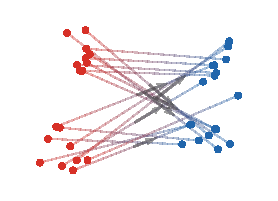
\includegraphics[width=.30\linewidth]{figures/generative-flow-matching-interpolants/product-linear.pdf} &
\index{flow matching}% strictindex
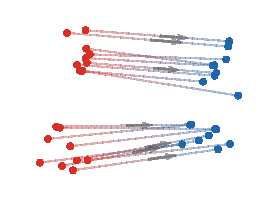
\includegraphics[width=.30\linewidth]{figures/generative-flow-matching-interpolants/ot-linear.pdf} &
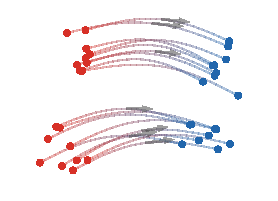
\includegraphics[width=.30\linewidth]{figures/generative-flow-matching-interpolants/curved-bridge.pdf}
\end{tabular}
\caption{\emph{Flow matching interpolants between the same empirical source and target measures.} A product-style random pairing produces crossing paths, an OT pairing gives direct displacement rays, and a curved bridge changes the path geometry while keeping the same endpoints. Gray arrows mark representative midpoint velocities $\partial_t I_t$.}
\label{fig:generative-flow-matching-interpolants}
\end{figure}

\paragraph{Learning a flow field.}
\index{flow matching}% strictindex

This interpolation is not directly useful for sampling from $\beta$, but it can be used to define a flow field $v_t$ so that the Eulerian advection equation~\eqref{eq:eulerian-advection} holds.
%
This flow field is computed by solving an unconstrained least-squares problem, or equivalently, it is a conditional expectation.
\index{conditional!expectation}% strictindex

\begin{prop}[Flow matching vector field]\label{prop-flow-matching-vector-field}
	Assume that $t\mapsto I_t(u)$ is absolutely continuous for $\pi$-almost every $u$, that its derivative $(t,u)\mapsto\partial_t I_t(u)$ is jointly measurable, and that \(\int_0^1\!\int_{\RR^{d'}}\norm{\partial_t I_t(u)}^2\d\pi(u)\d t<+\infty\).
	Let \(U\sim\pi\) and \(X_t=I_t(U)\), so that \(X_t\sim\alpha_t\).
	For almost every $t$, consider the flow-matching problem over \(v_t\in L^2(\alpha_t;\RR^d)\)
\index{flow matching}% strictindex
	\begin{equation}
		\min_{v_t} \int_{\RR^{d'}} \norm{v_t(I_t(u)) - [\partial_t I_t](u)}^2 \, \d\pi(u). \label{eq:flow-matching}
	\end{equation}
	Its minimizer is characterized $\alpha_t$-almost everywhere by
\index{conditional!expectation}% strictindex
	\begin{equation}\label{eq:flow-match-conditional}
		v_t(x)=\EE\bigl[\partial_t I_t(U)\mid X_t=x\bigr].
	\end{equation}
	There is a jointly measurable choice \((t,x)\mapsto v_t(x)\), obtained by disintegrating \(\d t\,\pi(\d u)\) under \((t,u)\mapsto(t,I_t(u))\). For this choice, $v_t\in L^2(\alpha_t;\RR^d)$ for almost every $t$, and the pair $(\alpha_t,v_t)$ satisfies the continuity equation~\eqref{eq:eulerian-advection} in the distributional sense on $(0,1)\times\RR^d$.
\index{continuity equation}% strictindex
\end{prop}

\begin{proof}
	The push-forward identity reads \(\int_{\RR^d}\varphi(x)\,\d\alpha_t(x)=\int_{\RR^{d'}}\varphi(I_t(u))\,\d\pi(u)\) for every bounded continuous test function $\varphi$.
\index{push-forward}% strictindex
	For almost every $t$, the minimizer in~\eqref{eq:flow-matching} is the orthogonal projection in $L^2(\pi;\RR^d)$ of the latent velocity $\partial_t I_t(u)$ onto the closed subspace of functions that depend on $u$ only through $I_t(u)$. This projection is the conditional expectation~\eqref{eq:flow-match-conditional}. Equivalently, disintegration of the joint measure \(\d t\,\pi(\d u)\) by the map \((t,u)\mapsto(t,I_t(u))\) supplies a jointly measurable version. Conditional Jensen gives \(\int\norm{v_t}^2\d\alpha_t\leq\int\norm{\partial_t I_t}^2\d\pi\),
	so the Eulerian velocity is square-integrable in space--time. Its defining conditional-expectation identity is, for every \(m\in L^2(\alpha_t;\RR^d)\),
\index{conditional!expectation}% strictindex
\index{flow matching}% strictindex
	\begin{equation}\label{eq:v_t}
		\int \dotp{m(x)}{v_t(x)} \, \d\alpha_t(x)
		=
		\int \dotp{m(I_t(u))}{[\partial_t I_t](u)} \, \d\pi(u).
	\end{equation}

	We now prove that this field transports the curve $(\alpha_t)_t$. Testing first with \(\varphi\in C_c^\infty(\RR^d)\), and then integrating against compactly supported smooth functions of time, gives the distributional formulation on space--time. The fixed-time weak identity for
	$\partial_t\alpha_t+\diverg(\alpha_t v_t)=0$ is that, for every $\varphi\in C_c^\infty(\RR^d)$,
	\begin{equation}\label{eq:flow-matching-weak-target}
		\frac{\d}{\d t}\int\varphi(x)\,\d\alpha_t(x)
		-
		\int\dotp{v_t(x)}{\nabla\varphi(x)}\,\d\alpha_t(x)
		=0.
	\end{equation}
	By the pathwise chain rule, $t\mapsto\varphi(I_t(u))$ is absolutely continuous for $\pi$-almost every $u$. The space--time integrability assumption and Fubini's theorem justify integration of its derivative, so the push-forward identity gives, for almost every $t$,
\index{push-forward}% strictindex
\index{flow matching}% strictindex
	\begin{equation}\label{eq:flow-matching-test-derivative}
		\frac{\d}{\d t}\int \varphi(x)\d\alpha_t(x)
		=
		\int \dotp{\nabla\varphi(I_t(u))}{[\partial_t I_t](u)}\d\pi(u).
	\end{equation}
	On the other hand, applying~\eqref{eq:v_t} with $m=\nabla\varphi$ gives
	\begin{equation}\label{eq:flow-matching-velocity-test}
		\int\dotp{v_t(x)}{\nabla\varphi(x)}\,\d\alpha_t(x)
		=
		\int \dotp{\nabla\varphi(I_t(u))}{[\partial_t I_t](u)}\d\pi(u).
	\end{equation}
	Comparing~\eqref{eq:flow-matching-test-derivative} and~\eqref{eq:flow-matching-velocity-test} yields~\eqref{eq:flow-matching-weak-target}, which is the desired continuity equation.
\index{continuity equation}% strictindex
\index{flow matching}% strictindex
\end{proof}

\index{conditional!expectation}% strictindex
\index{disintegration}% strictindex
%
Numerically, $(x,t) \mapsto v_t(x)$ can be parameterized by a neural network, for example a U-Net for image data~\citep{RonnebergerFischerBrox2015UNet}. The least-squares regression~\eqref{eq:flow-matching} can then be optimized over the network parameters using stochastic optimization algorithms.
\index{stochastic!gradient}% strictindex
\index{flow matching}% strictindex
%

\paragraph{Sampling algorithm.}
Once the field $v_t$ has been estimated by the tractable regression~\eqref{eq:flow-matching}, generation amounts to integrating its characteristics. For a sufficiently regular version of the exact population field, let $T_t$ denote the flow map solving
\begin{equation}\label{eq-flow-matching-sampling-map}
	\partial_tT_t(x)=v_t(T_t(x)),
	\qquad T_0(x)=x.
\end{equation}
Assume that this ODE generates a unique measurable flow on every compact subinterval of $[0,1)$ and that the continuity equation is unique in the corresponding solution class. Since the exact field transports the prescribed curve, $(T_t)_\sharp\alpha_0=\alpha_t$ for $t<1$. If the flow map extends to $t=1$, then $(T_1)_\sharp\alpha_0=\alpha_1$; consequently, $X_0\sim\alpha_0$ implies $T_1(X_0)\sim\alpha_1$. Numerically, one draws independent samples from the simple reference law $\alpha_0$ and approximates $T_1$ by solving~\eqref{eq-flow-matching-sampling-map} with the regressed field, so the resulting endpoint law is only approximately $\alpha_1$. For singular endpoints, even the exact flow may instead satisfy only $(T_t)_\sharp\alpha_0=\alpha_t\rightharpoonup\alpha_1$ as $t\uparrow1$, while the velocity or its spatial derivative becomes singular.
\index{transport!map}% strictindex
\index{continuity equation}% strictindex

This inference stage can be expensive because every generated sample requires many neural-field evaluations along an ODE trajectory. Section~\ref{sec-one-step-generative-models} presents the opposite tradeoff: repeated flow estimation or distillation makes training more expensive, but the final sampler is a single network evaluation.

\paragraph{Connection with diffusion models.}\label{par-diffusion-model-connection}
\index{diffusion model}% strictindex

Diffusion models generate data by reversing a progressive noising process. Complementary applied and SDE-based introductions are given by \citet{HighamHighamGrindrod2025DiffusionIntroduction} and \citet{TangZhao2025DiffusionTutorial}. Here we focus on their connection with the interpolants and velocity regression introduced above.

In the special case where $I_t(x,y)=(1-t)x+ty$ is a linear interpolation and $\pi = \alpha_0 \otimes \alpha_1$, the curve $\alpha_t$ is a convolution of rescaled versions of $\alpha_0$ and $\alpha_1$, since convolution is the law of a sum of independent random vectors. The flow-matching problem~\eqref{eq:flow-matching} becomes
\index{flow matching}% strictindex
\[
    \min_{(v_t)_t} \int_0^1\!\int_{\RR^{d} \times \RR^d} \norm{v_t( (1-t)x+t y ) - (y-x) }^2 \, \d\alpha_0(x) \d\alpha_1(y)\,\d t.
\]
When one endpoint is an isotropic Gaussian, this construction is closely related to the probability-flow formulation of diffusion models, up to the usual change of time parametrization~\citep{Song2021ScoreSDE}. This is why flow matching can be viewed both as a deterministic alternative to diffusion training and as a common language for diffusion paths, OT-inspired paths, and rectified paths~\citep{Lipman2022FlowMatching,Liu2023RectifiedFlow,Albergo2025StochasticInterpolants}. The next two propositions are written in the noising direction, from a data law $\alpha$ to a Gaussian; reversing time gives the corresponding sampling flow. They also give an explicit closed form for $v_t$ and show that it is a gradient field.
\index{flow!probability ODE}% strictindex
\index{diffusion model}% strictindex

Figure~\ref{fig:generative-diffusion-2d-forward-backward} illustrates at this point how the scalar coefficients of the interpolant separately control contraction of the data centers and growth of the Gaussian noise.

\begin{figure}[ht]
\centering
\begin{tabular}{@{}c@{}}
\small linear bridge, $a_t=1-t$, $b_t=t$ \\[-.15em]

\includegraphics[width=.72\linewidth]{figures/generative-diffusion-2d-forward-backward/forward-density-linear.pdf} \\[.15em]
\small OU/variance-preserving bridge, $a_t=\cos(\pi t/2)$, $b_t=\sin(\pi t/2)$ \\[-.15em]
\index{bridge!OU}% strictindex
\index{bridge!variance-preserving}% strictindex

\includegraphics[width=.72\linewidth]{figures/generative-diffusion-2d-forward-backward/forward-density-ou.pdf}
\end{tabular}
\caption{\emph{Two-dimensional noising paths from three Dirac masses to a single Gaussian.} The top row shows the linear interpolation $X_t=(1-t)X_0+tZ$, whose component centers move linearly toward the origin and whose covariance grows like $(t\sigma)^2\Id$. The bottom row uses the variance-preserving Ornstein--Uhlenbeck coefficients $a_\tau=e^{-\tau}$ and $b_\tau=\sqrt{1-e^{-2\tau}}$, reparametrized by $\tau=-\log\cos(\pi t/2)$ so that $a_t=\cos(\pi t/2)$ and $b_t=\sin(\pi t/2)$. It has the same endpoints but a different speed of contraction and noising.}
\index{Ornstein-Uhlenbeck@Ornstein--Uhlenbeck!process}% strictindex
\label{fig:generative-diffusion-2d-forward-backward}
\end{figure}
%
For the isotropic Gaussian endpoint considered next, $v_t$ belongs to the tangent-gradient space~\eqref{eq-wasserstein-tangent-space} and is also the minimum-energy velocity of~\eqref{eq:least-square-field}. The regression~\eqref{eq:flow-matching} is computationally simpler because the continuity equation has already been enforced by the chosen interpolant.
\index{continuity equation}% strictindex
%
To prove this, we rely on Tweedie's formula~\citep{Efron2011Tweedie}, which expresses the optimal Gaussian denoiser through the score, i.e.\ the gradient of the log-density.
\index{Gaussian!denoiser}% strictindex
\index{score function}% strictindex
\index{Tweedie identity}% strictindex

\begin{proposition}[Tweedie identity]\label{prop:Tweedie}
Let $W$ be a random vector in $\RR^{d}$ with law $\beta\in\Pp_1(\RR^d)$.
For $\sigma>0$, let $Z\sim\Gaussian(0,\Id)$ be independent of $W$ and observe
\[
Y=W+\sigma Z.
\]
Denote by $\rho_\sigma$ the smooth positive density of \(\beta_\sigma=\beta * \Gaussian(0,\sigma^{2}\Id)\), which is the law of $Y$.
Then the conditional mean admits the following everywhere-defined version:
\[
\EE\bigl[W\mid Y=y\bigr]
      =y+\sigma^{2}\nabla \log \rho_\sigma(y)
\qquad\text{for all } y \in \RR^{d}.
\]
\end{proposition}

\begin{proof}
Let $\varphi_\sigma$ be the $\Gaussian(0,\sigma^{2}\Id)$ density. Bayes' rule gives \(\EE[W\mid Y=y]=\rho_\sigma(y)^{-1}\int_{\RR^{d}} w\varphi_\sigma(y-w)\,\d\beta(w)\).
Differentiating the Gaussian convolution under the integral sign and using
$
\nabla_y\varphi_\sigma(y-w)
     = -\sigma^{-2}(y-w)\,\varphi_\sigma(y-w)
$
yields
\[
\nabla\rho_\sigma(y)
= \int \nabla_y\varphi_\sigma(y-w)\,\d\beta(w)
= -\sigma^{-2}\Bigl(y-\EE[W\mid Y=y]\Bigr)\,\rho_\sigma(y).
\]
Rearranging finishes the proof.
\end{proof}


Tweedie's identity now turns the conditional expectation defining flow matching into an explicit score field for a Gaussian endpoint.

\begin{proposition}[Gaussian-endpoint flow-matching field]\label{prop:flow}
\index{flow matching}% strictindex
Let \(\alpha\in\Pp_2(\RR^d)\), let $X_0\sim\alpha$, and let $Z\sim\Gaussian(0,\Id)$ be independent.
For $t\in(0,1)$ set \(X_t=(1-t)X_0+tZ\) and \(\alpha_t=\operatorname{Law}(X_t)=\rho_t\,\d x\). The minimizer $v^\star:\RR^d\times(0,1)\to\RR^d$ of the flow-matching regression~\eqref{eq:flow-matching} is
\[
v^\star(x,t)
= -\frac{1}{1-t}\,x \;-\; \frac{t}{1-t}\,\nabla\log\rho_t(x)
\qquad (x\in\RR^{d},\;t\in(0,1)).
\]
In particular, for each $t\in(0,1)$ this field is the gradient field \(v^\star(\cdot,t)=-\nabla\bigl(\norm{\cdot}^2/[2(1-t)]+t\log\rho_t/(1-t)\bigr)\).
\end{proposition}

\begin{proof}
Fix $t\in(0,1)$ and write $W=(1-t)X_0$ and $\sigma=t$, so that
$X_t=W+\sigma Z$ matches the setting of Proposition~\ref{prop:Tweedie}.
\index{Tweedie identity}% strictindex
Conditional expectations satisfy
\index{conditional!expectation}% strictindex
$
v^\star(x,t)
= \EE[Z-X_0\mid X_t=x]
= \frac{1}{t}\,\EE[X_t-W\mid X_t=x]
  -\,\frac{1}{1-t}\,\EE[W\mid X_t=x].
$
Applying Proposition~\ref{prop:Tweedie} to $\EE[W\mid X_t=x]$ and
\index{Tweedie identity}% strictindex
noting $\EE[Z\mid X_t=x]=-t\nabla\log\rho_t(x)$
gives the claimed formula.
\end{proof}

Figure~\ref{fig:generative-diffusion-1d-forward-backward} shows both directions of this construction: the prescribed interpolation noising the data and the same probability-flow ODE integrated backward for sampling.

\begin{figure}[ht]
\centering
\begin{tabular}{@{}cc@{}}
\small forward noising & \small reverse probability flow \\[-.15em]
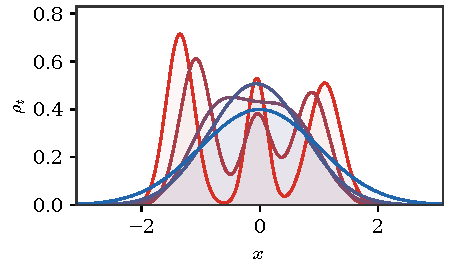
\includegraphics[width=.37\linewidth]{figures/generative-diffusion-1d-forward-backward/forward-densities.pdf} &
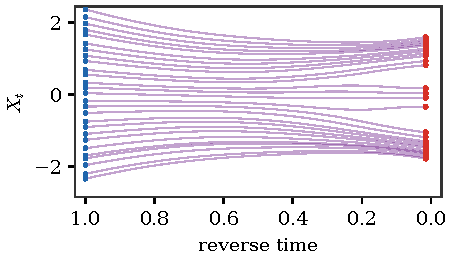
\includegraphics[width=.37\linewidth]{figures/generative-diffusion-1d-forward-backward/backward-trajectories.pdf}
\end{tabular}
\caption{\emph{One-dimensional diffusion bridge for a Gaussian-mixture data law.} The forward path $X_t=(1-t)X_0+tZ$ smooths the red data density toward a blue Gaussian endpoint. Reversing the probability-flow ODE transports stratified, slightly jittered seeds representing that endpoint back toward the data modes, making the splitting of trajectories across mixture components visible.}
\index{Gaussian!mixture}% strictindex
\index{flow!probability ODE}% strictindex
\label{fig:generative-diffusion-1d-forward-backward}
\end{figure}

The same probability-flow intuition is explicit in two dimensions. For a discrete data law, or more generally for a Gaussian mixture, the noising density is a Gaussian mixture whose score can be evaluated in closed form. More precisely, if $\alpha_0=\sum_j w_j\Gaussian(c_j,\Sigma_j)$ and $Z\sim\Gaussian(0,\sigma^2\Id)$ is independent of $X_0$, then $X_t=a_tX_0+b_tZ$ has component means $a_t c_j$ and covariances $a_t^2\Sigma_j+b_t^2\sigma^2\Id$. Dirac data correspond to $\Sigma_j=0$; only in that case does the linear bridge reduce to $\alpha_t=\sum_jw_j\Gaussian((1-t)c_j,(t\sigma)^2\Id)$. If $\rho_t$ denotes its density and $s_t=\nabla\log\rho_t$ its score, the scaled version of Proposition~\ref{prop:flow} gives $v_t(x)=-(x+t\sigma^2s_t(x))/(1-t)$.
\index{noising schedule}% strictindex
\index{score function}% strictindex

\paragraph{When is the induced map optimal?}

Integrating the learned velocity gives a deterministic map from $\alpha_0$ to $\alpha_1$, but this map is not automatically the Brenier optimal map. It is optimal only in special cases where the accumulated flow remains the gradient of a convex potential. The Gaussian product-coupling case already shows the precise obstruction: the interpolated covariances are simple, the velocity is affine, but the terminal map can contain a hidden rotational part. This phenomenon, and its extensions to rectified flows and mixtures, is analyzed in depth in~\citet{HertrichChambolleDelon2025RectifiedOT}.
\index{convex!potential}% strictindex
\index{product!coupling}% strictindex
\index{flow!rectified}% strictindex
Quadratic optimal transport between Gaussian measures is developed in Section~\ref{sec-gaussian-bures}; in particular, Proposition~\ref{prop-gaussian-w2-bures} and~\eqref{eq-bures-map} prove the formula for $T^{\rm OT}$ used below.

\begin{prop}[Gaussian flow matching and optimality]\label{prop-gaussian-flow-matching-optimality}
\index{Gaussian!flow matching}% strictindex
	Let $\Sigma_0,\Sigma_1\succ0$ and let $X_0\sim\Gaussian(0,\Sigma_0)$ and $X_1\sim\Gaussian(0,\Sigma_1)$ be independent. Consider the linear flow-matching interpolation
\index{flow matching}% strictindex
	\[
		X_t=(1-t)X_0+tX_1,
		\qquad
		\alpha_t=\operatorname{Law}(X_t)=\Gaussian(0,\Sigma_t),
	\]
	where $\Sigma_t=(1-t)^2\Sigma_0+t^2\Sigma_1$. Then the exact flow-matching velocity is affine, $v_t(x)=A_tx$, with $A_t=\bigl(t\Sigma_1-(1-t)\Sigma_0\bigr)\Sigma_t^{-1}$.
\index{flow matching}% strictindex
	The induced flow map $T_t^{\rm FM}$ from $\alpha_0$ to $\alpha_t$ is
\index{flow!map}% strictindex
	\begin{equation}\label{eq-gaussian-product-fm-map}
		T_t^{\rm FM}
		=
		\Sigma_0^{1/2}
		\Bigl((1-t)^2\Id+t^2\Sigma_0^{-1/2}\Sigma_1\Sigma_0^{-1/2}\Bigr)^{1/2}
		\Sigma_0^{-1/2}.
	\end{equation}
	\eqllead{In particular,}{eq-gaussian-product-fm-terminal-map}{
		T_1^{\rm FM}
		=
		\Sigma_0^{1/2}
		\bigl(\Sigma_0^{-1/2}\Sigma_1\Sigma_0^{-1/2}\bigr)^{1/2}
		\Sigma_0^{-1/2}.
	}
	This terminal map coincides with the quadratic optimal transport map
\index{transport!map}% strictindex
	\begin{equation}\label{eq-gaussian-brenier-map-comparison}
		T^{\rm OT}
		=
		\Sigma_0^{-1/2}
		\bigl(\Sigma_0^{1/2}\Sigma_1\Sigma_0^{1/2}\bigr)^{1/2}
		\Sigma_0^{-1/2}
	\end{equation}
	if and only if $\Sigma_0\Sigma_1=\Sigma_1\Sigma_0$.
\end{prop}

\begin{proof}
	The conditional-expectation formula gives
\index{conditional!expectation}% strictindex
	\(v_t(x)=\EE[X_1-X_0\mid X_t=x]\).
	Since all variables are jointly Gaussian, this conditional expectation is linear and
	\[
		v_t(x)
		=
		\operatorname{Cov}(X_1-X_0,X_t)\operatorname{Cov}(X_t)^{-1}x
		=
		\bigl(t\Sigma_1-(1-t)\Sigma_0\bigr)\Sigma_t^{-1}x,
	\]
		which proves the stated velocity formula. To solve the characteristic equation, whiten the source by setting \(C=\Sigma_0^{-1/2}\Sigma_1\Sigma_0^{-1/2}\) and \(\widetilde X_t=\Sigma_0^{-1/2}X_t\).
	In these coordinates the source covariance is $\Id$ and
	\(\widetilde\Sigma_t=(1-t)^2\Id+t^2C\).
	Because $\Id$ and $C$ commute, the affine flow map in whitened coordinates is simply $\widetilde T_t=\widetilde\Sigma_t^{1/2}$. Indeed,
\index{flow!map}% strictindex
	$\frac{\d}{\d t}\widetilde\Sigma_t^{1/2}=\bigl(tC-(1-t)\Id\bigr)\widetilde\Sigma_t^{-1/2}$, which is exactly the equation $\dot{\widetilde T}_t=\widetilde A_t\widetilde T_t$ with $\widetilde T_0=\Id$. Returning to the original coordinates gives~\eqref{eq-gaussian-product-fm-map}, and $t=1$ gives~\eqref{eq-gaussian-product-fm-terminal-map}.

		Both $T_1^{\rm FM}$ and $T^{\rm OT}$ push $\Gaussian(0,\Sigma_0)$ to $\Gaussian(0,\Sigma_1)$. The Brenier map between nondegenerate Gaussians is the unique symmetric positive definite linear map with this property. Hence $T_1^{\rm FM}=T^{\rm OT}$ if and only if $T_1^{\rm FM}$ is symmetric positive definite. The map $T_1^{\rm FM}$ is similar to $C^{1/2}$, so if it is symmetric then it is automatically positive definite. It remains to characterize symmetry. Since $C^{1/2}$ is symmetric positive definite, \((T_1^{\rm FM})^\top=\Sigma_0^{-1/2}C^{1/2}\Sigma_0^{1/2}\).
\index{Brenier!map}% strictindex
	Thus symmetry of $T_1^{\rm FM}$ is equivalent to
	$\Sigma_0 C^{1/2}=C^{1/2}\Sigma_0$, hence to $\Sigma_0 C=C\Sigma_0$ by functional calculus. Multiplying this identity on the left and right by $\Sigma_0^{1/2}$ gives $\Sigma_0\Sigma_1=\Sigma_1\Sigma_0$. Conversely, if $\Sigma_0$ and $\Sigma_1$ commute, they are orthogonally co-diagonalizable, and both~\eqref{eq-gaussian-product-fm-terminal-map} and~\eqref{eq-gaussian-brenier-map-comparison} reduce in that basis to the diagonal map with entries $\sqrt{\lambda_{1,k}/\lambda_{0,k}}$. This proves the equivalence.
\end{proof}

The proposition gives a compact warning about a common overinterpretation of flow matching.

\begin{rem}[Changing the bridge speed does not restore optimality]
	The same terminal map~\eqref{eq-gaussian-product-fm-terminal-map} is obtained for every continuously differentiable scalar schedule $X_t=a_tX_0+b_tX_1$ satisfying $(a_0,b_0)=(1,0)$, $(a_1,b_1)=(0,1)$, and $a_t^2\Id+b_t^2C\succ0$ for all $t$. Indeed, after whitening, the covariance path is $a_t^2\Id+b_t^2C$, and the flow map is its positive square root. Thus changing the speed of a nondegenerate scalar Gaussian bridge, for instance by using an OU schedule, cannot repair the non-optimality created by non-commuting covariances.
	Commuting covariances reduce the terminal map to independent one-dimensional scalings, whereas non-commuting covariances create a non-symmetric affine map, hence a transport with a rotational or shearing component. More generally, mixture-like paths can create the same obstruction even when every instantaneous velocity looks natural. This distinction is closely related to counterexamples showing that flow maps associated with Fokker--Planck or diffusion-type evolutions do not in general provide optimal transport maps~\citep{LavenantSantambrogio2022FlowMap}. In particular, starting from an isotropic Gaussian does not by itself guarantee optimality once the target distribution is non-Gaussian; additional structural assumptions on the path or on the coupling are needed.
\end{rem}
\index{affine!map}% strictindex
\index{flow!map}% strictindex
\index{rotational component}% strictindex
\index{shearing component}% strictindex
\index{transport!map}% strictindex
\index{Fokker-Planck@Fokker--Planck!equation}% strictindex
\index{flow matching}% strictindex
\index{Gaussian!flow matching}% strictindex
\index{covariance!commuting}% strictindex

\paragraph{Variations on the interpolant.}
\index{noising path}% strictindex
\index{bridge!OU}% strictindex
\index{bridge!overshooting}% strictindex
\index{interpolant}% strictindex
\index{bridge!speed}% strictindex

The geometry of the generated trajectories depends on the chosen interpolant, not only on the two endpoint laws. There is first a harmless ambiguity: a monotone reparametrization $X_t=(1-\lambda(t))X_0+\lambda(t)X_1$ of the linear bridge only changes the speed of the flow,
\index{bridge!linear}% strictindex
\index{time reparametrization}% strictindex
\[
	v_t(x)=\lambda'(t)\,v^{\rm lin}_{\lambda(t)}(x),
	\qquad
	v^{\rm lin}_{r}(x)=\EE[X_1-X_0\mid (1-r)X_0+rX_1=x].
\]
It therefore leaves the spatial integral curves unchanged. A diffusion model instead prescribes a forward stochastic noising process, learns its score or reverse drift, and samples by integrating the reverse SDE or the associated probability-flow ODE~\citep{Song2021ScoreSDE}. Although its path law is genuinely stochastic, its one-time marginals can coincide with those of a static Gaussian interpolant.
\index{diffusion model}% strictindex
\index{noising path}% strictindex

\begin{prop}[Static Gaussian interpolants and Ornstein--Uhlenbeck noising]\label{prop-static-ou-equivalence}
	Let $\alpha\in\Pp_2(\RR^d)$ and $\sigma>0$. Let $X_0\sim\alpha$ and $Z\sim\Gaussian(0,\sigma^2\Id)$ be independent, and set $X_t=a_tX_0+b_tZ$ on an open time interval where the differentiable scalar functions satisfy $a_t>0$ and $b_t>0$. If $\rho_t$ is the density of $X_t$, then its flow-matching velocity is
	\begin{equation}\label{eq-scalar-gaussian-interpolant-velocity}
		v_t(x)=\frac{\dot a_t}{a_t}x+
		\left(\frac{\dot a_t b_t^2}{a_t}-\dot b_t b_t\right)\sigma^2\nabla\log \rho_t(x).
	\end{equation}
	For the variance-preserving coefficients $a_\tau=e^{-\tau}$ and $b_\tau=\sqrt{1-e^{-2\tau}}$, with $\tau>0$, these marginals are exactly those of the Ornstein--Uhlenbeck diffusion
	\begin{equation}\label{eq-ou-forward-diffusion}
		\d X_\tau^{\rm OU}=-X_\tau^{\rm OU}\d\tau+\sqrt{2}\,\sigma\d B_\tau,
		\qquad X_0^{\rm OU}\sim\alpha,
	\end{equation}
	and~\eqref{eq-scalar-gaussian-interpolant-velocity} reduces to $v_\tau(x)=-x-\sigma^2\nabla\log \rho_\tau(x)$. Moreover, the finite-time coefficients $a_t=\cos(\pi t/2)$ and $b_t=\sin(\pi t/2)$ describe the same marginal curve after the time change $\tau=-\log\cos(\pi t/2)$.
\end{prop}

\begin{proof}
	Tweedie's identity gives
	\[
	\EE[X_0\mid X_t=x]=a_t^{-1}(x+b_t^2\sigma^2\nabla\log\rho_t(x)),
	\qquad
	\EE[Z\mid X_t=x]=-b_t\sigma^2\nabla\log\rho_t(x).
	\]
	Substitution in $v_t(x)=\dot a_t\EE[X_0\mid X_t=x]+\dot b_t\EE[Z\mid X_t=x]$ proves~\eqref{eq-scalar-gaussian-interpolant-velocity}. The explicit solution of~\eqref{eq-ou-forward-diffusion} is $X_\tau^{\rm OU}=e^{-\tau}X_0^{\rm OU}+\sqrt{2}\,\sigma\int_0^\tau e^{-(\tau-s)}\d B_s$. The noise term $\sqrt{2}\,\sigma\int_0^\tau e^{-(\tau-s)}\d B_s$ is independent of $X_0^{\rm OU}$ and Gaussian with covariance $\sigma^2(1-e^{-2\tau})\Id$, proving equality of the one-time marginals. Substituting the OU coefficients in~\eqref{eq-scalar-gaussian-interpolant-velocity} gives the stated velocity, and the trigonometric parametrization follows from $e^{-\tau}=\cos(\pi t/2)$.
\end{proof}
\index{Tweedie identity}% strictindex
\index{Ornstein-Uhlenbeck@Ornstein--Uhlenbeck!process}% strictindex
\index{bridge!variance-preserving}% strictindex
\index{Fokker-Planck@Fokker--Planck!equation}% strictindex

For the linear bridge, $a_t=1-t$ and $b_t=t$, Proposition~\ref{prop-static-ou-equivalence} recovers Proposition~\ref{prop:flow}. For Ornstein--Uhlenbeck (OU) noising, sampling integrates the probability-flow ODE backward in $\tau$; the same law evolves forward according to the OU Fokker--Planck equation. Numerically, integration is stopped at a small positive noising time before a singular data endpoint. A genuinely different scalar bridge uses $a_t=(1-t)(1-2t)$ and $b_t=t$. Its data coefficient changes sign before vanishing, so the intermediate mixture reflects through the origin and produces visibly different reverse trajectories.
\index{scalar bridge}% strictindex
\index{time change}% strictindex
\index{bridge!overshooting}% strictindex

Figure~\ref{fig:generative-diffusion-schedule-comparison} places the quadratic-OT rays and three reverse-flow schedules side by side.

\begin{figure}[htbp]
\centering
{\setlength{\tabcolsep}{.12em}
\begin{tabular}{@{}cccc@{}}
\small OT rays & \small linear bridge & \small OU VP bridge & \small overshooting bridge \\[-.15em]
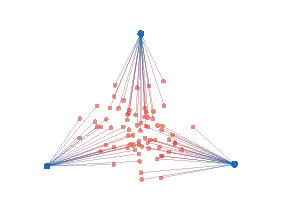
\includegraphics[width=.23\linewidth]{figures/generative-diffusion-versus-ot-2d/ot-rays.pdf} &
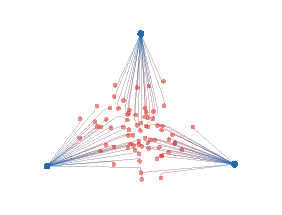
\includegraphics[width=.23\linewidth]{figures/generative-diffusion-versus-ot-2d/schedule-linear.pdf} &
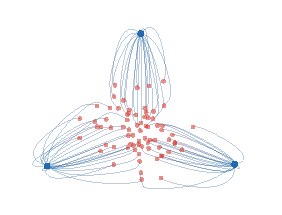
\includegraphics[width=.23\linewidth]{figures/generative-diffusion-versus-ot-2d/schedule-vp.pdf} &
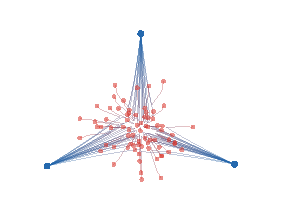
\includegraphics[width=.23\linewidth]{figures/generative-diffusion-versus-ot-2d/schedule-overshoot.pdf}
\end{tabular}}
\caption{\emph{Quadratic-OT rays and exact reverse-flow trajectories for three interpolants.} All four panels use the same three-Dirac target and centered Gaussian source. From left to right: straight displacement rays selected by quadratic OT; the linear bridge $a_t=1-t$, $b_t=t$; the variance-preserving OU bridge $a_\tau=e^{-\tau}$, $b_\tau=\sqrt{1-e^{-2\tau}}$; and the overshooting bridge $a_t=(1-t)(1-2t)$, $b_t=t$. The last bridge is not a time reparametrization of the preceding two and bends the trajectories more strongly.}
\index{Gaussian!mixture}% strictindex
\index{bridge!OU}% strictindex
\index{bridge!variance-preserving}% strictindex
\index{flow!probability ODE}% strictindex
\index{score function}% strictindex
\index{flow!reverse}% strictindex
\label{fig:generative-diffusion-schedule-comparison}
\end{figure}

\paragraph{Stochastic interpolants.}
\index{stochastic!interpolant}% strictindex
\index{latent!variable}% strictindex
\index{flow!probability ODE}% strictindex
The deterministic construction of Definition~\ref{def-deterministic-interpolant} can be enriched by a static Gaussian perturbation whose amplitude varies along the interpolation. In the construction of Albergo, Boffi and Vanden-Eijnden~\citep{Albergo2025StochasticInterpolants}, one auxiliary Gaussian variable is shared by the entire path.
\begin{defn}[Stochastic interpolant]\label{def-stochastic-interpolant}
Let $(X_0,X_1)\sim\pi\in\Couplings(\alpha_0,\alpha_1)$, let $Z\sim\Gaussian(0,\Id)$ be independent of $(X_0,X_1)$, and let $I_t$ be a deterministic interpolant for this coupling. Given an absolutely continuous noise schedule $\gamma:[0,1]\to\RR$ satisfying $\gamma(0)=\gamma(1)=0$, the stochastic interpolant is
\begin{equation}\label{eq-static-noise-stochastic-interpolant}
	X_t=I_t(X_0,X_1)+\gamma(t)Z,
	\qquad \alpha_t=\operatorname{Law}(X_t).
\end{equation}
Assume in addition that $\EE\int_a^b\norm{\partial_tI_t(X_0,X_1)+\dot\gamma(t)Z}^2\,\d t<+\infty$ for every $0<a<b<1$.
\end{defn}
The same draw of $Z$ is used for every $t$: conditionally on $(X_0,X_1,Z)$, the path remains absolutely continuous. Thus~\eqref{eq-static-noise-stochastic-interpolant} is the push-forward construction~\eqref{eq:interp-coupling} with latent variable $u=(X_0,X_1,Z)$. Its Eulerian velocity is
\[
	v_t(x)=\EE\bigl[\partial_tI_t(X_0,X_1)+\dot\gamma(t)Z\mid X_t=x\bigr],
\]
and Proposition~\ref{prop-flow-matching-vector-field}, applied on compact subintervals of $(0,1)$, gives the associated continuity equation. Local rather than endpoint-uniform square integrability includes the common schedule $\gamma(t)=\sqrt{t(1-t)}$, whose derivative is integrable but not square-integrable near the endpoints. The endpoint laws still follow by continuity of the interpolant. When regularity permits their construction, the associated SDEs are alternative dynamics with the same one-time marginals; they are not obtained by replacing $Z$ with independent noise at every time.

\begin{rem}[Brownian realizations of interpolant marginals]\label{rem-noisy-stochastic-interpolants}
\index{stochastic!interpolant}% strictindex
\index{Fokker-Planck@Fokker--Planck!equation}% strictindex
\index{flow!probability ODE}% strictindex
One can instead realize an interpolating marginal curve by Brownian-in-time dynamics. This gives a different path law from Definition~\ref{def-stochastic-interpolant}, although the one-time marginals can coincide, as in Proposition~\ref{prop-static-ou-equivalence}. The static-noise paths are absolutely continuous, whereas nondegenerate diffusion paths have nonzero quadratic variation. Let
\[
	\d X_t=r_t(U,X_t)\d t+\sigma_t(U,X_t)\d B_t,
	\qquad \alpha_t=\operatorname{Law}(X_t),
\]
where $U\sim\pi$ is static and independent of the Brownian motion $B_t$. Assume the SDE is well posed, adapted, and has locally integrable drift and quadratic variation so that the following It\^o calculation is justified. Conditioning on the observed state defines
\[
	v_t(x)=\EE\bigl[r_t(U,X_t)\mid X_t=x\bigr],
	\qquad
	D_t(x)=\EE\bigl[\sigma_t(U,X_t)\sigma_t(U,X_t)^\top\mid X_t=x\bigr].
\]
For smooth test functions $\varphi$,
\[
	\frac{\d}{\d t}\int\varphi\d\alpha_t
	=
	\int\dotp{\nabla\varphi}{v_t}\d\alpha_t
	+
	\frac12\int\tr(D_t\nabla^2\varphi)\d\alpha_t,
\]
or, in distributional form,
\begin{equation}\label{eq:noisy-interpolant-fokker-planck}
	\partial_t\alpha_t+\diverg(\alpha_tv_t)
	=
	\frac12\sum_{i,j}\partial_{i,j}^2\bigl((D_t)_{i,j}\alpha_t\bigr).
\end{equation}
The noisy analogue of~\eqref{eq:flow-matching} therefore regresses the drift through $\min_w\EE[\norm{w_t(X_t)-r_t(U,X_t)}^2]$. It learns a Fokker--Planck drift rather than a pure continuity-equation velocity. If $\alpha_t=\rho_t\d x$ has a smooth positive density, the same marginal curve has the formal probability-flow representation $\partial_t\rho_t+\diverg(\rho_t\bar v_t)=0$, where $\bar v_t=v_t-(2\rho_t)^{-1}\diverg(\rho_tD_t)$ and the matrix divergence is taken row-wise. For a spatially constant diffusion matrix $D_t(x)=\sigma_t^2\Id$, this becomes $\bar v_t=v_t-(\sigma_t^2/2)\nabla\log\rho_t$.
\index{flow!probability ODE}% strictindex
\end{rem}

% -----------------------------------------------------------------------------

\subsection{One-Step Generative Models}
\label{sec-one-step-generative-models}
\index{one-step generative model}% strictindex

One-step generative models try to keep the geometric training principle of flows while removing expensive multi-step integration at sampling time. To expose this tradeoff, we first describe direct non-parametric sampling by a Wasserstein flow; the subsequent constructions move that evolution into training and store its endpoint in a single generator evaluation.
\index{generative model}% strictindex

\paragraph{Non-parametric sampling via gradient flow.}
\index{Wasserstein!gradient flow}% strictindex
\index{particle!gradient flow}% strictindex
Let $\beta$ be the target law and let $\mathcal D\geq0$ be a discrepancy with $\mathcal D(\alpha,\beta)=0$ if and only if $\alpha=\beta$. Define
\begin{equation}\label{eq-one-step-discrepancy-energy}
	f_\beta(\alpha)\eqdef\mathcal D(\alpha,\beta).
\end{equation}
A direct sampling strategy follows the formal $\Wass_2$ gradient flow
\begin{equation}\label{eq-nonparametric-discrepancy-flow}
	\partial_t\alpha_t+\diverg(\alpha_t v_t)=0,
	\qquad
	v_t=-\Wgrad f_\beta(\alpha_t)
	=-\nabla\delta f_\beta(\alpha_t).
\end{equation}
If this flow is globally well posed and converges to a global minimizer of $f_\beta$, then its limit is $\beta$. These are substantial assumptions, not automatic consequences of the definition of a discrepancy. If $\alpha_0=n^{-1}\sum_{i=1}^n\delta_{X_i(0)}$ and the dynamics preserves empirical measures, then~\eqref{eq-nonparametric-discrepancy-flow} becomes the particle system
\begin{equation}\label{eq-nonparametric-particle-flow}
	\dot X_i(t)=v_t(X_i(t))
	=-\Wgrad f_\beta(\alpha_t)(X_i(t)),
	\qquad
	\alpha_t=\frac1n\sum_{i=1}^n\delta_{X_i(t)}.
\end{equation}
For fixed $n$, such a curve cannot converge weakly to a non-atomic target while retaining exactly $n$ equally weighted atoms. The sampling interpretation is therefore a large-particle approximation: one evolves a sufficiently rich cloud and lets $n$ increase. This approach is most practical in low dimension because it stores and repeatedly updates many interacting particles, in sharp contrast with flow matching, which learns a field that can subsequently transport arbitrary fresh samples.

For example, the squared Wasserstein loss moves a diffuse source toward the target along a time-reparametrized displacement interpolation. With an MMD loss, the interaction field derived in Section~\ref{sec-wasserstein-gradient-flows} instead moves particles according to kernel discrepancies. These choices give different trajectories even when the target law is the same; convergence must be studied for the chosen energy.

\paragraph{One-step models via parameter-domain discrepancy flows.}
\index{one-step generative model}% strictindex
\index{flow!parameter-domain}% strictindex
\index{discrepancy minimization}% strictindex
\index{minibatch bias}% strictindex
\index{parameter space}% strictindex
\index{minibatch}% strictindex
\index{Wasserstein!GAN}% strictindex
\index{MMD-GAN}% strictindex

The most direct one-step strategy is to train the generator parameters themselves by descending the discrepancy~\eqref{eq-one-step-discrepancy-energy}. Let $\zeta$ be a simple latent distribution and let $G_\theta:\Zz\to\RR^d$ be a neural generator on a standard Borel latent space $\Zz$. The objective is to find $\theta$ such that $(G_\theta)_\sharp\zeta=\beta$, or, in practice, such that the generated law is close to $\beta$. Define
\begin{equation}\label{eq-one-step-parameter-discrepancy}
	H_\beta(\theta)
	\eqdef
	f_\beta\big((G_\theta)_\sharp\zeta\big)
	=
	\mathcal D\big((G_\theta)_\sharp\zeta,\beta\big).
\end{equation}
This viewpoint includes Wasserstein GANs, MMD-GANs and Sinkhorn generative models~\citep{WassersteinGAN,MMD-GAN,2017-Genevay-AutoDiff}; when $\mathcal D$ is written through a dual potential or discriminator, it gives an adversarial formulation in which a discriminator represents that dual potential. The resulting training dynamics is the ordinary Euclidean gradient flow in parameter space,
\begin{equation}\label{eq-one-step-parameter-flow}
	\dot\theta_t=-\nabla_\theta H_\beta(\theta_t).
\end{equation}
This parameter flow induces a flow of generated measures, but this induced flow is not intrinsic in general. Set
\[
	\alpha_t\eqdef(G_{\theta_t})_\sharp\zeta,
	\qquad
	X_t=G_{\theta_t}(Z),
	\qquad
	Z\sim\zeta.
\]
\begin{prop}[Velocity induced by a parameter path]\label{prop-parameter-path-continuity}
	Assume that $t\mapsto\theta_t$ is continuously differentiable on $[0,T]$, and that, for $\zeta$-almost every $z$, the map $\theta\mapsto G_\theta(z)$ is continuously differentiable. Assume also that $(t,z)\mapsto\partial_\theta G_{\theta_t}(z)$ is jointly measurable and that
	\[
		\int_0^T\!\int_\Zz
		\norm{\partial_\theta G_{\theta_t}(z)\dot\theta_t}
		\,\d\zeta(z)\d t<+\infty.
	\]
	Let $\eta_{t,x}$ be a jointly measurable disintegration of $\d t\,\zeta(\d z)$ under $(t,z)\mapsto(t,G_{\theta_t}(z))$. Then the Eulerian velocity
	\begin{equation}\label{eq-one-step-induced-velocity}
		v_t(x)=\int \partial_\theta G_{\theta_t}(z)\dot\theta_t\,\d\eta_{t,x}(z)
	\end{equation}
		satisfies, in the distributional sense on $(0,T)\times\RR^d$,
	\begin{equation}\label{eq-one-step-induced-continuity}
		\partial_t\alpha_t+\diverg(\alpha_t v_t)=0.
	\end{equation}
	If $\theta_t$ follows~\eqref{eq-one-step-parameter-flow}, then $\dot\theta_t=-\nabla_\theta H_\beta(\theta_t)$ in~\eqref{eq-one-step-induced-velocity}.
\end{prop}

\begin{proof}
	The chain rule gives $\dot X_t=\partial_\theta G_{\theta_t}(Z)\dot\theta_t$. For every bounded measurable $\psi$, disintegration means
	\[
		\int \psi(z)\,\d\zeta(z)=\int_{\RR^d}\left(\int \psi(z)\,\d\eta_{t,x}(z)\right)\d\alpha_t(x)
	\]
	for almost every $t$. Consequently, for every smooth compactly supported $\varphi$,
	\[
		\frac{\d}{\d t}\int \varphi(x)\,\d\alpha_t(x)
		=
		\int \dotp{\nabla\varphi(x)}{v_t(x)}\,\d\alpha_t(x),
	\]
	which is the weak form of~\eqref{eq-one-step-induced-continuity}.
\end{proof}

The velocity~\eqref{eq-one-step-induced-velocity} depends on the parameter value $\theta_t$ and on the latent disintegration, not only on the measure $\alpha_t$. If the parametrization is non-identifiable, two different parameters can generate the same measure while inducing different velocities. Thus~\eqref{eq-one-step-parameter-flow} is a Euclidean gradient flow on parameter space, and only after push-forward a model-dependent flow on measures.
\index{continuity equation}% strictindex
\index{disintegration}% strictindex
\index{generator manifold}% strictindex
A practical difficulty is computing the gradient of $H_\beta$ from samples. One typically uses the minibatch law $\hat\beta_n=n^{-1}\sum_{i=1}^n\de_{Y_i}$, where $Y_i\overset{\mathrm{i.i.d.}}{\sim}\beta$, and replaces $H_\beta$ by the random objective $H_{\hat\beta_n}$. Unlike standard stochastic-gradient constructions, this substitution is not generally unbiased for nonlinear discrepancies:
\[
	\EE\left[\nabla_\theta H_{\hat\beta_n}(\theta)\right]
	\neq
	\nabla_\theta H_\beta(\theta).
\]
The expectation is over the data minibatch. This bias is a finite-sample effect of inserting the empirical measure inside a nonlinear transport or adversarial optimization before differentiating; it is distinct from the optimization noise of stochastic gradient descent. MMD losses admit unbiased $U$-statistic variants, but OT and entropic OT objectives generally exhibit finite-sample bias even when the underlying observations are unbiased.
\index{stochastic!gradient}% strictindex
\index{finite-sample bias}% strictindex
\index{empirical!measure}% strictindex

\paragraph{One-step models from Wasserstein flows.}
\index{Wasserstein!flow of discrepancy}% strictindex
\index{natural gradient}% strictindex
\index{flow!one-step}% strictindex
\index{Wasserstein!gradient flow}% strictindex

This construction keeps the same discrepancy but changes the geometry of descent. Instead of following its Euclidean gradient in parameter space, one approximates the intrinsic flow~\eqref{eq-nonparametric-discrepancy-flow} and fits each distribution-space update by a generator. This natural-gradient-type dynamics is less tied to a particular parametrization, although its convergence still depends on the geometry of $f_\beta$.

Let $\zeta$ be a simple latent distribution and let $\alpha_\theta=(G_\theta)_\sharp\zeta$ be the model distribution. Typical choices for $f_\beta$ include a smoothed relative entropy or an MMD loss, using the conventions of Section~\ref{sec-primer-functionals-discrepancies}. Writing its formal Wasserstein descent as
\index{maximum mean discrepancy}% strictindex
\begin{equation}\label{eq-one-step-wgf}
	\partial_t\al_t+\diverg(\al_t v_t)=0,
	\qquad
	v_t(x)=-\Wgrad f_\beta(\al_t)(x)
	=-\nabla\delta f_\beta(\al_t)(x),
\end{equation}
one fits, at each training time $t$, a parametric residual field $U_{\eta_t}$ along the current model distribution:
\begin{equation}\label{eq-one-step-l2-fit}
	\min_\eta \int
		\norm{U_\eta(x)-v_t(x)}^2
		\,\d\al_t(x).
\end{equation}
In a particle or generator implementation, the learned residual is then used to update the current generator by
\[
	\alpha_{\theta}^{+}
	=
	(\Id+\tau U_{\eta_t})_\sharp \alpha_\theta,
	\qquad\text{or equivalently}\qquad
	G_\theta^{+}(z)=G_\theta(z)+\tau U_{\eta_t}(G_\theta(z)).
\]
This is an ideal function-space update. If the residuals were stored as a growing composition, evaluation would still require one layer per training update and the model would not be one-step. A genuine one-step implementation therefore fits the updated outputs back into a fixed generator architecture, or distills the accumulated transport into one network, so that the final sampler remains a single evaluation of $G_\theta$.


After many training updates, the fixed-architecture or distilled generator is evaluated once at test time. W-Flow implements this principle with a Sinkhorn divergence, an entropy-regularized transport loss corrected by subtracting its self-costs~\citep{Han2026WFlow}; related constructions are studied in~\citet{He2026SinkhornDrifting}. We retain only the training mechanism here. The drifting models discussed below use the same fit-and-distill idea but prescribe a cheaper field that need not be an exact Wasserstein gradient.
\index{Wasserstein!gradient}% strictindex
\index{gradient!flow}% strictindex
\index{Wasserstein!gradient flow}% strictindex
\index{drifting!model}% strictindex

\paragraph{Drifting flows.}
\index{drifting!field}% strictindex

Computing the exact velocity in~\eqref{eq-one-step-wgf} can be costly. Drifting methods instead prescribe a cheaper distribution-correcting field, typically combining attraction toward the data with a self-normalization term, and regress it in $L^2(\al_t)$ as in~\eqref{eq-one-step-l2-fit}~\citep{Deng2026Drifting,Gretton2026DriftingWGF}. Such a field need not be the Wasserstein gradient of a fixed discrepancy. A simple continuous construction uses a strictly positive kernel $K_\epsilon(x,y)$ for which the following integrals are finite and defines, for every probability measure $\nu$,
\index{Wasserstein!gradient}% strictindex
\index{kernel!positive}% strictindex
\begin{equation}\label{eq-normalized-kernel-drift}
	B_\epsilon[\nu](x)
	\eqdef
	\frac{\int (y-x)K_\epsilon(x,y)\,\d\nu(y)}
	     {\int K_\epsilon(x,y)\,\d\nu(y)}.
\end{equation}
For the Gaussian kernel
\index{kernel!Gaussian}% strictindex
$K_\epsilon(x,y)=\exp(-\norm{x-y}^2/(2\epsilon))$, this normalized field is a score of a smoothed density:
\index{score function}% strictindex
\begin{equation}\label{eq-normalized-kernel-score}
	B_\epsilon[\nu](x)
	=
	\epsilon\nabla\log\!\left(\int K_\epsilon(x,y)\,\d\nu(y)\right).
\end{equation}
For this Gaussian kernel, the drifting velocity is
\begin{equation}\label{eq-cross-minus-self-drift}
	v_t(x)=B_\epsilon[\beta](x)-B_\epsilon[\al_t](x)
	=
	\epsilon\nabla\log
	\frac{\int K_\epsilon(x,y)\,\d\beta(y)}
	     {\int K_\epsilon(x,y)\,\d\al_t(y)}.
\end{equation}
The first term pulls samples toward data, while the second acts as a repulsive correction before coalescence. If all empirical particles occupy the same point, their self displacement is zero and they all receive the same target drift, so this deterministic field cannot recreate diversity. For fixed $\nu$, $B_\epsilon[\nu]$ is the Gaussian mean-shift displacement in~\eqref{eq-l2-attention-mean-shift}: it points from $x$ toward the local kernel barycenter of $\nu$. Thus~\eqref{eq-cross-minus-self-drift} subtracts the current model's mean-shift field from the target field.

Sampling follows the usual continuity equation $\partial_t\al_t+\diverg(\al_t v_t)=0$ from a prescribed simple law $\al_{t=0}=\al_0$; equivalently, particles solve $\dot X_i(t)=v_t(X_i(t))$. A direct implementation repeatedly evaluates~\eqref{eq-cross-minus-self-drift}. In a one-step implementation, the field is instead regressed by a neural network through~\eqref{eq-one-step-l2-fit}, and the accumulated evolution is fitted or distilled into the generator as described above. This moves the repeated integration cost from inference to training.
\index{kernel!norm}% strictindex


Figure~\ref{fig:generative-drifting-model-trajectories} gives a schematic comparison of two attraction-minus-weighted-self constructions; because several numerical choices differ, it should not be read as isolating the causal effect of one term.

\begin{figure}[ht]
\centering
\begin{tabular}{@{}cc@{}}
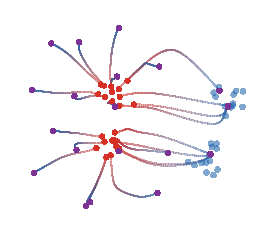
\includegraphics[width=.34\linewidth]{figures/generative-drifting-model-trajectories/unnormalized-trajectories.pdf} &
\index{drifting!model}% strictindex
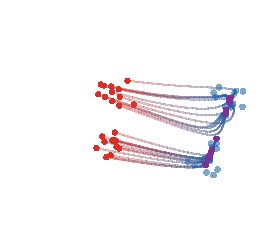
\includegraphics[width=.34\linewidth]{figures/generative-drifting-model-trajectories/normalized-trajectories.pdf}
\\[-.1em]
\small unnormalized Gaussian drift & \small normalized Gaussian drift
\index{self-corrected field}% strictindex
\end{tabular}
\caption{\emph{Two schematic Gaussian-kernel drifting trajectories for a small particle generator.} Both panels use attraction-minus-weighted-self fields. The left uses unnormalized Gaussian averages; the right uses normalized Gaussian mean-shift averages. Their target and self bandwidths, self weights, integration horizons and step sizes differ, and both simulations cap the instantaneous speed. The display compares two tuned constructions rather than a controlled ablation of self-repulsion.}
\label{fig:generative-drifting-model-trajectories}
\end{figure}

\subsection{Evolution in Depth of Transformers}
\label{sec-transformer-depth-evolution}
\index{transformer}% strictindex
\index{depth evolution}% strictindex

Deep residual architectures can be read as time discretizations of ODEs or PDEs. For transformers, the transported objects are token measures and the velocity is induced by attention.
\index{attention}% strictindex
\index{token measure}% strictindex

\paragraph{Tokens and mean-field attention.}
Transformers were introduced as sequence-to-sequence architectures driven by self-attention~\citep{Vaswani2017Attention} and have become central to language and vision models~\citep{Brown2020LanguageModels,Dosovitskiy2021Image}. After tokenization, embedding and any positional encoding, an input is represented by vectors \(x_1,\ldots,x_n\in\RR^d\), called \emph{tokens}. A transformer manipulates these vectors through a succession of attention, tokenwise neural-network and normalization layers. Attention is the principal mixing operation: it associates with each token a data-dependent weighted average of the value vectors carried by the full token population.
\index{positional encoding}% strictindex

Consider one attention head with parameters \(\theta=(Q,K,V)\), suppressing biases and the final output projection. Here \(Q,K\in\RR^{r\times d}\) are the query and key matrices and \(V\in\RR^{d\times d}\) is the value matrix. Thus \(Qx_i\) is the query carried by token \(i\), while \(Kx_j\) and \(Vx_j\) are the key and value carried by token \(j\). In the non-causal, unmasked setting used here, its discrete output is
\begin{equation}\label{eq-discrete-self-attention}
	\operatorname{Att}^{(n)}_\theta(x_1,\ldots,x_n)_i
	\eqdef
	\sum_{j=1}^n a_{i,j}(x_1,\ldots,x_n)Vx_j,
	\qquad
	a_{i,j}(x_1,\ldots,x_n)
	\eqdef
	\frac{\exp(\dotp{Qx_i}{Kx_j})}
	{\sum_{\ell=1}^n\exp(\dotp{Qx_i}{Kx_\ell})},
\end{equation}
Thus every query token may attend to every key token. Causal attention instead masks future indices; the resulting order dependence is deliberately omitted here. The conventional factor \(1/\sqrt r\) in the score can be absorbed into \(Q\) or \(K\).
\index{attention!non-causal}% strictindex
\index{attention!causal}% strictindex
\index{attention!masking}% strictindex

The map~\eqref{eq-discrete-self-attention} is permutation equivariant. Indeed, if \(\sigma\) is a permutation and \(x_i^\sigma=x_{\sigma(i)}\), reindexing the denominator gives \(a_{i,j}(x_1^\sigma,\ldots,x_n^\sigma)=a_{\sigma(i),\sigma(j)}(x_1,\ldots,x_n)\), and therefore
\[
	\operatorname{Att}^{(n)}_\theta(x_1^\sigma,\ldots,x_n^\sigma)_i
	=
	\operatorname{Att}^{(n)}_\theta(x_1,\ldots,x_n)_{\sigma(i)}.
\]
Relabeling the input tokens therefore only relabels the outputs. This statement concerns the already encoded token vectors: a causal mask or external position labels break this plain symmetry unless the position is retained as part of the token state. In the unmasked setting, permutation equivariance suggests replacing the ordered tuple by its empirical measure \(\al=n^{-1}\sum_{i=1}^n\de_{x_i}\).
\index{permutation!equivariance}% strictindex
\index{empirical!token measure}% strictindex


\begin{defn}[Mean-field attention map]\label{def-mean-field-attention-map}
\index{attention!mean-field map}% strictindex
	Fix \(p\geq1\), let $Q,K\in\RR^{r\times d}$ and $V\in\RR^{d\times d}$, write \(\theta=(Q,K,V)\), and let \(\al\in\Pp_p(\RR^d)\). Assume that, for \(\al\)-almost every \(x\),
	\[
		0<\int e^{\dotp{Qx}{Kz}}\,\d\al(z)<+\infty
		\qandq
		\int e^{\dotp{Qx}{Kz}}\norm{Vz}\,\d\al(z)<+\infty.
	\]
	The \emph{mean-field attention field} is
	\begin{equation}\label{eq-mean-field-attention}
		\Gamma_\theta[\al](x)
		\eqdef
		\frac{\int e^{\dotp{Qx}{Kz}}Vz\,\d\al(z)}
		{\int e^{\dotp{Qx}{Kz}}\,\d\al(z)}
	\end{equation}
	and, whenever \(\Gamma_\theta[\al]\in L^p(\al)\), the induced attention map on measures is
	\[
		\operatorname{Att}_\theta(\al)
		\eqdef
		(\Gamma_\theta[\al])_\sharp\al.
	\]
\end{defn}

These assumptions are automatic on compact supports. For $\alpha=n^{-1}\sum_i\delta_{x_i}$, one has $\Gamma_\theta[\alpha](x_i)=\operatorname{Att}^{(n)}_\theta(x_1,\ldots,x_n)_i$: the measure formulation is an exact rewriting, not an approximation. A many-token limit requires additional stability and compactness assumptions.

Here our principal limit concerns depth: the number $T$ of residual attention layers grows while each layer makes an update of size $1/T$, as in continuous-depth neural networks~\citep{Chen2018NeuralODE}. This is distinct from increasing the token count $n$. The whole current token law normalizes the attention weights, making the induced velocity nonlinear and context dependent. Related continuous-depth and Sinkhorn-normalized dynamics are studied in~\citet{Sander2022Sinkformers,Castin2025DynamicsTransformers}.
\index{continuous-depth neural network}% strictindex
\index{empirical!context}% strictindex
\index{attention!operator}% strictindex
\index{infinite-depth limit}% strictindex
\index{token limit}% strictindex
\index{transformer}% strictindex
\index{mean-field limit}% strictindex
\index{continuous!depth}% strictindex

We focus on the non-causal single-head mechanism of~\eqref{eq-discrete-self-attention}, ignoring MLP layers, layer normalization and masking. This stripped-down framework isolates the transport structure of a residual attention block.
\index{attention!single-head}% strictindex
\index{layer normalization}% strictindex
\index{causality}% strictindex
\index{masking}% strictindex
\index{transformer}% strictindex

\paragraph{Attention as a context-dependent velocity.}
\index{attention}% strictindex
\index{velocity field}% strictindex

We retain the notation \(\theta=(Q,K,V)\) and \(\Gamma_\theta\) of Definition~\ref{def-mean-field-attention-map}. Whereas~\eqref{eq-discrete-self-attention} replaces a token by its attention output, a residual block adds this output through a skip connection. With residual scale \(1/T\), it acts as
\begin{equation}\label{eq-transformer-residual-attention-step}
	x_i
	\longmapsto
	x_i+\frac1T\operatorname{Att}^{(n)}_\theta(x_1,\ldots,x_n)_i
	=
	x_i+\frac1T
	\sum_{j=1}^n
	\frac{e^{\dotp{Qx_i}{Kx_j}}Vx_j}
	{\sum_{\ell=1}^n e^{\dotp{Qx_i}{Kx_\ell}}}.
\end{equation}
The attention output is therefore interpreted as a context-dependent velocity, and the skip connection performs one explicit Euler step along this field.
\index{skip connection}% strictindex
\index{explicit Euler scheme}% strictindex

\paragraph{Token measure evolution.}
\index{residual attention}% strictindex
\index{in-context map}% strictindex
\index{token measure}% strictindex

Let \(x_i^{(\ell)}\) be token \(i\) after layer \(\ell\), and let \(\al^{(\ell)}=n^{-1}\sum_i\de_{x_i^{(\ell)}}\) be the corresponding empirical law. With \(\tau=1/T\), equation~\eqref{eq-transformer-residual-attention-step} is exactly
\begin{equation}\label{eq-transformer-residual-measure-step}
	\al^{(\ell+1)}
	=
	\left(
		\Id+\tau\Gamma_{\theta^{(\ell)}}[\al^{(\ell)}]
	\right)_\sharp
	\al^{(\ell)},
	\qquad
	\ell=0,\ldots,T-1.
\end{equation}
Unlike the non-residual map \(\operatorname{Att}_\theta\) of Definition~\ref{def-mean-field-attention-map}, this update keeps each current token and adds a small attention displacement.
\index{empirical!measure}% strictindex
\index{transformer}% strictindex
Set \(t_\ell=\ell/T\) and suppose that \(\theta^{(\ell)}\) samples a sufficiently regular depth-dependent path \(t\mapsto\theta_t\). As \(T\to+\infty\), a time interpolation of~\eqref{eq-transformer-residual-measure-step} converges formally to the conservation equation
\begin{equation}\label{eq-transformer-mean-field-pde}
	\partial_t\al_t
	+
	\diverg\!\left(\al_t\Gamma_{\theta_t}[\al_t]\right)
	=
	0.
\end{equation}



\paragraph{$L^2$ attention and mean shift.}
\index{L2 self-attention@$L^2$ self-attention}% strictindex
\index{mean-shift PDE}% strictindex
\index{kernel!regression}% strictindex
\index{attention!Gaussian kernel}% strictindex
\index{mean shift}% strictindex

A particularly geometric variant replaces the dot-product score \(\dotp{Qx}{Ky}\) by a negative squared Euclidean score \(s_\epsilon(x,y)=-\norm{x-y}^2/(2\epsilon)\). Take, for simplicity, the same token space for queries, keys and values, and set
\[
	K_\epsilon(x,y)=\exp(-\norm{x-y}^2/(2\epsilon)),
	\qquad
	\rho_\epsilon[\alpha](x)=\int K_\epsilon(x,y)\d\alpha(y),
	\qquad
	m_\epsilon[\alpha](x)
	=
	\frac{\int yK_\epsilon(x,y)\d\alpha(y)}
	     {\rho_\epsilon[\alpha](x)}.
\]
The map $x\mapsto m_\epsilon[\alpha](x)$ is exactly Gaussian-kernel attention, i.e.\ normalized kernel regression over tokens; such $L^2$ or Gaussian-kernel scores are used explicitly in transformer variants motivated by Lipschitz control and projection-free attention~\citep{KimPapamakariosMnih2020L2SelfAttention,KunduGhoshGhoshHonavar2026GaussianKernelAttention}. Classical mean shift, however, uses the displacement from the current point to this local barycenter. This gives
\index{L2 attention@$L^2$ attention}% strictindex
\index{projection-free attention}% strictindex
\begin{equation}\label{eq-l2-attention-mean-shift}
	M_\epsilon[\alpha](x)
	\eqdef
	m_\epsilon[\alpha](x)-x
	=
	\frac{\int (y-x)K_\epsilon(x,y)\d\alpha(y)}
	     {\rho_\epsilon[\alpha](x)}
	=
	\epsilon\nabla\log\rho_\epsilon[\alpha](x)
\end{equation}
and, when $\alpha$ is empirical, $\rho_\epsilon[\alpha]$ is a Gaussian kernel density estimate up to normalization. Thus \(M_\epsilon[\alpha]\) is the classical Gaussian mean-shift vector~\citep{FukunagaHostetler1975,Cheng1995MeanShift,ComaniciuMeer2002MeanShift}. If the data measure $\alpha$ is frozen, the update $x\leftarrow m_\epsilon[\alpha](x)$ is the usual mode-seeking mean-shift iteration. If instead all support points move and the empirical measure is recomputed after every step, one obtains the self-consistent, or \emph{blurring}, mean-shift process~\citep{Chen2015BlurringMeanShift}. Its damped update is
\index{mean shift!blurring}% strictindex
\index{kernel!density estimate}% strictindex
\index{mean shift!vector}% strictindex
\[
	x_i^{(\ell+1)}
	=
	(1-\tau)x_i^{(\ell)}+\tau m_\epsilon[\alpha^{(\ell)}](x_i^{(\ell)})
	=
	x_i^{(\ell)}+\tau M_\epsilon[\alpha^{(\ell)}](x_i^{(\ell)})
\]
which is an explicit Euler step of the continuous-time mean-shift equation
\[
	\partial_t\alpha_t+\diverg\bigl(\alpha_tM_\epsilon[\alpha_t]\bigr)=0.
\]
For $\tau=1$ this is discrete blurring mean shift; for small $\tau$ it approximates a transport PDE that moves each token uphill along the log of the smoothed token density. This distinction between the raw barycentric attention output $m_\epsilon$ and the velocity $M_\epsilon=m_\epsilon-\Id$ is important: adding $m_\epsilon$ directly as a residual would produce a different drift. The mean-shift form isolates a purely metric attention mechanism from the learned bilinear geometry of $\dotp{Qx}{Ky}$.
\index{mean shift!iteration}% strictindex
\index{barycentric!attention}% strictindex

\begin{rem}[Consensus for blurring mean shift]\label{rem-mean-shift-consensus}
\index{opinion dynamics}% strictindex
\index{consensus}% strictindex
\index{clustering}% strictindex
\index{bounded confidence}% strictindex
\index{mean shift!blurring}% strictindex
The self-consistent mean-shift equation is a continuum consensus model. If $\alpha_0$ is compactly supported and the interaction kernel is positive and Lipschitz on the convex hull of its support, that hull is forward invariant and the normalized averaging kernels share a uniform positive fraction of mass. This common contribution contracts each directional width of the moving support, and hence its diameter. Under the corresponding characteristic well-posedness assumptions, it yields exponential contraction of the support diameter and convergence of $\alpha_t$ in every $\Wass_p$, $1\leq p<+\infty$, to a Dirac mass; see~\citet{HegselmannKrause2002OpinionDynamics,Chen2015BlurringMeanShift,MotschTadmor2014Heterophilious} and the finite-agent and Eulerian consensus analyses in~\citet{BlondelHendrickxTsitsiklis2009Krause,CanutoFagnaniTilli2012EulerianKrause}. Without strict positivity, consensus is no longer guaranteed: bounded-confidence kernels can disconnect the interaction graph and produce several clusters instead of one consensus point. Moreover, because the normalized interactions are generally asymmetric, the limiting point need not be the initial barycenter.
\end{rem}

Figure~\ref{fig:generative-mean-shift-pde} visualizes the long transient before this eventual consensus: particles climb the current smoothed density while the density itself sharpens.

\begin{figure}[htbp]
\centering
\begin{tabular}{@{}c@{\hspace{.5em}}c@{}}
\raisebox{-.5\height}{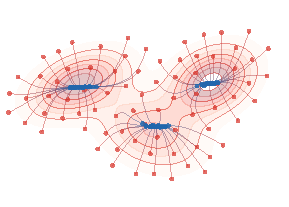
\includegraphics[width=.39\linewidth]{figures/generative-mean-shift-pde/trajectories.pdf}} &
\begin{tabular}{@{}cc@{}}
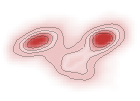
\includegraphics[width=.185\linewidth]{figures/generative-mean-shift-pde/snapshot-1.pdf} &
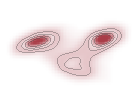
\includegraphics[width=.185\linewidth]{figures/generative-mean-shift-pde/snapshot-2.pdf} \\
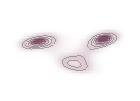
\includegraphics[width=.185\linewidth]{figures/generative-mean-shift-pde/snapshot-3.pdf} &
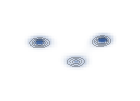
\includegraphics[width=.185\linewidth]{figures/generative-mean-shift-pde/snapshot-4.pdf}
\end{tabular}
\\[-.2em]
\small trajectories on the initial density & \small later density snapshots
\end{tabular}
\caption{\emph{Continuous-time mean shift for a densely sampled three-Gaussian mixture.} Left: initial density level sets, in red, and representative particle paths of $\dot x=M_\epsilon[\alpha_t](x)$, colored from red to blue. Right: four later kernel-density renderings of $\alpha_t$ at increasing times, with the same red-to-blue time palette; the initial density is omitted because it is shown on the left. The snapshots show the long multimodal transient before the globally positive Gaussian interactions drive the cloud toward the one-point consensus described in Remark~\ref{rem-mean-shift-consensus}.}
\label{fig:generative-mean-shift-pde}
\end{figure}
\index{kernel!Gaussian}% strictindex
\index{kernel!regression}% strictindex
\index{transport!PDE}% strictindex

\paragraph{Gradient structure and limitations.}
\index{gradient!structure}% strictindex

When the token space has dimension $d$ and the query/key space has dimension $r$, take $Q,K\in\RR^{r\times d}$ and $V\in\RR^{d\times d}$. Assume compact token support, or sufficient exponential-moment bounds to justify differentiation under the integrals below. If $V=Q^\top K$, the field $\Gamma_\theta[\alpha]$ is a gradient vector field in the token variable. Indeed, define the log-partition potential
\[
	\Phi_\alpha(x)
	=
	\int \exp(\dotp{Qx}{Ky})\d\alpha(y),
	\qquad
	U_\alpha(x)=\log\Phi_\alpha(x).
\]
Then
\[
	\nabla_x U_\alpha(x)
	=
	\frac{\int Q^\top K y\,\exp(\dotp{Qx}{Ky})\d\alpha(y)}
	     {\int \exp(\dotp{Qx}{Kz})\d\alpha(z)}
	=
	\Gamma_\theta[\alpha](x).
\]
This proves only that the velocity is an instantaneous gradient in $x$; it does not by itself identify a Wasserstein energy. Indeed, the natural scalar candidate $f_{\rm att}(\alpha)=\int U_\alpha(x)\,\d\alpha(x)$ has first variation
\[
	\delta f_{\rm att}(\alpha)(z)
	=
	U_\alpha(z)
	+
	\int
	\frac{\exp(\dotp{Qx}{Kz})}{\Phi_\alpha(x)}
	\,\d\alpha(x),
\]
up to an additive constant. The second term is the response of every query normalization to a perturbation of the key distribution, and its spatial gradient is absent from $\Gamma_\theta[\alpha]$. Thus, without additional symmetry or integrability conditions, the displayed attention PDE is a transportation dynamics rather than the Wasserstein gradient flow of this fixed scalar functional. Special variants recover additional structure: Sinkhorn attention can be interpreted through doubly stochastic normalization and Wasserstein-type gradient flows~\citep{Sander2022Sinkformers,Castin2025DynamicsTransformers}, while layer normalization leads naturally to dynamics on the sphere and to modified metrics. The key open difficulty for the present viewpoint is training: after the architecture has been rewritten as a controlled transport equation, learning corresponds to optimizing the time-dependent parameters $(\theta_t)_t$ rather than merely analyzing the forward PDE for fixed parameters.
\index{transformer}% strictindex
\index{doubly stochastic normalization}% strictindex
\index{transport!equation}% strictindex
\index{controlled transport}% strictindex
\index{first variation}% strictindex
\index{layer normalization}% strictindex
\index{Wasserstein!gradient}% strictindex
\index{gradient!flow}% strictindex
\index{Wasserstein!gradient flow}% strictindex
\index{attention}% strictindex

\subsection{Flows over the Gaussian Manifold}
\label{sec-gaussian-closure-transport-dynamics}
\index{Gaussian!manifold}% strictindex

Gaussian measures provide a useful testing ground for the preceding dynamics. They are not invariant under a general Wasserstein gradient flow: a nonlinear velocity usually creates non-Gaussian densities immediately. The useful substitute is to either identify affine velocities, which exactly preserve Gaussianity, or to project the dynamics onto the Gaussian manifold. In both cases the measure PDE reduces to matrix ODEs for the mean and covariance. This viewpoint is emphasized in the survey~\citep{Peyre2026OptimalDiffusionTransports} and is useful for comparing diffusion paths, Wasserstein gradient flows, drifting fields and transformer-type dynamics.
\index{affine!closure}% strictindex
\index{drifting!field}% strictindex
\index{Wasserstein!gradient}% strictindex
\index{gradient!flow}% strictindex
\index{transformer}% strictindex
\index{Wasserstein!gradient flow}% strictindex
\index{Gaussian!manifold}% strictindex
\index{Gaussian!measure}% strictindex

For constrained gradient flows on this family, the covariance equation is the finite-dimensional Bures--Wasserstein gradient flow on positive definite matrices. This restricted metric is the same in both settings, but exact ambient preservation and deliberate projection onto the submanifold remain distinct claims. Figure~\ref{fig:gradflow-gaussian-closure} first compares two illustrative Gaussian paths from a source \(\alpha_0\) to a target \(\gamma\); the exact ambient equations admitting Gaussian solutions for specified energies \(f(\alpha)\) are catalogued afterwards in Proposition~\ref{prop-centered-gaussian-covariance-catalogue}.
\index{Gaussian!submanifold}% strictindex
\index{affine!gradient}% strictindex
\index{Bures!Wasserstein geometry}% strictindex
\index{Wasserstein!gradient}% strictindex
\index{Gaussian!closure}% strictindex
\index{gradient!flow}% strictindex

\begin{figure}[ht]
\centering
\begin{tabular}{@{}c@{\hspace{1.5em}}c@{}}
\small $\Wass_2$ geodesic & \small drifting closure \\[-.15em]
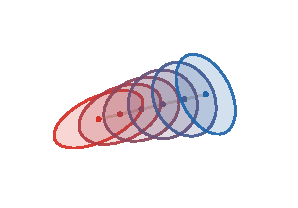
\includegraphics[width=.30\linewidth]{figures/gradflow-gaussian-closure/ot-ellipses.pdf} &
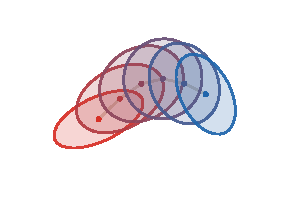
\includegraphics[width=.30\linewidth]{figures/gradflow-gaussian-closure/drifting-ellipses.pdf}
\end{tabular}
\caption{\emph{Two Gaussian paths from a red source $\alpha_0$ to a blue target $\gamma=\Gaussian(\bar m,\bar\Sigma)$.} The left panel is the constant-speed $\Wass_2$ geodesic minimizing the Benamou--Brenier action. The right panel is a prescribed non-variational drifting flow with an affine Gaussian-preserving velocity: its mean follows a curved path while its covariance reaches the same endpoint.}
\index{moment matching}% strictindex
\index{Gaussian!closure}% strictindex
\index{velocity field}% strictindex
\label{fig:gradflow-gaussian-closure}
\end{figure}

\paragraph{Gaussianity preservation.}
\index{Gaussian!preservation}% strictindex

The first question is invariance: one wants a simple criterion ensuring that the continuity equation does not leave the finite-dimensional Gaussian family.
\index{continuity equation}% strictindex


\begin{prop}[Affine velocities preserve Gaussianity]\label{prop-gaussian-affine-closure}
\index{affine!closure}% strictindex
	Let $\alpha_0=\Gaussian(m_0,\Sigma_0)$, with $\Sigma_0\succ0$. Let $b_t\in\RR^d$ and $A_t\in\RR^{d\times d}$ be locally integrable on a time interval, and let $(m_t,\Sigma_t)$ solve
	\[
		\dot m_t=b_t,
		\qquad
		\dot\Sigma_t=A_t\Sigma_t+\Sigma_tA_t^\top,
		\qquad
		(m_{t=0},\Sigma_{t=0})=(m_0,\Sigma_0).
	\]
	Then, as long as this matrix ODE is defined, $\Sigma_t\succ0$ and
	\[
		\alpha_t=\Gaussian(m_t,\Sigma_t)
	\]
	is the solution of the continuity equation
	\[
		\partial_t\alpha_t+\diverg(\alpha_t v_t)=0,
		\qquad
		v_t(x)=b_t+A_t(x-m_t).
	\]
	In particular, if a smooth functional $f$ has a Wasserstein gradient on Gaussian measures of the affine form
	\[
		\Wgrad f(\Gaussian(m,\Sigma))(x)
		=
		b_f(m,\Sigma)+A_f(m,\Sigma)(x-m),
	\]
	with $A_f(m,\Sigma)$ symmetric, then the displayed moment ODE below produces a Gaussian distributional solution of the full Wasserstein gradient-flow equation for $f$:
	\[
		\dot m_t=h_f(m_t,\Sigma_t),
		\qquad
		\dot\Sigma_t=H_f(m_t,\Sigma_t),
	\]
	where
	\[
		h_f(m,\Sigma)=-b_f(m,\Sigma),
		\qquad
		H_f(m,\Sigma)
		=
		-\bigl(A_f(m,\Sigma)\Sigma+\Sigma A_f(m,\Sigma)\bigr).
	\]
	Conversely, fix a non-degenerate Gaussian \(\Gaussian(m,\Sigma)\). Suppose that a finite-energy Wasserstein tangent field \(V_{m,\Sigma}\) is represented by a gradient in \(L^2(\Gaussian(m,\Sigma))\) and is tangent to the Gaussian manifold at this Gaussian. Then there exist \(b(m,\Sigma)\) and a symmetric matrix \(A(m,\Sigma)\) such that
	\[
		V_{m,\Sigma}(x)=b(m,\Sigma)+A(m,\Sigma)(x-m)
		\qquad
		\Gaussian(m,\Sigma)\text{-a.e.}
	\]
	Consequently, under the same smoothness assumptions, if the Wasserstein gradient flow of a functional preserves the Gaussian family for all non-degenerate Gaussian initial data, then \(\Wgrad f(\Gaussian(m,\Sigma))\) is affine on each Gaussian. Without the Wasserstein gradient representative, this converse is false because one may add velocity fields with zero \(\Gaussian(m,\Sigma)\)-weighted divergence.
\index{affine!closure}% strictindex
\index{Wasserstein!gradient}% strictindex
\index{Gaussian!manifold}% strictindex
\index{divergence-free field}% strictindex

	Finally, any smooth Gaussian curve with positive definite covariance can be generated by an affine velocity. If one wants the velocity to be a Wasserstein tangent gradient, one chooses the unique symmetric solution of the Lyapunov equation
\index{affine!closure}% strictindex
\index{Lyapunov equation}% strictindex
	\[
		A_t\Sigma_t+\Sigma_t A_t=\dot\Sigma_t.
	\]
\end{prop}

\begin{proof}
	Let \(X_t\) follow the characteristic ODE \(\dot X_t=b_t+A_t(X_t-m_t)\) with \(X_0\sim\Gaussian(m_0,\Sigma_0)\). Since \(\dot m_t=b_t\), the centered variable \(\tilde X_t=X_t-m_t\) solves the homogeneous linear ODE \(\dot{\tilde X}_t=A_t\tilde X_t\). If \(\Phi_t\) is the fundamental matrix \(\dot\Phi_t=A_t\Phi_t\), \(\Phi_{t=0}=\Id\), then
	\[
		X_t=m_t+\Phi_t(X_0-m_0),
		\qquad
		\Sigma_t=\Phi_t\Sigma_0\Phi_t^\top.
	\]
	Hence \(X_t\) is Gaussian and \(\Sigma_t\succ0\), and
\index{random variable}% strictindex
	\[
		\dot\Sigma_t
		=
		\frac{\d}{\d t}\EE\bigl(\tilde X_t\tilde X_t^\top\bigr)
		=
		A_t\Sigma_t+\Sigma_t A_t^\top.
	\]
	This proves Gaussian preservation and the moment ODE\@. The Wasserstein gradient-flow statement follows by inserting the descent velocity $v_t=-\Wgrad f(\alpha_t)$.
\index{Wasserstein!gradient}% strictindex

	For the converse, fix $\alpha=\Gaussian(m,\Sigma)$ and denote its density by $\rho$. Tangency to the Gaussian manifold means that the density variation $-\diverg(\rho V)$ is generated by some moment variation $(\dot m,\dot\Sigma)$, with $\dot\Sigma$ symmetric. Set $b=\dot m$, and let $A=A^\top$ be the unique solution of
	\(A\Sigma+\Sigma A=\dot\Sigma\).
	By the first part of the proposition, the affine gradient field $V_0(x)=b+A(x-m)$ generates exactly the same infinitesimal Gaussian variation. Hence
	\(\diverg\bigl(\rho(V-V_0)\bigr)=0\)
	in the distributional sense. Both $V$ and $V_0$ belong to the $L^2(\alpha)$ closure of gradient fields. The weighted Helmholtz decomposition therefore makes $V-V_0$ simultaneously a tangent gradient and orthogonal to every tangent gradient, so $V=V_0$ in $L^2(\alpha)$. Equivalently, for a smooth representative $V-V_0=\nabla\psi$, integration by parts gives $\int\norm{\nabla\psi}^2\d\alpha=0$. This proves that the Wasserstein tangent representative is affine. The qualification is essential: without selecting the gradient representative, one can add a nonzero field with zero $\alpha$-weighted divergence without changing the Gaussian curve.
\index{Helmholtz decomposition}% strictindex

	For a prescribed smooth Gaussian curve, set $b_t=\dot m_t$ and choose any matrix $A_t$ satisfying $A_t\Sigma_t+\Sigma_tA_t^\top=\dot\Sigma_t$. Since $\Sigma_t$ is positive definite, the Lyapunov map $A\mapsto A\Sigma_t+\Sigma_t A$ is invertible on symmetric matrices, which gives the unique symmetric choice when a gradient velocity is required. In that case $v_t$ is the gradient of the quadratic potential $x\mapsto \dotp{b_t}{x}+\dotp{A_t(x-m_t)}{x-m_t}/2$.
\index{quadratic!potential}% strictindex
\index{gradient!velocity}% strictindex
\end{proof}

\paragraph{Gaussian-preserving gradient flows.}
\index{Gaussian!preservation}% strictindex
\index{gradient!flow}% strictindex

We now instantiate the affine-gradient viewpoint by tracking functionals whose full Wasserstein gradient is affine on Gaussian inputs. The catalogue below gives exact Gaussian solutions of the ambient Wasserstein equations, not projected or constrained flows. Whenever the ambient equation is unique in the solution class under consideration, this solution is the selected Wasserstein gradient flow and proves invariance of the Gaussian family; without such a uniqueness theorem, it still proves existence of a Gaussian distributional solution, but not invariance of every weak solution.
\index{Wasserstein!gradient}% strictindex
\index{moment functional}% strictindex

\begin{prop}[Gaussian closure catalogue]\label{prop-centered-gaussian-covariance-catalogue}
\index{Gaussian!covariance}% strictindex
\index{Gaussian!mean}% strictindex
\index{Gaussian!manifold}% strictindex
	In the moment-functional row, assume $g$ is continuously differentiable in $(m,\Sigma)$. Let \(\gamma=\Gaussian(\bar m,\bar\Sigma)\) on \(\RR^d\), with \(\bar\Sigma\succ0\), and let the initial condition be \(\alpha_0=\Gaussian(m_0,\Sigma_0)\), with \(\Sigma_0\succ0\). For each functional displayed below, evaluating its ambient Wasserstein gradient on a Gaussian gives an affine field. Consequently, as long as the following finite-dimensional ODE exists and \(\Sigma_t\succ0\),
	\[
		\alpha_t=\Gaussian(m_t,\Sigma_t)
	\]
	is an exact distributional solution of the corresponding ambient gradient-flow PDE, and its mean and covariance satisfy
	\[
		\dot{m}_t=h(m_t,\Sigma_t),
		\qquad
		\dot{\Sigma}_t=H(m_t,\Sigma_t).
	\]
	Write \(\delta_m=m-\bar m\), \(A=\bar\Sigma^{-1}\), and
	\[
		M_{\Sigma,\bar\Sigma}
		\eqdef
		\Sigma^{-1/2}\bigl(\Sigma^{1/2}\bar\Sigma\Sigma^{1/2}\bigr)^{1/2}\Sigma^{-1/2}.
	\]
	The relative Fisher information, used only as an energy in this catalogue, is
	\[
		\mathcal I(\alpha|\gamma)
		=
		\int \left|\nabla\log\frac{\rho(x)}{\rho_\gamma(x)}\right|^2\rho(x)\,\d x
		=
		\int
		\left|\nabla\log\rho(x)+A(x-\bar m)\right|^2\rho(x)\,\d x
		\qquad(\alpha=\rho\,\d x),
	\]
	where $\rho$ is smooth and positive and $\rho_\gamma$ is the density of $\gamma$. For the MMD row, set $R=\Sigma+m\,m^\top-\bar\Sigma-\bar m\,\bar m^\top$.
	With the normalizations displayed in the first column, the mean vector field \(h\) and covariance vector field \(H\) are listed in the following table. If that PDE is unique in the selected solution class, this Gaussian solution is the Wasserstein flow from \(\alpha_0\). Gradients with respect to \(\Sigma\) are symmetric Frobenius gradients on the cone of covariance matrices.
	\index{maximum mean discrepancy}% strictindex
		\begin{center}
		\begingroup
		\small
		\renewcommand{\arraystretch}{1.55}
		\begin{tabularx}{\linewidth}{>{\raggedright\arraybackslash}p{.42\linewidth}>{\centering\arraybackslash}p{.18\linewidth}>{\raggedright\arraybackslash}X}
			\hline
			Functional \(f(\alpha)\) & \(h(m,\Sigma)\) & \(H(m,\Sigma)\) \\
			\hline
			\(g(m_\alpha,\Sigma_\alpha)\)
			&
			\(-\nabla_m g\)
			&
			\(-2(\Sigma\nabla_\Sigma g+\nabla_\Sigma g\,\Sigma)\)
			\\
			\(\displaystyle \int\Bigl(\frac12x^\top Bx+\dotp{\ell}{x}\Bigr)\d\alpha(x)\), \(B=B^\top\)
			&
			\(-(B m+\ell)\)
			&
			\(-(\Sigma B+B\Sigma)\)
			\\
			\(\displaystyle \frac14\iint (x-y)^\top G(x-y)\d\alpha(x)\d\alpha(y)\), \(G=G^\top\)
			&
			\(0\)
			&
			\(-(\Sigma G+G\Sigma)\)
			\\
			\(\KL(\alpha|\gamma)\)
			&
			\(-A\delta_m\)
			&
			\(2\Id-\Sigma A-A\Sigma\)
			\\
			\(\mathcal I(\alpha|\gamma)\)
			&
			\(-2A^2\delta_m\)
			&
			\(4\Sigma^{-1}-2\Sigma A^2-2A^2\Sigma\)
			\\
			\(\Wass_2^2(\alpha,\gamma)\)
			&
			\(-2\delta_m\)
			&
			\(2(M_{\Sigma,\bar\Sigma}\Sigma+\Sigma M_{\Sigma,\bar\Sigma}-2\Sigma)\)
			\\
			\(\MMD_k^2(\alpha,\gamma)\), \(k(x,y)=\dotp{x}{y}^2\)
			&
			\(-4R m\)
			&
			\(-4(\Sigma R+R\Sigma)\)
			\\
			\hline
		\end{tabularx}
		\endgroup
		\end{center}
\end{prop}

\begin{proof}
	For the moment-functional row, the formula is exact on the full Wasserstein space. Indeed, write $m_\alpha=\int x\,\d\alpha(x)$ and $\Sigma_\alpha=\int (x-m_\alpha)(x-m_\alpha)^\top\d\alpha(x)$. If \(\eta\) is a signed perturbation with zero total mass, then $\d m_\alpha[\eta]=\int x\,\d\eta(x)$ and $\d\Sigma_\alpha[\eta]=\int (x-m_\alpha)(x-m_\alpha)^\top\d\eta(x)$. Thus, up to an irrelevant additive constant, the first variation is $\delta f(\alpha)(x)=\dotp{\nabla_m g}{x}+\dotp{\nabla_\Sigma g}{(x-m_\alpha)(x-m_\alpha)^\top}$,
	and its spatial gradient is the affine field
	\[
		\nabla_x\delta f(\alpha)(x)
		=
		\nabla_m g+2\nabla_\Sigma g\,(x-m_\alpha).
	\]
	Consequently the full Wasserstein descent velocity is affine, and Proposition~\ref{prop-gaussian-affine-closure} gives the displayed moment equations.
\index{moment functional}% strictindex
\index{first variation}% strictindex

	For the quadratic potential row, the ambient first variation is
	\[
		\delta f(\alpha)(x)=\frac12x^\top Bx+\dotp{\ell}{x},
		\qquad
		\nabla_x\delta f(\alpha)(x)=B m+\ell+B(x-m),
	\]
	which gives the displayed affine velocity. For the quadratic interaction row, the ambient first variation is $\delta f(\alpha)(x)=\frac12\int (x-y)^\top G(x-y)\d\alpha(y)$, with $\nabla_x\delta f(\alpha)(x)=G(x-m_\alpha)$.
	These first variations are quadratic in \(x\), hence the affine Gaussian flow coincides with the full Wasserstein gradient flow.
\index{quadratic!potential}% strictindex
\index{energy!interaction}% strictindex
\index{first variation}% strictindex

	For the KL row, write $\alpha=\rho\,\d x$ and let $\rho_\gamma$ denote the density of $\gamma$. The ambient first variation is \(\log(\rho/\rho_\gamma)\) up to an additive constant. If \(\alpha=\Gaussian(m,\Sigma)\), then
	\[
		\nabla\log(\rho/\rho_\gamma)(x)
		=
		-\Sigma^{-1}(x-m)+A(x-\bar m),
	\]
	so the descent velocity is
	\(v(x)=-A\delta_m+(\Sigma^{-1}-A)(x-m)\).
	Proposition~\ref{prop-gaussian-affine-closure} gives \(h(m,\Sigma)=-A\delta_m\) and \(H(m,\Sigma)=2\Id-\Sigma A-A\Sigma\). For the Fisher row, writing \(u=\log(\rho/\rho_\gamma)\), the ambient first variation of \(\frac12\mathcal I(\alpha|\gamma)\) is, up to constants,
	\[
		-\Delta u-\frac12|\nabla u|^2-\dotp{\nabla u}{\nabla\log\rho_\gamma}.
	\]
	For Gaussian \(\rho\) and Gaussian \(\gamma\), this is quadratic in \(x\). Multiplying by two for \(\mathcal I(\alpha|\gamma)\) gives the descent velocity
	\[
		v(x)=-2A^2\delta_m+2(\Sigma^{-2}-A^2)(x-m).
	\]
	Hence the Wasserstein velocity is affine and the Gaussian family is closed, with the displayed \(h\) and \(H\). Although the ambient Fisher flow is a fourth-order PDE for a generic density, it is therefore an exact finite-dimensional closure in this quadratic-reference case.
\index{Kullback-Leibler@Kullback--Leibler!divergence}% strictindex
\index{Fisher information}% strictindex

	For \(\Wass_2^2(\alpha,\gamma)\), the Brenier map from \(\Gaussian(m,\Sigma)\) to \(\gamma\) is
	\(T(x)=\bar m+M_{\Sigma,\bar\Sigma}(x-m)\).
	The descent velocity for the unhalved squared distance is \(2(T-\Id)\), which gives the mean and covariance equations through Proposition~\ref{prop-gaussian-affine-closure}. For the MMD row, \(k(x,y)=\dotp{x}{y}^2\) identifies the kernel mean embedding with the raw second moment. Thus
	\[
		\MMD_k^2(\alpha,\gamma)
		=
		\norm{\Sigma+m\,m^\top-\bar\Sigma-\bar m\,\bar m^\top}_{\mathrm F}^2
		=
		\norm{R}_{\mathrm F}^2,
	\]
	and the ambient first variation is \(2x^\top R x\), whose descent velocity is \(-4Rx\). This gives \(h(m,\Sigma)=-4R m\) and \(H(m,\Sigma)=-4(\Sigma R+R\Sigma)\).
\index{Brenier!map}% strictindex
\index{Bures!Wasserstein geometry}% strictindex
\index{maximum mean discrepancy}% strictindex
\index{second moment}% strictindex

\end{proof}

\begin{example}[Linear mean-field networks as cross-covariance flows]
\index{flow!cross-covariance}% strictindex
\index{cross-covariance}% strictindex
	Consider the two-layer mean-field model of Section~\ref{sec-wasserstein-flows-mlp}, and take the linear activation $\sigma(s)=s$, so that $\psi((u,v),z)=v\,\dotp{u}{z}$.
\index{two-layer neural network}% strictindex
	We restrict this example to centered neuron laws, $\int (u,v)\d\alpha(u,v)=0$, and write their covariance in blocks as
	\[
		\Sigma_\alpha=
		\begin{pmatrix}
			\Sigma_{u,u}(\alpha) & \Sigma_{u,v}(\alpha)\\
			\Sigma_{v,u}(\alpha) & \Sigma_{v,v}(\alpha)
		\end{pmatrix},
	\]
	and use the lower-left cross-covariance block
	\[
		\Sigma_{v,u}(\alpha)=\int v u^\top\d\alpha(u,v)\in\RR^{d'\times d}.
	\]
	The predictor is therefore the linear map $G_{\alpha_t}(z)=\Sigma_{v,u}(\alpha_t)z$. For the squared Euclidean loss, set $S=\int zz^\top\d\zeta(z,y)$ and $R=\int y z^\top\d\zeta(z,y)$.
\index{second moment}% strictindex
\index{neuron law}% strictindex
	The learning energy of~\eqref{eq-mlp-square-loss-quadratic-linear} is then the covariance functional
	\[
		f(\alpha)=g(\Sigma_\alpha),
		\qquad
		g(\Sigma)
		=
		\frac12\tr\!\big(\Sigma_{v,u}S\Sigma_{u,v}\big)
		-\tr\!\big(R\Sigma_{u,v}\big)
		+\frac12\int\norm{y}^2\d\zeta(z,y).
	\]
	This puts the model exactly in the centered moment-functional row of Proposition~\ref{prop-centered-gaussian-covariance-catalogue}. To see that it recovers the usual particle equation, write $E_\alpha\eqdef \Sigma_{v,u}(\alpha)S-R$. The first variation is $\delta f(\alpha)(u,v)=\dotp{E_\alpha}{v u^\top}=v^\top E_\alpha u$.
\index{first variation}% strictindex
	Hence the particle velocity in parameter space is linear:
	\[
		-\nabla_{(u,v)}\delta f(\alpha)(u,v)
		=
		-\begin{pmatrix}
			0 & E_\alpha^\top \\
			E_\alpha & 0
		\end{pmatrix}
		\begin{pmatrix} u \\ v \end{pmatrix}.
	\]
	Equivalently, at the level of $g$, \(\nabla_\Sigma g=\frac12\begin{pmatrix}0 & E_\alpha^\top\\ E_\alpha & 0\end{pmatrix}\).
	The factor \(1/2\) in the covariance gradient comes from the symmetry of \(\Sigma\): the upper-right block is the transpose of the lower-left block. Substituting this gradient in Proposition~\ref{prop-centered-gaussian-covariance-catalogue} gives
	\[
		\dot m_t=0,
		\qquad
		\dot\Sigma_t=-(\Sigma_t L_t+L_t\Sigma_t),
		\qquad
		L_t=
		\begin{pmatrix}
			0 & E_t^\top\\
			E_t & 0
		\end{pmatrix},
		\qquad
		E_t=\Sigma_{v,u}(\alpha_t)S-R.
	\]
	Thus a centered Gaussian law of neurons remains centered Gaussian, and its coefficient matrix is determined by the cross-covariance block. This block is not generally autonomous by itself: $\dot\Sigma_{v,u}=-E_t\Sigma_{u,u}-\Sigma_{v,v}E_t$ also involves the two diagonal covariance blocks. This exact closure is special to the linear activation; for nonlinear activations, Gaussian closures are usually projections rather than invariant families.
\index{covariance!subblock}% strictindex
\index{neuron law}% strictindex
\index{neuron}% strictindex
\index{Gaussian!closure}% strictindex
\index{affine!closure}% strictindex
\end{example}

\paragraph{One-dimensional case.}
\index{Gaussian!one-dimensional}% strictindex
\index{Gaussian!closure}% strictindex

Fix a Gaussian target $\gamma=\Gaussian(\bar m,\bar\sigma^2)$, with $\bar\sigma>0$, and write $\alpha=\Gaussian(m,\sigma^2)$, with $\sigma>0$. By Proposition~\ref{prop-gaussian-w2-bures}, the parametrization $(m,\sigma)\mapsto\Gaussian(m,\sigma^2)$ identifies the one-dimensional Gaussian family with the open Euclidean half-plane. Hence every Gaussian-preserving functional in Proposition~\ref{prop-centered-gaussian-covariance-catalogue} is represented by the scalar restriction
\[
	g_f(m,\sigma)\eqdef f\bigl(\Gaussian(m,\sigma^2)\bigr).
\]
Set $\delta=m-\bar m$.
The three restrictions used in Figure~\ref{fig:gradflow-gaussian-1d-energy-landscapes} are then
\begin{center}
\begingroup
\small
\renewcommand{\arraystretch}{1.55}
\begin{tabularx}{\linewidth}{>{\raggedright\arraybackslash}p{.34\linewidth}>{\raggedright\arraybackslash}X}
	\hline
	Functional $f(\alpha)$ & Scalar restriction $g_f(m,\sigma)$ \\
	\hline
	$\KL(\alpha\mid\gamma)$
	& $\displaystyle
	\log\frac{\bar\sigma}{\sigma}
	+\frac{\sigma^2+\delta^2}{2\bar\sigma^2}-\frac12$
	\\
	$\Wass_2^2(\alpha,\gamma)$
	& $\displaystyle \delta^2+(\sigma-\bar\sigma)^2$
	\\
	$\mathcal I(\alpha|\gamma)$
	& $\displaystyle
	\frac{\delta^2}{\bar\sigma^4}
	+\frac{(\sigma^2-\bar\sigma^2)^2}{\sigma^2\bar\sigma^4}$
	\\
	\hline
\end{tabularx}
\endgroup
\end{center}
Figure~\ref{fig:gradflow-gaussian-1d-energy-landscapes} compares the three landscapes and their Euclidean gradient-flow trajectories. By Proposition~\ref{prop-centered-gaussian-covariance-catalogue}, these curves give exact Gaussian solutions of the ambient Wasserstein equations rather than the constrained Gaussian approximations introduced next; uniqueness of the ambient solution is a separate analytic issue.
\index{Kullback-Leibler@Kullback--Leibler!divergence}% strictindex
\index{Fisher information!relative}% strictindex
\index{Wasserstein!Gaussian geometry}% strictindex

\begin{figure}[htbp]
\centering
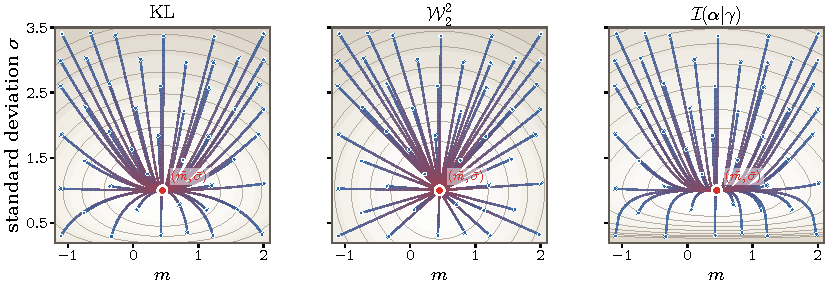
\includegraphics[width=.90\linewidth]{figures/gradflow-gaussian-1d-energy-landscapes/flows-focused.pdf}
\caption{\emph{One-dimensional Gaussian Wasserstein gradient flows in the Euclidean parameter half-plane $(m,\sigma)$.} From left to right, the panels show relative entropy, squared Wasserstein distance, and relative Fisher information. The same $48$ initial parameters are marked in blue; the trajectories progress through violet toward the common target $(\bar m,\bar\sigma)$ in red. Each background uses its own level scale to reveal the geometry of the corresponding energy. The $\Wass_2^2$ trajectories are straight rays, whereas the other functionals bend the evolution of the standard deviation.}
\label{fig:gradflow-gaussian-1d-energy-landscapes}
\end{figure}

\paragraph{Constrained evolution on the Gaussian manifold.}
\index{Gaussian!manifold}% strictindex

The preceding affine-gradient examples have a limited scope: most Wasserstein gradient flows of a functional \(f(\alpha)\) are not closed on the Gaussian manifold. A nonlinear ambient velocity creates higher-order moments immediately, so the exact Gaussian closure usually fails. The constrained viewpoint deliberately replaces the full evolution by its projection onto \(\mathcal G\), forcing the curve to remain Gaussian while keeping the Wasserstein tangent geometry.
\index{affine!closure}% strictindex
\index{Gaussian!projection}% strictindex

Let
\[
	\mathcal G=\{\Gaussian(m,\Sigma):m\in\RR^d,\ \Sigma\succ0\}
\]
be the Gaussian submanifold of $\Pp_2(\RR^d)$. The Wasserstein gradient of a functional constrained to a smooth submanifold $\mathcal M\subset\Pp_2$ is defined as the Riesz representative of the differential restricted to tangent velocities of $\mathcal M$. Formally, under local well-posedness and consistency assumptions, it is the small-step limit of the constrained JKO scheme
\index{Gaussian!submanifold}% strictindex
\index{Wasserstein!gradient}% strictindex
\index{JKO scheme}% strictindex
\[
	\alpha^{(\ell+1)}\in
	\uargmin{\alpha\in\mathcal M}
	\frac{1}{2\tau}\Wass_2^2(\alpha,\alpha^{(\ell)})+f(\alpha).
\]
For $\mathcal M=\mathcal G$, tangent velocities are affine gradient fields $v(x)=b+A(x-m)$ with $A=A^\top$. The constrained gradient is therefore the $L^2(\Gaussian(m,\Sigma))$ projection of the ambient Wasserstein gradient onto this finite-dimensional affine space, whenever the ambient gradient exists.
\index{affine!gradient}% strictindex
\index{Wasserstein!gradient}% strictindex

\begin{prop}[Gaussian-constrained Wasserstein gradients]\label{prop-gaussian-gradient-bullet-list}
	Let $f$ be a smooth functional and assume that its restriction to nondegenerate Gaussian measures can be written as
\index{Gaussian!measure}% strictindex
	\[
		f(\Gaussian(m,\Sigma))=F(m,\Sigma).
	\]
	Then the Wasserstein gradient constrained to the Gaussian family is the affine vector field
\index{Wasserstein!gradient}% strictindex
	\[
		v_F(x)
		=
		\nabla_m F(m,\Sigma)
		+
		2\nabla_\Sigma F(m,\Sigma)(x-m),
	\]
	where $\nabla_\Sigma F$ denotes the symmetric matrix derivative. Equivalently, $v_F$ is the $L^2(\Gaussian(m,\Sigma))$ projection of the ambient Wasserstein gradient onto affine gradient fields, whenever the ambient gradient exists. Hence the gradient descent flow constrained to Gaussian measures satisfies
\index{affine!gradient}% strictindex
\index{Wasserstein!gradient}% strictindex
\index{Gaussian!measure}% strictindex
	\begin{equation}\label{eq-gaussian-wgf-closure}
		\dot m_t=-\nabla_m F(m_t,\Sigma_t),
		\qquad
		\dot\Sigma_t=-2\bigl(\Sigma_t\nabla_\Sigma F(m_t,\Sigma_t)+\nabla_\Sigma F(m_t,\Sigma_t)\Sigma_t\bigr),
	\end{equation}
	and the descent velocity is affine.
\end{prop}

\begin{proof}
	Test the functional along a Gaussian tangent vector, represented by an affine gradient field
\index{affine!gradient}% strictindex
	\(v(x)=b+A(x-m)\)
	with $A$ symmetric. The induced first-order variations are $\dot m=b$ and $\dot\Sigma=A\Sigma+\Sigma A$. Therefore
	\[
		\d F(m,\Sigma)[b,A\Sigma+\Sigma A]
		=
		\dotp{\nabla_m F}{b}
		+
		\tr\!\left(\nabla_\Sigma F(A\Sigma+\Sigma A)\right).
	\]
	Since $A$, $\Sigma$ and $\nabla_\Sigma F$ are symmetric, the second term equals
	\[
		2\,\tr(\nabla_\Sigma F\,A\Sigma)
		=
		\int \dotp{2\nabla_\Sigma F(x-m)}{A(x-m)}\d\Gaussian(m,\Sigma)(x).
	\]
	Together with the mean term, this gives
	\[
		\d F(m,\Sigma)[\dot m,\dot\Sigma]
		=
		\int \dotp{v_F(x)}{v(x)}\d\Gaussian(m,\Sigma)(x)
	\]
	for all affine gradient fields $v$. This identifies the constrained Wasserstein gradient in the induced $L^2(\alpha)$ metric, or equivalently the projection of the ambient gradient when it exists. Substituting the descent velocity $-v_F$ in Proposition~\ref{prop-gaussian-affine-closure} gives~\eqref{eq-gaussian-wgf-closure}.
\index{Wasserstein!gradient}% strictindex
\index{affine!closure}% strictindex
\end{proof}

This proposition is the organizing rule for constrained Gaussian closures: once the scalar energy has been reduced to a function of $(m,\Sigma)$, its constrained Wasserstein gradient is automatically affine and the covariance follows the Bures-type ODE~\eqref{eq-gaussian-wgf-closure}. When the first variation of $f$ is quadratic, this constrained gradient coincides with the full Wasserstein gradient.
\index{first variation}% strictindex
\index{Gaussian!closure}% strictindex


\paragraph{Non-variational Gaussian-preserving flows.}
\index{Gaussian!preservation}% strictindex
\index{Gaussian!preserving flow}% strictindex

The following examples start from prescribed velocities rather than a fixed scalar energy. Their affine structure preserves Gaussianity. Special choices, such as the Ornstein--Uhlenbeck path, also admit a gradient-flow interpretation.
\index{velocity field}% strictindex
\index{Wasserstein!space}% strictindex
\index{Gaussian!measure}% strictindex
\index{gradient!flow}% strictindex

\begin{example}[Flow matching and diffusion paths between Gaussians]
	Consider a prescribed Gaussian interpolation $\alpha_t=\Gaussian(m_t,\Sigma_t)$. Proposition~\ref{prop-gaussian-affine-closure} supplies the unique minimum-energy continuity-equation velocity, with $A_t=A_t^\top$:
\index{affine!closure}% strictindex
\index{flow matching}% strictindex
	\[
		v_t(x)=\dot m_t+A_t(x-m_t),
		\qquad
		A_t\Sigma_t+\Sigma_t A_t=\dot\Sigma_t.
	\]
	This tangent field need not equal the regression field of a specified latent interpolant; Proposition~\ref{prop-gaussian-flow-matching-optimality} gives a counterexample when endpoint covariances do not commute. In the isotropic case $\Sigma_t=s_t^2\Id$, this reduces to the transparent formula $v_t(x)=\dot m_t+\frac{\dot s_t}{s_t}(x-m_t)$. For instance, the diffusion noising path $X_t=a_tX_0+\sigma_t Z$, where $Z\sim\Gaussian(0,\Id)$ is independent of $X_0$,
	has $m_t=a_tm_0$ and $\Sigma_t=a_t^2\Sigma_0+\sigma_t^2\Id$. Thus, in the Gaussian case, diffusion paths and flow-matching paths reduce to the same mean-covariance bookkeeping, although the corresponding training objectives are different.
\index{flow matching}% strictindex
\end{example}

\begin{example}[Gaussian kernel drifting]
\index{kernel!Gaussian}% strictindex
\index{Gaussian!kernel drifting}% strictindex
	Let the target be $\gamma=\Gaussian(\bar m,\bar\Sigma)$ and assume $\al_t=\Gaussian(m_t,\Sigma_t)$. For the Gaussian kernel
	\[
		K_\epsilon(x,y)=\exp(-\norm{x-y}^2/(2\epsilon)),
	\]
	the normalized field~\eqref{eq-normalized-kernel-drift} satisfies
	\[
		B_\epsilon[\al_t](x)
		=
		-\epsilon(\Sigma_t+\epsilon\Id)^{-1}(x-m_t).
	\]
	Indeed the smoothed density \(x\mapsto\int K_\epsilon(x,y)\d\al_t(y)\) is proportional to the Gaussian density with mean $m_t$ and covariance $\Sigma_t+\epsilon\Id$. Thus \(B_\epsilon[\al_t]\) is the mean-shift vector of a Gaussian density: it points linearly toward the Gaussian mode, with strength set by the bandwidth. The drifting velocity~\eqref{eq-cross-minus-self-drift} is therefore the difference of two affine mean-shift fields; it is affine and preserves Gaussianity. With $A_t=(\Sigma_t+\epsilon\Id)^{-1}$ and $\bar A=(\bar\Sigma+\epsilon\Id)^{-1}$, the ODE is
	\[
		\dot m_t=\epsilon\bar A(\bar m-m_t),
		\qquad
		\dot\Sigma_t=\epsilon\bigl((A_t-\bar A)\Sigma_t+\Sigma_t(A_t-\bar A)\bigr).
	\]
	This finite-dimensional model explains the stabilizing role of the self-normalized repulsion term in drifting: without it, the covariance equation loses the $A_t\Sigma_t+\Sigma_tA_t$ contribution.
\end{example}

\begin{example}[Gaussian closure of attention dynamics]
\index{Gaussian!closure}% strictindex
\index{attention}% strictindex
	For the transformer PDE~\eqref{eq-transformer-mean-field-pde}, assume $\alpha=\Gaussian(m,\Sigma)$. Exponential tilting gives directly
\index{transformer}% strictindex
	$\Gamma_\theta[\alpha](x)=Vm+V\Sigma K^\top Qx$, which is affine. While the following moment system has a finite solution with $\Sigma_t\succ0$, the Gaussian token law is preserved:
	\[
		\dot m_t=(V_t+V_t\Sigma_tK_t^\top Q_t)m_t,
		\qquad
		\dot\Sigma_t=B_t\Sigma_t+\Sigma_tB_t^\top,
		\qquad
		B_t=V_t\Sigma_tK_t^\top Q_t.
	\]
	When $V_t=Q_t^\top K_t$, the matrix $B_t=Q_t^\top K_t\Sigma_tK_t^\top Q_t$ is symmetric positive semidefinite, matching the gradient-field case mentioned above.
	This closure is not a convergence theorem for trained transformers. It is instead a tractable model of how attention can shear, amplify or contract a cloud of tokens through its covariance.
\index{transformer}% strictindex
\index{attention}% strictindex
\end{example}

\paragraph{Contractive Gaussian projection.}
\index{Gaussian!projection}% strictindex
\index{contractive Gaussian projection}% strictindex

The preceding examples show when Gaussianity is preserved or imposed by projection. Gelbrich's inequality~\citep{gelbrich1990formula} gives a useful variational explanation: replacing a measure by the Gaussian with the same first two moments cannot increase its Wasserstein distance to another similarly projected measure.
\index{Gelbrich inequality}% strictindex
\index{Wasserstein!distance}% strictindex

\begin{defn}[Gaussian projection]\label{def-gaussian-projection}
For \(\alpha\in\Pp_2(\RR^d)\), its Gaussian projection is
\[
	\GaussProj(\alpha)
	\eqdef
	\Gaussian(m_\alpha,\Sigma_\alpha),
\]
the Gaussian with the same mean and covariance as \(\alpha\).
\end{defn}

\begin{thm}[Gelbrich theorem]\label{thm-gelbrich-projection}
\index{Gelbrich theorem}% strictindex
	For every $\al,\be\in\Pp_2(\RR^d)$,
	\[
		\Wass_2^2\bigl(\GaussProj(\al),\GaussProj(\be)\bigr)
		=
		\norm{m_\al-m_\be}^2+\Bb^2(\Sigma_\al,\Sigma_\be)
		\leq
		\Wass_2^2(\al,\be).
	\]
\end{thm}

\begin{proof}
	Take any coupling $(X,Y)$ of $\al$ and $\be$, center the variables, and write $C=\EE[(X-m_\al)(Y-m_\be)^\top]$. In the positive definite case, positivity of the block covariance matrix implies the factorization $C=\Sigma_\al^{1/2}K\Sigma_\be^{1/2}$ with $\norm{K}_{\mathrm{op}}\leq1$, and therefore, by operator/nuclear norm duality, $\tr C\leq \tr\bigl((\Sigma_\al^{1/2}\Sigma_\be\Sigma_\al^{1/2})^{1/2}\bigr)$.
\index{covariance!matrix}% strictindex
	The semidefinite case follows by adding $\eta\Id$ to both covariance matrices and letting $\eta\downarrow0$.
	Expanding $\EE\norm{X-Y}^2$ gives the lower bound
	\[
		\EE\norm{X-Y}^2
		\geq
		\norm{m_\al-m_\be}^2+\Bb^2(\Sigma_\al,\Sigma_\be).
	\]
	Taking the infimum over couplings proves the inequality, while equality for Gaussian laws is Proposition~\ref{prop-gaussian-w2-bures}.
\end{proof}

For example, if $\gamma_i$ are Gaussian and $\lambda_i\geq0$, this contraction shows that projecting a competitor cannot increase $\sum_i\lambda_i\Wass_2^2(\alpha,\gamma_i)$. The same principle will now be applied to a full minimizing-movement step.

The following preservation criterion is a direct consequence of Gelbrich's theorem and was explained to us by Hugo Lavenant. It says that a functional which does not increase under moment-matched Gaussian projection admits Gaussian minimizing movements from Gaussian initial data.
\index{Gelbrich inequality}% strictindex
\index{moment matching}% strictindex
\index{Lavenant criterion}% strictindex
\index{Gaussian!projection}% strictindex
\index{minimizing movement}% strictindex
\index{Gelbrich theorem}% strictindex

\begin{thm}[Hugo Lavenant Gaussian-preservation criterion]\label{thm-lavenant-gaussian-preserving-jko}
\index{Gaussian!preservation}% strictindex
	Let $f:\Pp_2(\RR^d)\to(-\infty,+\infty]$ satisfy
	\[
		f\bigl(\GaussProj(\al)\bigr)\leq f(\al)
		\qquad\forall\al\in\Pp_2(\RR^d),
	\]
	with $\GaussProj$ defined in Definition~\ref{def-gaussian-projection}. If $\gamma$ is Gaussian and $\alpha^\star$ minimizes the JKO step
\index{Gelbrich inequality}% strictindex
	\[
		\eta\mapsto f(\eta)+\frac1{2\tau}\Wass_2^2(\gamma,\eta),
	\]
	then $\GaussProj(\alpha^\star)$ is also a minimizer. If this JKO minimizer is unique, it is Gaussian. Consequently, if every step from Gaussian data has a unique minimizer and the resulting minimizing movements converge in $\Wass_2$, each discrete iterate is Gaussian and every limit curve is Gaussian as well, possibly with a singular limiting covariance.
\index{Wasserstein!gradient}% strictindex
\index{gradient!flow}% strictindex
\index{Wasserstein!gradient flow}% strictindex
\index{JKO scheme}% strictindex
\end{thm}

\begin{proof}
	For the JKO claim, $\GaussProj(\gamma)=\gamma$ because $\gamma$ is Gaussian. Hence, for any competitor $\eta$,
	\[
		f\bigl(\GaussProj(\eta)\bigr)+\frac1{2\tau}\Wass_2^2\bigl(\gamma,\GaussProj(\eta)\bigr)
		\leq
		f(\eta)+\frac1{2\tau}\Wass_2^2(\gamma,\eta).
	\]
	Applying this to a minimizer $\eta=\alpha^\star$ shows that $\GaussProj(\alpha^\star)$ is again a minimizer. Uniqueness forces $\alpha^\star=\GaussProj(\alpha^\star)$. Iterating proves the discrete claim. Finally, Gaussian laws, allowing singular covariances, form a closed subset of $\Pp_2$: convergence in $\Wass_2$ gives convergence of their means and covariances, and hence of their Gaussian characteristic functions. This proves the limit claim.
\end{proof}

\paragraph{Moment closure beyond Gaussianity.}
\index{moment closure}% strictindex
\index{eikonal equation}% strictindex

Gaussian preservation concerns the full law, whereas moment closure asks only whether selected statistics obey an autonomous system. The first row of Proposition~\ref{prop-centered-gaussian-covariance-catalogue} in fact gives a distribution-free closure. If $f(\alpha)=g(m_\alpha,\Sigma_\alpha)$ and $G=\nabla_\Sigma g(m_\alpha,\Sigma_\alpha)$ denotes the symmetric Frobenius gradient, then the Wasserstein descent velocity is
\(v_\alpha(x)=-\nabla_m g(m_\alpha,\Sigma_\alpha)-2G(x-m_\alpha)\).
It is affine in $x$ for every $\alpha$, not only for Gaussian laws. Consequently, every sufficiently regular flow starting from $\alpha_0\in\Pp_2(\RR^d)$ satisfies the following system as long as its moments stay in the differentiability domain of $g$:
\begin{equation}\label{eq-distribution-free-mean-covariance-closure}
	\dot m_t=-\nabla_m g(m_t,\Sigma_t),
	\qquad
	\dot\Sigma_t
	=
	-2\bigl(\Sigma_t\nabla_\Sigma g(m_t,\Sigma_t)
	+\nabla_\Sigma g(m_t,\Sigma_t)\Sigma_t\bigr).
\end{equation}
For Gaussian initial data, this affine velocity also preserves Gaussianity; for general initial data, the law need not become Gaussian, but its mean and covariance still follow the same closed vector field $(h,H)$ listed in that proposition.

This suggests asking which linear statistics $\alpha\mapsto\int\varphi\,\d\alpha$ admit an exact closure. For scalar statistics, the answer is completely characterized by an eikonal equation.

\begin{prop}[Scalar moment closure and eikonal characterization]\label{prop-scalar-moment-closure}
	Let $\Omega\subset\RR^d$ be connected and open, let $\varphi\in C^2(\Omega)$, and set
	\(m_\varphi(\alpha)\eqdef\int_\Omega\varphi(x)\d\alpha(x)\)
	for $\alpha\in\Pp_2(\Omega)$ such that $\varphi$ and $\norm{\nabla\varphi}^2$ are integrable. We consider the unconstrained characteristic field while its trajectories remain in $\Omega$; boundary reflection or projection would change the calculation. For every smooth $g:\RR\to\RR$, the Wasserstein gradient flow of $f_g(\alpha)=g(m_\varphi(\alpha))$ satisfies, whenever the differentiation is justified,
	\[
		\dot m_t
		=
		-g'(m_t)\int_\Omega\norm{\nabla\varphi(x)}^2\d\alpha_t(x),
		\qquad m_t=m_\varphi(\alpha_t).
	\]
	This equation is autonomous for every $g$, meaning that its right-hand side depends on $\alpha_t$ only through $m_t$, if and only if there are constants $a,b\in\RR$ such that
	\begin{equation}\label{eq-scalar-moment-affine-carre}
		\norm{\nabla\varphi(x)}^2=a+b\varphi(x)
		\qquad (x\in\Omega).
	\end{equation}
	In that case, $\dot m_t=-(a+b m_t)g'(m_t)$.
	Moreover, on every connected open set $U\subset\{x:\nabla\varphi(x)\neq0\}$, the restriction of~\eqref{eq-scalar-moment-affine-carre} to $U$ is equivalent to the existence of an eikonal coordinate $r\in C^2(U)$ and constants $c,\kappa,\lambda\in\RR$ such that
	\begin{equation}\label{eq-scalar-moment-eikonal-form}
		\norm{\nabla r}=1,
		\qquad
		\varphi=c+\kappa r+\frac{\lambda}{2}r^2.
	\end{equation}
	For equivalence with the specified constants $a,b$ in~\eqref{eq-scalar-moment-affine-carre}, these parameters satisfy $2\lambda=b$ and $\kappa^2-2\lambda c=a$.
\end{prop}

\begin{proof}
	The first variation is $\delta f_g(\alpha)(x)=g'(m_\varphi(\alpha))\varphi(x)$, so the continuity equation gives the displayed evolution of $m_t$. Condition~\eqref{eq-scalar-moment-affine-carre} then proves sufficiency.

	For necessity, it is enough to take $g(s)=s$ and write $\psi=\norm{\nabla\varphi}^2$. Autonomy for Dirac laws first shows that $\psi=q\circ\varphi$ for some function $q$ on $\varphi(\Omega)$. Because $\Omega$ is connected, $\varphi(\Omega)$ is an interval. Comparing a Dirac law with any two-point mixture having the same $\varphi$-moment shows that
	\[
		q\bigl((1-\zeta)s_0+\zeta s_1\bigr)
		=
		(1-\zeta)q(s_0)+\zeta q(s_1)
		\qquad (0\leq\zeta\leq1).
	\]
	Hence $q$ is affine, which is precisely~\eqref{eq-scalar-moment-affine-carre}.

	On a regular set $U$, the right-hand side of~\eqref{eq-scalar-moment-affine-carre} is positive. Fix $s_0\in\varphi(U)$ and define $r(x)=\int_{s_0}^{\varphi(x)}(a+bs)^{-1/2}\d s$.
	Then $\norm{\nabla r}=1$. Inverting this change of variables gives~\eqref{eq-scalar-moment-eikonal-form} with $c=s_0$, $\kappa=\sqrt{a+bs_0}$, and $\lambda=b/2$. Conversely,~\eqref{eq-scalar-moment-eikonal-form} gives
	$\norm{\nabla\varphi}^2=\kappa^2-2\lambda c+2\lambda\varphi$.
\end{proof}

\begin{example}[A closed signed-distance moment]
	Let $\mathcal S$ be a $C^2$ hypersurface and let $r_{\mathcal S}$ be its signed distance on a sufficiently small tubular neighborhood $U$, where $\norm{\nabla r_{\mathcal S}}=1$. For
	$\varphi(x)=r_{\mathcal S}(x)+\lambda r_{\mathcal S}(x)^2/2$, one has $\norm{\nabla\varphi}^2=1+2\lambda\varphi$. Consequently, for any solution whose support remains in $U$, the scalar moment obeys $\dot m_t=-(1+2\lambda m_t)g'(m_t)$ under the objective $f_g(\alpha)=g(\int\varphi\,\d\alpha)$.
	For $\lambda=0$ and a genuinely curved $\mathcal S$, the observable is generally non-polynomial and the descent velocity is proportional to the non-affine normal field $\nabla r_{\mathcal S}$. This closure therefore does not arise from the mean--covariance mechanism above.
\end{example}


\section*{Conclusion}
\addcontentsline{toc}{section}{Conclusion}
The central message of this review is that many machine-learning methods can be read as PDEs on probability measures. Optimal transport supplies the geometry behind this statement: it turns a loss into a metric gradient flow, a coupling into a geodesic, a score into a Fokker--Planck drift, and a generative model into a transported law. This language is valuable because it separates modelling choices from representation choices. A finite particle algorithm, a neural parametrization and a continuum PDE may then be understood as different approximations of the same measure-valued evolution.

The same viewpoint also clarifies the limits of current theory. Empirical measures are singular, neural parametrizations are non-convex, high-dimensional transport is statistically expensive, and generative flows often use interpolants that are transportation dynamics without being Wasserstein geodesics or gradient flows. These tensions are not defects of the PDE viewpoint; they identify where mathematical analysis is still needed. For machine learning, PDEs are therefore both an explanatory tool and a source of new problems.

\section*{Competing interests}
The author declares no competing interests.

\section*{Data availability statement}
No new data were generated for this review. The manuscript sources and the code used to generate the numerical figures are available at \url{https://github.com/gpeyre/ot4ml}.

\begingroup
\sloppy
\hfuzz=1pt
\setlength{\emergencystretch}{2em}
\bibliographystyle{plainnat}
\bibliography{all}
\endgroup

\end{document}
